\PassOptionsToPackage{dvipsnames,svgnames,table}{xcolor}
\documentclass[10pt]{article}
\usepackage[a4paper,margin=22mm]{geometry}
\usepackage[no-math]{fontspec}
\setmainfont{Latin Modern Roman}
\usepackage{amsmath,amssymb,amsthm,amscd,latexsym,tikz,graphicx,xcolor,cite,hyperref,xurl}
\setlength{\emergencystretch}{4em}
\SetMathAlphabet{\mathbf}{normal}{OT1}{cmr}{bx}{n}
\SetMathAlphabet{\mathbf}{bold}{OT1}{cmr}{bx}{n}
\newtheorem{theorem}{Theorem}[section]
\newtheorem{lemma}[theorem]{Lemma}
\newtheorem{prop}[theorem]{Proposition}
\newtheorem{coro}[theorem]{Corollary}
\theoremstyle{definition}
\newtheorem{defi}[theorem]{Definition}
\newtheorem{exam}[theorem]{Example}
\newtheorem{rema}[theorem]{Remark}
\numberwithin{equation}{section}
\newtheorem{introtheorem}{Theorem}
\renewcommand*{\theintrotheorem}{\Alph{introtheorem}}
% Scaffold existence declarations solely for two unused native renewcommands.
\newcommand{\UParrow}{\PackageError{alco260}{Unused arrow helper expanded outside retained scope}{}}
\newcommand{\DOWNarrow}{\PackageError{alco260}{Unused arrow helper expanded outside retained scope}{}}
% Unavailable script-font helpers are inactive and preserved, with strict expansion rejection.
\newcommand{\mathscr}[1]{\PackageError{alco260}{Uninventoried script helper expanded}{}}
\newfontfamily\CorpusUpDots[Path=/usr/share/texmf/fonts/opentype/public/lm-math/]{latinmodern-math.otf}
\newcommand{\iddots}{\mathinner{\text{\CorpusUpDots\char"22F0}}}
\renewcommand{\theenumi}{\roman{enumi}}
\renewcommand{\labelenumi}{(\theenumi)}

\let\<\langle
\let\>\rangle

\newcommand\Comment[2][\relax]{\space\par\medskip\noindent
   \fbox{\begin{minipage}{\textwidth}\textbf{Comment\ifx\relax#1\else---#1\fi}\newline
        #2\end{minipage}}\medskip
}

\def\ocirc#1{\stackrel{_{\,\circ}}{#1}}


\DeclareMathOperator\ldom {\triangleleft}
\DeclareMathOperator\ledom{\trianglelefteq}
\DeclareMathOperator\gdom {\triangleright}
\DeclareMathOperator\gedom{\trianglerighteq}

\def\bi{\text{\boldmath$i$}}
\def\bgg{\text{\boldmath$g$}}
\def\bj{\text{\boldmath$j$}}
\def\bm{\text{\boldmath$m$}}
\def\bk{\text{\boldmath$k$}}
\def\bl{\text{\boldmath$l$}}
\def\bs{\text{\boldmath$s$}}
\def\bt{\text{\boldmath$t$}}
\def\bc{\text{\boldmath$c$}}
\def\br{\text{\boldmath$r$}}
\def\b1{\text{\boldmath$1$}}

\def\bI{\text{\boldmath$I$}}
\def\ba{\text{\boldmath$a$}}
\def\bb{\text{\boldmath$b$}}
\def\bla{\text{\boldmath$\lambda$}}

\def\pmod#1{\text{ }(\text{\rm mod } #1)\,}

\def\bijection{\overset{\sim}{\longrightarrow}}

\newcommand\Haff[1][d]{H^\infty_{#1}}

\newcommand{\Hom}{\operatorname{Hom}}
\newcommand{\Ext}{\operatorname{Ext}}
\newcommand{\EXT}{\operatorname{Ext}}
\newcommand{\ext}{\operatorname{ext}}

\newcommand{\End}{\operatorname{End}}
\newcommand{\ind}{\operatorname{ind}}
\newcommand{\im}{\operatorname{im}}
\newcommand{\id}{\operatorname{id}}

\def\sgn{\mathtt{sgn}}
\newcommand{\res}{\operatorname{res}}
\newcommand{\height}{\operatorname{ht}}
\newcommand{\soc}{\operatorname{soc}\,}
\newcommand{\head}{\operatorname{head}}
\newcommand{\og}{\operatorname{res}}
\newcommand{\mo}{\operatorname{mod}}
\newcommand{\modu}{\operatorname{mod-}}
\newcommand{\cha}{\operatorname{char}}
\newcommand{\St}{\operatorname{St}}
\newcommand{\infl}{\operatorname{dil}}
\newcommand{\shr}{\operatorname{shr}}
\newcommand{\trun}{\operatorname{trun}}
\newcommand{\AFF}{\operatorname{A\Gamma L}}
\newcommand{\PRO}{\operatorname{P\Gamma L}}
\newcommand{\PROU}{\operatorname{P\Gamma U}}
\newcommand{\Stab}{\operatorname{Stab}}
\newcommand{\lcm}{\operatorname{lcm}}

\newcommand{\Z}{\mathbb{Z}}

\newcommand{\N}{\mathcal{N}}
\newcommand{\SSSS}{\mathcal{S}}
\newcommand{\SSSSS}{\boldsymbol{\mathcal{S}}}
\newcommand{\0}{{\bar 0}}

\def\eps{{\varepsilon}}
\def\phi{{\varphi}}

\newcommand{\catA}{{\mathbf A}}
\newcommand{\catB}{{\mathbf B}}
\newcommand{\catC}{{\mathbf C}}
\newcommand{\catD}{{\mathbf D}}

\newcommand{\bq}{\mathbf{q}}

\newcommand\gldim{\operatorname{gl.dim\,}}
\newcommand\pd{\operatorname{proj.dim\,}}

\newcommand{\funF}{{\mathcal F}}
\newcommand{\funQ}{{\mathcal Q}}
\newcommand{\funP}{{\mathcal P}}
\newcommand{\funR}{{\mathcal R}}
\newcommand{\funE}{{\mathcal E}}
\newcommand{\funO}{{\mathcal O}}
\newcommand{\Fil}{{\tt Fil}}

\newcommand{\ga}{\gamma}
\newcommand{\Ga}{\Gamma}
\newcommand{\la}{\lambda}
\newcommand{\La}{\Lambda}
\newcommand{\al}{\alpha}
\newcommand{\be}{\beta}
\newcommand{\ep}{\epsilon}
\newcommand{\Si}{\Sigma}
\newcommand{\si}{\sigma}
\newcommand{\ttt}{{\tt t}}
\newcommand{\om}{\omega}
\newcommand{\Om}{\Omega}
\newcommand{\vare}{\varepsilon}
\newcommand{\fee}{\varphi}
\newcommand{\de}{\delta}
\newcommand{\De}{\Delta}
\newcommand{\ka}{\kappa}
\def\triv#1{\O_{#1}}
\def\sign#1{\O_{-#1}}
\def\Belt{\mathbf{B}}


\newcommand{\NEarrow}{\mathbin{\rotatebox[origin=c]{45}{$\Rightarrow$}}}
\newcommand{\SEarrow}{\mathbin{\rotatebox[origin=c]{-45}{$\Rightarrow$}}}
\renewcommand{\UParrow}{\mathbin{\rotatebox[origin=c]{90}{$\Rightarrow$}}}
\renewcommand{\DOWNarrow}{\mathbin{\rotatebox[origin=c]{-90}{$\Rightarrow$}}}


\newcommand{\Ze}{{\mathbb Z}}
\newcommand{\Mull}{{\bf M}}

\def\Mtype{\mathtt{M}}
\def\Qtype{\mathtt{Q}}

\renewcommand\H[1][\Lambda]{\mathscr H^{#1}}
\newcommand\Hdel[1][k]{\mathscr H^\infty_{#1\delta}}

\newcommand{\Ker}{\operatorname{Ker}}
\newcommand{\Aut}{{\mathrm {Aut}}}
\newcommand{\Out}{{\mathrm {Out}}}
\newcommand{\Mult}{{\mathrm {Mult}}}
\newcommand{\Inn}{{\mathrm {Inn}}}
\newcommand{\Irr}{{\mathrm {Irr}}}
\newcommand{\IBR}{{\mathrm {IBr}}}

\newcommand{\ord}{{\mathrm {ord}}}
\def\id{\mathop{\mathrm {id}}\nolimits}
\renewcommand{\Im}{{\mathrm {Im}}}
\newcommand{\Ind}{{\mathrm {Ind}}}
\newcommand{\Coind}{{\mathrm {Coind}}}
\newcommand{\diag}{{\mathrm {diag}}}
\newcommand{\dist}{{\mathrm {dist}}}

\newcommand{\sol}{{\mathrm {sol}}}

\newcommand{\Mor}{{\mathrm {Mor}}}
\newcommand{\Mat}{{\mathrm {Mat}}}
\def\rank{\mathop{\mathrm{ rank}}\nolimits}
\newcommand{\Syl}{{\mathrm {Syl}}}
\newcommand{\Tr}{{\mathrm {Tr}}}
\newcommand{\tr}{{\mathrm {tr}}}
\newcommand{\Gal}{{\it Gal}}
\newcommand{\Spec}{{\mathrm {Spec}}}
\newcommand{\ad}{{\mathrm {ad}}}
\newcommand{\Sym}{{\mathrm {Sym}}}
\newcommand{\Char}{{\mathrm {char}}}
\newcommand{\pr}{{\mathrm {pr}}}
\newcommand{\rad}{{\mathrm {rad}\,}}
\newcommand{\abel}{{\mathrm {abel}}}
\newcommand{\codim}{{\mathrm {codim}}}

\newcommand{\Res}{{\mathrm {Res}}}
\newcommand{\Ann}{{\mathrm {Ann}}}

\newcommand{\Cbb}{{\mathbb C}}
\newcommand{\Q}{{\mathbb Q}}
\newcommand{\CL}{{\mathcal C}}
\newcommand{\SCL}{{\mathcal S}}
\newcommand{\RR}{{\mathbb R}}
\newcommand{\QQ}{{\mathbb Q}}
\newcommand{\ZZ}{{\mathbb Z}}
\newcommand{\NN}{{\mathbb N}}
\newcommand{\EE}{{\mathbb E}}
\newcommand{\PP}{{\mathbb P}}
\newcommand{\A}{{\mathscr A}}
\newcommand{\D}{{\mathcal D}}
\newcommand{\NC}{{\mathcal N}}
\newcommand{\MC}{{\mathcal M}}
\newcommand{\UC}{{\mathcal U}}
\newcommand{\IC}{{\mathcal I}}
\newcommand\Idel[1][k]{\IC_{#1\delta}}
\newcommand{\BC}{{\mathcal B}}
\newcommand{\GC}{{\mathcal G}}
\newcommand{\EC}{{\mathcal E}}
\newcommand{\GD}{G^{*}}
\newcommand{\FF}{{\mathbb F}}
\newcommand{\FQ}{\FF_{q}}
\newcommand{\SSS}{{\sf S}}
\newcommand{\AAA}{{\sf A}}
\newcommand{\NNN}{{\mathcal N}}
\newcommand{\so}{{\sf S}}
\newcommand{\no}{{\sf N}}
\newcommand{\ea}{{\sf E}}
\newcommand{\we}{{\sf W}}
\newcommand{\T}{{\sf T}}
\newcommand{\nnee}{{\sf NE}}
\newcommand{\nnww}{{\sf NW}}
\newcommand{\ssee}{{\sf SE}}
\newcommand{\ssww}{{\sf SW}}
\newcommand{\SC}{{S_{\CC}}}
\newcommand{\LC}{{L_{\CC}}}
\newcommand{\SF}{{S_{\FF}}}
\newcommand{\VC}{{V_{\CC}}}
\newcommand{\WN}{{W_{\CC}}}
\newcommand{\dvg}{{d_{V}(g)}}
\newcommand{\dar}{{\downarrow}}
\newcommand{\uar}{{\uparrow}}
\newcommand{\ml}{{\mathfrak{m}_{\ell}}}
\newcommand{\mc}{{\mathfrak{m}_{\CC}}}
\newcommand{\dl}{{\mathfrak{d}_{\ell}}}
\newcommand{\tri}{\,{\trianglerighteq}\,}
\newcommand{\tn}{\hspace{0.5mm}^{t}\hspace*{-0.2mm}}
\newcommand{\ta}{\hspace{0.5mm}^{2}\hspace*{-0.2mm}}
\newcommand{\tb}{\hspace{0.5mm}^{3}\hspace*{-0.2mm}}
\def\skipa{ \vspace{-1.1mm} & \vspace{-1.1mm} & \vspace{-1.1mm}\\}
\def\skipb{\vspace{-1.3mm} & \vspace{-1.3mm} & \vspace{-1.3mm}\\}
\renewcommand{\mod}{\bmod \,}
\newcommand{\JS}{\operatorname{JS}}
\newcommand{\Sh}{\operatorname{Sh}}
\newcommand{\hc}{\operatorname{hc}}

\newcommand{\tw}{{\tt s}}

\newcommand{\blam}{\boldsymbol{\lambda}}
\newcommand{\bkap}{\boldsymbol{\kappa}}
\newcommand{\btau}{\boldsymbol{\tau}}
\newcommand{\bbep}{\boldsymbol{\varepsilon}}
\newcommand{\bmu}{\boldsymbol{\mu}}
\newcommand{\bnu}{\boldsymbol{\nu}}
\newcommand{\bbeta}{\boldsymbol{\beta}}
\newcommand{\brho}{\boldsymbol{\rho}}
\newcommand{\bxi}{\boldsymbol{\xi}}
\newcommand{\bzeta}{\boldsymbol{\zeta}}
\newcommand{\eeta}{\boldsymbol{\eta}}
\newcommand{\cB}{\mathcal{B}}




\newcommand{\sfr}{{\mathfrak{s}}}
\newcommand{\tfr}{{\mathfrak{t}}}
\newcommand{\sfrs}{{\mathfrak{s}}^{\star}}
\newcommand{\OLA}{{O_{\ell'}}}
\newcommand{\OLB}{{O_{\ell}}}
\newcommand{\FQT}{\FF_{q}^{\times}}
\newcommand{\IBr}{{\mathrm {IBr}}}
\def\h{{\mathfrak h}}
\def\g{{\mathfrak g}}
\def\n{{\mathfrak n}}
\def\aff{{\operatorname{aff}}}
\def\fin{{\operatorname{fin}}}
\def\rev{{\operatorname{rev}}}
\def\cont{{\operatorname{cont}}}
\def\init{{\operatorname{init}}}
\def\height{{\operatorname{ht}}}
\def\seq{{\operatorname{seq}}}


\def\Par{{\mathscr P}}
\def\ula{{\underline{\lambda}}}
\def\umu{{\underline{\mu}}}
\def\unu{{\underline{\nu}}}
\def\uka{{\underline{\kappa}}}

\def\f{{\mathbf{f}}}
\def\b{\mathfrak{b}}
\def\k{\Bbbk}
\def\x{x}
\def\W{\langle I \rangle}
\def\y{y}


\def\Comp{{\mathscr C}^l}
\def\cH{\H^\cl}
\def\fH{\H^\fn}
\def\U{{\mathtt U}}
\def\Stab{{\mathtt S}}
\def\G{{\mathtt G}}
\def\sh{{\operatorname{sh}}}
\def\nslash{\:\notslash\:}
\def\defect{\operatorname{def}}
\def\codeg{\operatorname{codeg}}
\def\spa{\operatorname{span}}
\def\height{{\operatorname{ht}}}
\def\lex{<_{\operatorname{lex}}}
\def\wt{{\operatorname{wt}}}
\def\RPart{{\mathscr{RP}}^{\La^t}}
\def\RPar{{\mathscr{RP}}^\kappa}
\def\surj{{\twoheadrightarrow}}
\def\Gar{{\operatorname{Gar}}}
\def\op{{\mathrm{op}}}
\def\re{{\mathrm{re}}}
\def\im{{\mathrm{im}\,}}
\def\onto{{\twoheadrightarrow}}
\def\into{{\hookrightarrow}}
\def\Mod#1{#1\!\operatorname{-Mod}}
\def\mod#1{#1\!\operatorname{-mod}}
\def\Proj#1{\text{{$\operatorname{Proj}$}(}#1{)}}

\def\gmod#1{#1\!\operatorname{-gmod}}
\renewcommand\O{\mathcal O}
\def\HCI{I}
\def\HCR{{}^*I}
\def\iso{\stackrel{\sim}{\longrightarrow}}
\def\B{{\mathcal B}}
\def\Pol{{\mathscr P}}
\def\Mde{M}
\def\Sde{S}
\def\Zde{Z}
\def\Lade{\La}
\def\Yde{Y}
\def\Sdot{S}
\def\Ladot{\La}
\def\Zdot{Z}
\def\Lde{L}
\def\Dede{\De}
\def\nade{\nabla}
\def\Tde{T}
\def\Pde{P}
\def\triv{{\tt triv}}
\def\ch{\operatorname{ch}}
\def\lan{\langle}
\def\ran{\rangle}
\def\HOM{\operatorname{Hom}}
\def\END{\operatorname{End}}
\def\Stand{\bar\Delta}
\def\Perm{\operatorname{Per}}
\def\SPerm{\operatorname{SPer}}
\def\CH{{\operatorname{ch}_q\,}}
\def\DIM{{\operatorname{dim}_q\,}}
\def\RANK{{\operatorname{rank}_q\,}}
\def\co{{\operatorname{col}}}
\def\words{I}
\def\shift{{\tt sh}}
\def\mul{{\tt mul}}
\def\Seq{{\tt Se}}
\def\Car{{\tt C}}
\def\cc{{\tt c}}
\def\Alc{{\mathcal C}}
\def\barinv{\mathtt{b}}
\newcommand{\bC}{\mathbf{C}}

\newcommand{\Zig}{\textsf{Z}}
\newcommand{\ze}{\textsf{e}}
\newcommand{\zm}{\textsf{m}}
\newcommand{\za}{\textsf{a}}
\newcommand{\zc}{\textsf{c}}
\newcommand{\CZig}{\textsf{C}}

\newcommand\SetBox[2][35mm]{\Big\{\vcenter{\hsize#1\centering#2}\Big\}}


{\catcode`\|=\active
  \gdef\set#1{\mathinner{\lbrace\,{\mathcode`\|"8000
  \let|\midvert #1}\,\rbrace}}
}
\def\midvert{\egroup\mid\bgroup}


\colorlet{darkgreen}{green!50!black}
\tikzset{dots/.style={very thick,loosely dotted},
         greendot/.style={fill,circle,color=darkgreen,inner sep=1.5pt,outer sep=0}
}
\def\greendot(#1,#2){\node[greendot] at(#1,#2){}}

\newenvironment{braid}{
  \begin{tikzpicture}[baseline=6mm,blue,line width=1pt, scale=0.4,
                      draw/.append style={rounded corners},
                      every node/.append style={font=\fontsize{5}{5}\selectfont}]
  }{\end{tikzpicture}
}
\newcommand\iicrossing[1][i]{ 
  \begin{braid}\tikzset{baseline=0mm,scale=0.5}
    \useasboundingbox (-0.6,0) rectangle (1,1.9);
    \draw(0,1)node[left=-1mm]{$#1$}--(1,0);
    \draw(1,1)node[right=-1mm]{$#1$}--(0,0);
  \end{braid}
}
\newcommand\iisquare[1][i]{
  \begin{braid}\tikzset{baseline=0mm,scale=0.7}
    \useasboundingbox (-0.6,0) rectangle (1,1.9);
    \draw(0,1)node[left=-1mm]{$#1$}--(1,0.5)--(0,0);
    \draw(1,1)node[right=-1mm]{$#1$}--(0,0.5)--(1,0);
  \end{braid}
}
\def\Grid(#1,#2){
  \draw[very thin,gray,step=2mm] (0,0)grid(#1,#2);
  \draw[very thin,darkgreen,step=10mm] (0,0)grid(#1,#2);
}

\newcommand\Tableau[2][\relax]{
  \begin{tikzpicture}[scale=0.5,draw/.append style={thick,black}]
    \ifx\relax#1\relax
    \else 
      \foreach\box in {#1} { \filldraw[blue!30]\box+(-.5,-.5)rectangle++(.5,.5); }
    \fi
    \newcount\row\newcount\col
    \row=0
    \foreach \Row in {#2} {
       \col=1
       \foreach\k in \Row {
          \draw(\the\col,\the\row)+(-.5,-.5)rectangle++(.5,.5);
          \draw(\the\col,\the\row)node{\k};
          \global\advance\col by 1
       }
       \global\advance\row by -1
    }
  \end{tikzpicture}
}

\newcommand{\hackcenter}[1]{\vcenter{\hbox{#1}}}


\newcommand\YoungDiagram[2][\relax]{
  \begin{tikzpicture}[scale=0.5,draw/.append style={thick,black}]
    \ifx\relax#1\relax
    \else 
    \foreach\box in {#1} {
      \filldraw[blue!30]\box rectangle ++(1,1);
    }
    \fi
    \newcount\row
    \row=0
    \foreach \col in {#2} {
       \draw(1,\the\row)grid ++(\col,1);
       \global\advance\row by -1
    }
  \end{tikzpicture}
}


\colorlet{darkgreen}{green!50!black}
\tikzset{dots/.style={very thick,loosely dotted},
         greendot/.style={fill,circle,color=darkgreen,inner sep=1.5pt,outer sep=0},
         blackdot/.style={fill,circle,color=black,inner sep=2pt,outer sep=0},
         graydot/.style={fill,circle,color=gray,inner sep=1.1pt,outer sep=0}
}
\def\greendot(#1,#2){\node[greendot] at(#1,#2){}}
\def\blackdot(#1,#2){\node[blackdot] at(#1,#2){}}
\def\graydot(#1,#2){\node[graydot] at(#1,#2){}}
\begin{document}
\section*{1105. Complete irredundant classification of cuspidal skew shapes in affine type A}
Dina Abbasian, Lena Difulvio, Robert Muth, Gabrielle Pasternak, Isabella Sholtes and Frances Sinclair. \emph{Cuspidal ribbon tableaux in affine type A}, Algebraic Combinatorics 6(2) (2023), 285--319. \url{https://doi.org/10.5802/alco.260}. Original publisher version; CC BY 4.0, \url{https://creativecommons.org/licenses/by/4.0/}.\par
\paragraph{Selected problem.} Prove the author's Theorem 6.13, located below with its complete terminal proof and preceding local core.
\paragraph{Source-context disclosure (editorial).} Original native line 2290 uses the literal \(\nu_1,\nu_t,\nu_h\) chain despite the preceding \(w^i\) path and removable-prefix argument. Lines 2281--2303 are retained unchanged, including that preceding argument; no replacement chain is supplied. Native line 2307 says \(t\in\mathcal N_t\), beside the preceding distinguished choices and Proposition 5.9 using \(t\in\mathbb Z_e\). Case 5 at line 2513 names \(\xi^\tau_{SE(z),w}\), while lines 2497 and 2508--2509 name the two shifted endpoints and their content equality. Lines 2430--2523 retain all six cases. In supporting Lemma 6.9, line 2751 binds uppercase \(\Lambda\) beside lowercase \(\lambda\) summands; lines 2744--2757 preserve the exact tile definitions and argument. In supporting Lemma 6.11, line 2775 writes \([1,\Lambda]\) beside the preceding \([1,|\Lambda|]\) index ranges; its complete proof remains literal. These are bounded source disclosures, not editorial formula corrections or independently supplied proofs.
\paragraph{Typography and scope (editorial).} All 45 inventoried arguments of the author's \texttt{hackcenter} are unchanged native TikZ. The wrapper uses standard \texttt{vcenter/hbox} for placement, replacing only the author's unavailable XY centering box; baseline and box-class placement may differ. Exactly two script-style upward diagonal ellipses use installed Latin Modern Math U+22F0 as a mathematical inner atom; stroke, width, scale and placement may differ from the original three-dot construction. No generic XY or mathdots implementation is supplied. Original unused package imports/declarations remain in archived native evidence. References to later unselected Sections 7--8 are rendered as their original printed numbers; the full original article remains the reference for that later program. Every retained primary statement, full proof and local new-core proof is editable native TeX.
\clearpage
% BEGIN EXACT-ORDER AUTHOR BODY, NATIVE 546--2828
\section{Introduction}

We begin by briefly describing the combinatorial data studied herein, referring the reader to the body of the paper for detailed exposition and to Example~\ref{BigEx} for demonstrative visuals.

Fix \(e > 1\), and let \(\Phi_+ = \Phi_+^\re \sqcup \Phi_+^\im\) be the positive root system of type \({\tt A}^{(1)}_{e-1}\); \(I = \{\alpha_0, \ldots, \alpha_{e-1}\}\) be the set of simple roots; \(Q_+ = \ZZ_{\geq 0}I\) be the root lattice;  \(\Phi_+^\re\) be the set of real roots; \(\Phi_+^\im = \{m \delta \mid m \in \NN\}\) be the set of imaginary roots, and \(\delta = \alpha_0 + \cdots + \alpha_{e-1}\) be the null root. We fix a convex preorder \(\succeq\) on \(\Phi_+\), see \S\ref{posrootsec}. This root system data is fundamental in the representation theory of the Kac-Moody Lie algebra \(\widehat{\mathfrak{sl}}_e\) \cite{KacBookInfLie}, and convex preorders determine PBW bases for the associated quantum group \cite{BeckConBas}.


A skew shape \(\tau\) is a set difference of Young diagrams. Nodes in \(\tau\) have residue in \(\ZZ_e\), and the skew shape \(\tau\) has content \(\cont(\tau) \in Q_+\), see \S\ref{skewshapesec}, \S\ref{contentsec}.
We say a set \(\Lambda\) of non-overlapping skew shapes is a tiling of a skew shape \(\tau\) provided that \(\tau = \bigsqcup_{\lambda \in \Lambda}\lambda\), and we refer to elements of \(\Lambda\) as tiles. A \(\Lambda\)-tableau \(\ttt = (\lambda_1, \ldots, \lambda_{|\Lambda|})\)  is an ordering of the tiles in \(\Lambda\) such that no node in \(\lambda_i\) is (weakly) southeast of any node in \(\lambda_j\) when \(1 \leq i < j \leq |\Lambda|\), see \S\ref{tilingsec}. This is a generalization of the notion of {\em Young} tableaux, in which each \(\lambda_i\) consists of a single node. Young tableaux and their associated residue sequences correspond to bases and associated weight spaces for Specht modules over cyclotomic Hecke algebras, and the symmetric group in particular, see \cite{MathasBookHecke, KlBookLinProj}.

Of particular interest in this paper are tilings whose constituent tiles are ribbons---connected skew shapes that contain no \(2 \times 2\) boxes.
Ribbon tilings and tableaux are well-studied combinatorial objects connected to many areas of algebra and geometry, such as the theory of symmetric functions, the representation theory of finite groups, Lie algebras and quantum groups, and the geometry of flag varieties, see \cite{FoStRimHk, LLTRibbon, ShefRib} for a few examples. The majority of research done on this topic concerns \(r\)-ribbon tableaux, in which all tiles are ribbons of a given cardinality \(r\). We do not include that restriction here, as we are interested in {\em cuspidal} ribbons, which have varying and unbounded cardinality.


\subsection{Cuspidality}\label{cuspint}
Motivated by the representation theory of Khovanov-Lauda-Rouquier (KLR) algebras studied in \cite{KlCuspSys, KlMuStrat, McNRepKLR3}, we introduce the notion of {\em cuspidal} and {\em semicuspidal} skew shapes. Let \(\tau\) be a skew shape such that \(\cont(\tau) = m \beta\) for some \(m \in \NN\) and \(\beta \in \Phi_+\). We say that \(\tau\) is semicuspidal provided that whenever \((\lambda_1, \lambda_2)\) is a tableau for \(\tau\), we may write \(\cont(\lambda_1)\) as a sum of positive roots \(\preceq \beta\), and \(\cont(\lambda_2)\) as a sum of positive roots \(\succeq \beta\). We say that \(\tau\) is cuspidal provided that \(m=1\) and the comparisons above may be made strict, see Definition~\ref{cuspdef}. 
We give a complete classification of cuspidal and semicuspidal skew shapes in Theorems~\ref{allcusp} and~\textup{7.18}, summarized (in a slightly weaker form) as Theorems~\ref{THMA} and~\ref{THMB} below.

\begin{introtheorem}\label{THMA}
Every cuspidal skew shape is a ribbon.
There exists a unique cuspidal ribbon \(\zeta^\beta\) of content \(\beta\) for all \(\beta \in \Phi_+^\re\), and \(e\) distinct cuspidal ribbons \(\zeta^{\overline{0}}, \ldots, \zeta^{\overline{e-1}}\) of content \(\delta\). 
\end{introtheorem}

\begin{introtheorem}\label{THMB}
Let \(m \in \NN\).
There exists a unique semicuspidal skew shape \(\zeta^{m \beta}\) of content \(m \beta\), for all \(\beta \in \Phi_+^\re\). The set of connected semicuspidal skew shapes of content \(m \delta\) is in bijection with \(\ZZ_e \times \SSSS_{\tt c}(m)\), where \(\SSSS_{\tt c}(m)\) is the set of connected skew shapes of cardinality \(m\). 
\end{introtheorem}

The uniqueness statements in Theorems~\ref{THMA} and~\ref{THMB} refer to uniqueness up to certain residue-preserving translations, see \S\ref{similaritysec}. In \S\ref{cuspcons} and \S\textup{7} we provide explicit constructions of all cuspidal and semicuspidal skew shapes. Imaginary semicuspidal skew shapes are constructed via an \(e\)-dilation process which is in some sense an inversion of the \(e\)-quotients defined in \cite{LittlewoodModRep}.

\subsection{Kostant tilings}\label{Kosint}
Let \(\Lambda\) be a tiling for \(\tau\). We say a \(\Lambda\)-tableau \(\ttt = (\lambda_1, \ldots, \lambda_{|\Lambda|})\) is {\em Kostant} if there exist \(m_1, \ldots, m_k \in \NN\), \(\beta_1\succeq \ldots \succeq \beta_k \in \Phi_+\) such that \(\cont(\lambda_i) = m_i \beta_i\) for all \(1 \leq i \leq |\Lambda|\). We say it is {\em strict} Kostant if the comparisons above are strict. We say \(\Lambda\) is a {\em (strict) Kostant} tiling if a (strict) Kostant \(\Lambda\)-tableau exists. We say that a tiling is {\em cuspidal} (resp. {\em semicuspidal}) if every constituent tile is a cuspidal (resp. {\em semicuspidal}) skew shape. 

If \(\cont(\tau) = \theta\), then a Kostant tiling \(\Lambda\) of \(\tau\) may naturally be associated with a Kostant partition \(\bkap^\Lambda\) of \(\theta\), see \S\ref{Kostsec}. The convex preorder \(\succeq\) naturally induces a bilexicographic partial order \(\trianglerighteq\) on the set \(\Xi(\theta)\) of Kostant partitions of \(\theta\). Our main theorem on Kostant tilings is the following, which appears as Theorems~\ref{mainthmcusp} and~\textup{7.19} in the text:

\begin{introtheorem}\label{THMC}
Let \(\tau\) be a nonempty skew shape.
\begin{enumerate}
\item There exists a unique cuspidal Kostant tiling \(\Gamma_\tau\) for \(\tau\). \label{cond:C1}
\item There exists a unique semicuspidal strict Kostant tiling \(\Gamma^{sc}_\tau\) for \(\tau\). \label{cond:C2}
\item If \(\Lambda\) is any Kostant tiling for \(\tau\), then we have \( \bkap^{\Lambda} \trianglelefteq \bkap^{\Gamma_\tau} = \bkap^{\Gamma^{sc}_\tau} \). \label{cond:C3}
\end{enumerate}
\end{introtheorem}

We establish existence in Theorem~\ref{THMC}\eqref{cond:C1},\eqref{cond:C2} constructively;
in \S\ref{resKos} we show the cuspidal Kostant tiling \(\Gamma_\tau\) may be constructed via progressive removal of {\em minimal ribbons}.

\subsection{Application to representation theory} 

The combinatorial study of cuspidality and Kostant tilings for skew shapes discussed in \S\ref{cuspint}, \S\ref{Kosint} is motivated by a connection to the theory of cuspidal systems and Specht modules over Khovanov-Lauda-Rouquier (KLR) algebras, and has application in that setting.

For any field \(\k\) and \(\theta \in Q_+\), there is an associated KLR \(\k\)-algebra \(R_\theta\). This family of algebras categorifies the positive part of the quantum group \(U_q(\widehat{\mathfrak{sl}}_e)\), see \cite{KhoLauDiagCat1, KhoLauDiagCat2, Rouq2KM}. Associated to any skew shape \(\tau\) of content \(\theta\) is a {\em (skew) Specht} \(R_\theta\)-module \(S^\tau\), as defined in \cite{KMRUnivSpecht, MuSkew}. As discussed in \S\textup{8.4}, these Specht modules are key objects in the representation theory of cyclotomic KLR algebras, Hecke algebras and symmetric groups, via the connection between these objects proved in \cite{BrKlBloCyc}.

Under some restrictions on the ground field characteristic (see \cite{KlMuStrat}), the category of finitely generated \(R_\theta\)-modules is properly stratified, with strata labeled by \(\Xi(\theta)\) and simple modules labeled \(L(\bkap, \blam)\), where \(\bkap \in \Xi(\theta)\) and \(\blam\) is an \((e-1)\)-multipartition of the coefficient of \(\delta\) in the Kostant partition \(\bkap\). {\em Cuspidal} and {\em semicuspidal} \(R_\beta\)-modules associated to every \(\beta \in \Phi_+\) are the building blocks of this stratification theory, see \cite{KlCuspSys, McNRepKLR3, KlMuStrat}.

An interesting objective is to find a combinatorial rule connecting the {\em cellular} structure in cyclotomic KLR algebra representation theory---built on Specht modules with simple modules labeled via multipartitions---to the {\em stratified} representation theory of the affine KLR algebra---built on cuspidal modules with simple modules labeled via Kostant partitions. Theorems~\ref{THMA}, \ref{THMB}, \ref{THMC} describe a rough step in this direction. 
In Proposition~\textup{8.3}, we show that Theorems~\ref{THMA} and~\ref{THMB} give a complete classification of all cuspidal and semicuspidal Specht modules over KLR algebras. In Proposition~\textup{8.4} we leverage this connection to give a presentation of all simple cuspidal and semicuspidal modules associated to real positive roots. This generalizes a result proved in \cite{MuSkew} from balanced convex preorders to arbitrary convex preorders. 

Finally, in the following theorem (which appears as Theorem~\textup{8.5} in the paper) we show that cuspidal Kostant tiling \(\Gamma_\tau\) of Theorem~\ref{THMC} provides a tight upper bound, in the bilexicographic order on Kostant partitions, for the simple factors which occur in the skew Specht module \(S^\tau\). 

\begin{introtheorem}
Let \(\tau\) be a skew shape. Then the Specht module \(S^\tau\) has a simple factor of the form \(L(\bkap^{\Gamma_\tau}, \blam)\) for some \(\blam\), and for every simple factor \(L(\bkap, \bmu)\) of \(S^\tau\), we have that \(\bkap^{\Gamma_\tau} \trianglerighteq \bkap\).
\end{introtheorem}

This result is somewhat analogous to, but distinct from, James' regularization theorem, as discussed in \S\textup{8.7.2}.

\begin{exam}\label{BigEx}
We conclude the introduction with a demonstrative example of the combinatorial objects studied in this paper.
Take \(e=3\). Following Proposition~\ref{genconvex}, we may define a convex preorder on \(\Phi_+\) as follows. Set a total lexicographic order on \(\QQ^2\) via 
\begin{align*}
(x,y) \geq (x',y') \qquad \iff \qquad x>x' \textup{ or } x=x' \textup{ and }y\geq y',
\end{align*}
for all \((x,y), (x',y') \in \QQ^2\). 
Then define a map \(h: \Phi_+ \to \QQ^2\) by setting
\begin{align*}
h(\alpha_0) = (2,1),
\qquad
h(\alpha_1) = (-1,0),
\qquad
h(\alpha_2) = (-1,-1),
\end{align*}
and extending by \(\ZZ\)-linearity to all of \(\Phi_+\). For \(\beta, \gamma \in \Phi_+\), set 
\begin{align*}
\beta \succeq \gamma \qquad \iff \qquad
\frac{h(\beta)}{\height(\beta)} \geq \frac{h(\gamma)}{\height(\gamma)},
\end{align*}
where \(\height(\beta)\) is the {\em height} of \(\beta\), the sum of the coefficients of simple roots in \(\beta\).

At the maximum end of the preorder \(\succeq\), we have the real positive roots:
\begin{align*}
\alpha_0 \succ \alpha_0 + \alpha_1 \succ \delta + \alpha_0 \succ \alpha_2 + \alpha_0 \succ 2 \delta + \alpha_0 \succ \delta + \alpha_0 + \alpha_1 \succ \cdots
\end{align*}
Cuspidal ribbons \(\zeta^\beta\) associated to these roots, as constructed in \S\ref{cuspcons}, appear in Figure~\ref{fig:BigEx1}, with residues depicted within each node.

\begin{figure}
\begin{align*}
{}
\hackcenter{
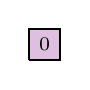
\begin{tikzpicture}[scale=0.4]
\draw[thick, fill=violet!25]  (0,0)--(1,0)--(1,1)--(0,1)--(0,0);
\draw[thick, dotted] (1,0)--(1,1);
\node at (0.5,0.5){$\scriptstyle0 $};
\end{tikzpicture}
}
\qquad
\hackcenter{
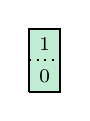
\begin{tikzpicture}[scale=0.4]
\draw[thick, fill=blue!30!green!25]  (0,0)--(1,0)--(1,2)--(0,2)--(0,0);
\draw[thick, dotted] (0,1)--(1,1);
\node at (0.5,0.5){$\scriptstyle0 $};
\node at (0.5,1.5){$\scriptstyle1 $};
\end{tikzpicture}
}
\qquad
\hackcenter{
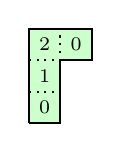
\begin{tikzpicture}[scale=0.4]
\draw[thick, fill=green!20]  (0,-1)--(1,-1)--(1,1)--(2,1)--(2,2)--(0,2)--(0,-1);
\draw[thick, dotted] (0,1)--(1,1)--(1,2);
\draw[thick, dotted] (0,0)--(1,0);
\node at (0.5,-0.5){$\scriptstyle0 $};
\node at (0.5,0.5){$\scriptstyle1 $};
\node at (0.5,1.5){$\scriptstyle2 $};
\node at (1.5,1.5){$\scriptstyle0$};
\end{tikzpicture}
}
\qquad
\hackcenter{
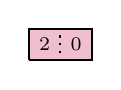
\begin{tikzpicture}[scale=0.4]
\draw[thick, fill=purple!25]  (0,1)--(2,1)--(2,2)--(0,2)--(0,1);
\draw[thick, dotted] (0,1)--(1,1)--(1,2);
\node at (0.5,1.5){$\scriptstyle2 $};
\node at (1.5,1.5){$\scriptstyle0 $};
\end{tikzpicture}
}
\qquad
\hackcenter{
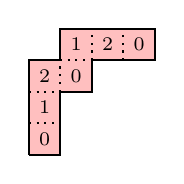
\begin{tikzpicture}[scale=0.4]
\draw[thick, fill=pink]  (0,0)--(1,0)--(1,2)--(2,2)--(2,3)--(4,3)--(4,4)--(1,4)--(1,3)--(0,3)--(0,0);
\draw[thick, dotted] (0,1)--(1,1);
\draw[thick, dotted] (0,2)--(1,2);
\draw[thick, dotted] (0,3)--(2,3);
\draw[thick, dotted] (1,2)--(1,4);
\draw[thick, dotted] (2,3)--(2,4);
\draw[thick, dotted] (3,3)--(3,4);
\node at (0.5,0.5){$\scriptstyle0 $};
\node at (0.5,1.5){$\scriptstyle1 $};
\node at (0.5,2.5){$\scriptstyle2 $};
\node at (1.5,2.5){$\scriptstyle0 $};
\node at (1.5,3.5){$\scriptstyle1 $};
\node at (2.5,3.5){$\scriptstyle2 $};
\node at (3.5,3.5){$\scriptstyle0 $};
\end{tikzpicture}
}
\qquad
\hackcenter{
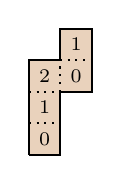
\begin{tikzpicture}[scale=0.4]
\draw[thick,  fill=brown!35]  (0,0)--(1,0)--(1,2)--(2,2)--(2,4)--(1,4)--(1,3)--(0,3)--(0,0);
\draw[thick, dotted] (0,1)--(1,1);
\draw[thick, dotted] (0,2)--(1,2);
\draw[thick, dotted] (0,3)--(2,3);
\draw[thick, dotted] (1,2)--(1,4);
\draw[thick, dotted] (2,3)--(2,4);
\node at (0.5,0.5){$\scriptstyle0 $};
\node at (0.5,1.5){$\scriptstyle1 $};
\node at (0.5,2.5){$\scriptstyle2 $};
\node at (1.5,2.5){$\scriptstyle0 $};
\node at (1.5,3.5){$\scriptstyle1 $};
\end{tikzpicture}
}
\qquad
\cdots
\end{align*}
\caption{Real cuspidal ribbons \(\zeta^{\alpha_0}; \zeta^{\alpha_0 + \alpha_1}; 
\zeta^{\delta + \alpha_0}; \zeta^{\alpha_2 + \alpha_0}; \zeta^{2 \delta + \alpha_0}; \zeta^{\delta + \alpha_0 + \alpha_1}
\)}
\label{fig:BigEx1}       
\end{figure}

At the minimum end of the preorder \(\succeq\), we have the real positive roots:
\begin{align*}
\cdots \succ 2 \delta + \alpha_1 + \alpha_2 \succ \delta+\alpha_2 \succ \delta + \alpha_1 + \alpha_2 \succ \alpha_1 \succ \alpha_1 + \alpha_2 \succ \alpha_2.
\end{align*}
Cuspidal ribbons \(\zeta^\beta\) associated to these roots appear in Figure~\ref{fig:BigEx2}. 
\begin{figure}
\begin{align*}
{}
\cdots
\qquad
\hackcenter{
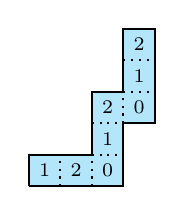
\begin{tikzpicture}[scale=0.4]
\draw[thick, fill=cyan!30] (0,0)--(3,0)--(3,2)--(4,2)--(4,5)--(3,5)--(3,3)--(2,3)--(2,1)--(0,1)--(0,0);
\draw[thick, dotted] (1,0)--(1,1);
\draw[thick, dotted] (2,0)--(2,1);
\draw[thick, dotted] (3,2)--(3,3);
\draw[thick, dotted] (2,1)--(3,1);
\draw[thick, dotted] (2,2)--(3,2);
\draw[thick, dotted] (3,3)--(4,3);
\draw[thick, dotted] (3,4)--(4,4);
\node at (0.5,0.5){$\scriptstyle1 $};
\node at (1.5,0.5){$\scriptstyle2 $};
\node at (2.5,0.5){$\scriptstyle0 $};
\node at (2.5,1.5){$\scriptstyle1 $};
\node at (2.5,2.5){$\scriptstyle2 $};
\node at (3.5,2.5){$\scriptstyle0 $};
\node at (3.5,3.5){$\scriptstyle1 $};
\node at (3.5,4.5){$\scriptstyle2 $};
\end{tikzpicture}
}
\qquad
\hackcenter{
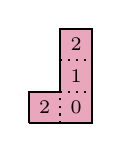
\begin{tikzpicture}[scale=0.4]
\draw[thick, fill=purple!35] (2,2)--(4,2)--(4,5)--(3,5)--(3,3)--(2,3)--(2,2);
\draw[thick, dotted] (3,2)--(3,3);
\draw[thick, dotted] (3,3)--(4,3);
\draw[thick, dotted] (3,4)--(4,4);
\node at (2.5,2.5){$\scriptstyle2 $};
\node at (3.5,2.5){$\scriptstyle0 $};
\node at (3.5,3.5){$\scriptstyle1 $};
\node at (3.5,4.5){$\scriptstyle2 $};
\end{tikzpicture}
}
\qquad
\hackcenter{
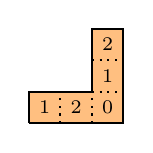
\begin{tikzpicture}[scale=0.4]
\draw[thick, fill=orange!50] (1,2)--(4,2)--(4,5)--(3,5)--(3,3)--(1,3)--(1,2);
\draw[thick, dotted] (2,2)--(2,3);
\draw[thick, dotted] (3,2)--(3,3);
\draw[thick, dotted] (3,3)--(4,3);
\draw[thick, dotted] (3,4)--(4,4);
\node at (1.5,2.5){$\scriptstyle1 $};
\node at (2.5,2.5){$\scriptstyle2 $};
\node at (3.5,2.5){$\scriptstyle0 $};
\node at (3.5,3.5){$\scriptstyle1 $};
\node at (3.5,4.5){$\scriptstyle2 $};
\end{tikzpicture}
}
\qquad
\hackcenter{
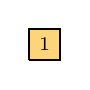
\begin{tikzpicture}[scale=0.4]
\draw[thick, fill=yellow!40!orange!50]  (0,0)--(1,0)--(1,1)--(0,1)--(0,0);
\draw[thick, dotted] (1,0)--(1,1);
\node at (0.5,0.5){$\scriptstyle1 $};
\end{tikzpicture}
}
\qquad
\hackcenter{
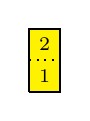
\begin{tikzpicture}[scale=0.4]
\draw[thick, fill=yellow]  (0,0)--(1,0)--(1,2)--(0,2)--(0,0);
\draw[thick, dotted] (0,1)--(1,1);
\node at (0.5,0.5){$\scriptstyle1 $};
\node at (0.5,1.5){$\scriptstyle2 $};
\end{tikzpicture}
}
\qquad
\hackcenter{
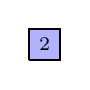
\begin{tikzpicture}[scale=0.4]
\draw[thick, fill=blue!30]  (0,0)--(1,0)--(1,1)--(0,1)--(0,0);
\draw[thick, dotted] (1,0)--(1,1);
\node at (0.5,0.5){$\scriptstyle2 $};
\end{tikzpicture}
}
\end{align*}
\caption{Real cuspidal ribbons \(
\zeta^{2 \delta + \alpha_1 + \alpha_2}; \zeta^{ \delta+\alpha_2}; \zeta^{\delta + \alpha_1 + \alpha_2}; \zeta^{ \alpha_1}; \zeta^{\alpha_1 + \alpha_2}; \zeta^{\alpha_2}
\)}
\label{fig:BigEx2}       
\end{figure}

Smack in the middle of the preorder \(\succeq\) we have the imaginary roots \(m \delta\), all of which are equivalent under \(\succeq\). We have an imaginary cuspidal ribbon \(\zeta^{t}\) of content \(\delta\) associated to each \(t \in \ZZ_3\), as shown in Figure~\ref{fig:BigEx3}. 
\begin{figure}
\begin{align*}
{}
\hackcenter{
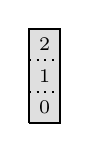
\begin{tikzpicture}[scale=0.4]
\draw[thick, fill=lightgray!50]  (0,0)--(1,0)--(1,3)--(0,3)--(0,0);
\draw[thick, dotted] (0,1)--(1,1);
\draw[thick, dotted] (0,2)--(1,2);
\node at (0.5,0.5){$\scriptstyle0 $};
\node at (0.5,1.5){$\scriptstyle1 $};
\node at (0.5,2.5){$\scriptstyle2 $};
\end{tikzpicture}
}
\qquad
\hackcenter{
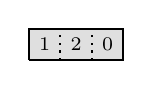
\begin{tikzpicture}[scale=0.4]
\draw[thick, fill=lightgray!50]  (0,0)--(3,0)--(3,1)--(0,1)--(0,0);
\draw[thick, dotted] (1,0)--(1,1);
\draw[thick, dotted] (2,0)--(2,1);
\node at (0.5,0.5){$\scriptstyle1 $};
\node at (1.5,0.5){$\scriptstyle2 $};
\node at (2.5,0.5){$\scriptstyle0 $};
\end{tikzpicture}
}
\qquad
\hackcenter{
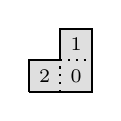
\begin{tikzpicture}[scale=0.4]
\draw[thick, fill=lightgray!50] (0,0)--(2,0)--(2,2)--(1,2)--(1,1)--(0,1)--(0,0);
\draw[thick, dotted] (1,0)--(1,1);
\draw[thick, dotted] (2,0)--(2,1);
\draw[thick, dotted] (1,1)--(2,1);
\node at (0.5,0.5){$\scriptstyle2 $};
\node at (1.5,0.5){$\scriptstyle0 $};
\node at (1.5,1.5){$\scriptstyle1 $};
\end{tikzpicture}
}
\end{align*}
\caption{Imaginary cuspidal ribbons \(
\zeta^{\overline 0}; \zeta^{ \overline 1}; \zeta^{\overline 2}
\)}
\label{fig:BigEx3}     
\end{figure}

If \(\beta \in \Phi_+^\re\), then the unique semicuspidal skew shape of content \(m \beta\) has \(m\) connected components, each of which is identical to the ribbon \(\zeta^\beta\), per Theorem~\textup{7.18}. On the other hand, semicuspidal connected skew shapes of content \(m \delta\) are in bijection with \(\ZZ_3 \times \SSSS_{\tt c}(m)\) via the dilation map, per Proposition~\textup{7.14}. Roughly speaking, for \(t \in \ZZ_3\), one `\(t\)-dilates' the skew shape \(\lambda \in \SSSS_{\tt c}(m)\) by replacing every node in \(\lambda\) with the cuspidal ribbon \(\zeta^{t}\), see \S\textup{7.2}. In Figure~\ref{fig:Infl} an example of this dilation process is depicted.
\begin{figure}
\begin{align*}
{}
\hackcenter{
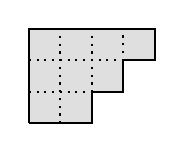
\begin{tikzpicture}[scale=0.4]
\draw[thick, fill=lightgray!50]  (0,0)--(2,0)--(2,1)--(3,1)--(3,2)--(4,2)--(4,3)--(0,3)--(0,0);
\draw[thick, dotted] (0,1)--(2,1);
\draw[thick, dotted] (0,2)--(3,2);
\draw[thick, dotted] (1,0)--(1,3);
\draw[thick, dotted] (2,0)--(2,3);
\draw[thick, dotted] (3,1)--(3,3);
\end{tikzpicture}
}
\;\;\;\;\;
\xrightarrow{\;\;\infl_{\overline 2}\;\;}
\;
\hackcenter{
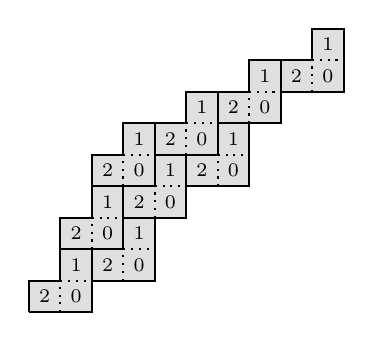
\begin{tikzpicture}[scale=0.4]
\pgfmathsetmacro{\ex}{0}
\pgfmathsetmacro{\ey}{0}
\draw[thick, fill=lightgray!50]  (\ex,\ey)--(\ex+2,\ey)--(\ex+2,\ey+2)--(\ex+1,\ey+2)--(\ex+1,\ey+1)--(\ex,\ey+1)--(\ex,\ey);
\draw[thick, dotted] (\ex+1,\ey)--(\ex+1,\ey+1);
\draw[thick, dotted] (\ex+1,\ey+1)--(\ex+2,\ey+1);
\node at (\ex+0.5,\ey+0.5){$\scriptstyle2 $};
\node at (\ex+1.5,\ey+0.5){$\scriptstyle0 $};
\node at (\ex+1.5,\ey+1.5){$\scriptstyle1 $};
\pgfmathsetmacro{\ex}{2}
\pgfmathsetmacro{\ey}{1}
\draw[thick, fill=lightgray!50]  (\ex,\ey)--(\ex+2,\ey)--(\ex+2,\ey+2)--(\ex+1,\ey+2)--(\ex+1,\ey+1)--(\ex,\ey+1)--(\ex,\ey);
\draw[thick, dotted] (\ex+1,\ey)--(\ex+1,\ey+1);
\draw[thick, dotted] (\ex+1,\ey+1)--(\ex+2,\ey+1);
\node at (\ex+0.5,\ey+0.5){$\scriptstyle2 $};
\node at (\ex+1.5,\ey+0.5){$\scriptstyle0 $};
\node at (\ex+1.5,\ey+1.5){$\scriptstyle1 $};
\pgfmathsetmacro{\ex}{1}
\pgfmathsetmacro{\ey}{2}
\draw[thick, fill=lightgray!50]  (\ex,\ey)--(\ex+2,\ey)--(\ex+2,\ey+2)--(\ex+1,\ey+2)--(\ex+1,\ey+1)--(\ex,\ey+1)--(\ex,\ey);
\draw[thick, dotted] (\ex+1,\ey)--(\ex+1,\ey+1);
\draw[thick, dotted] (\ex+1,\ey+1)--(\ex+2,\ey+1);
\node at (\ex+0.5,\ey+0.5){$\scriptstyle2 $};
\node at (\ex+1.5,\ey+0.5){$\scriptstyle0 $};
\node at (\ex+1.5,\ey+1.5){$\scriptstyle1 $};
\pgfmathsetmacro{\ex}{2}
\pgfmathsetmacro{\ey}{4}
\draw[thick, fill=lightgray!50]  (\ex,\ey)--(\ex+2,\ey)--(\ex+2,\ey+2)--(\ex+1,\ey+2)--(\ex+1,\ey+1)--(\ex,\ey+1)--(\ex,\ey);
\draw[thick, dotted] (\ex+1,\ey)--(\ex+1,\ey+1);
\draw[thick, dotted] (\ex+1,\ey+1)--(\ex+2,\ey+1);
\node at (\ex+0.5,\ey+0.5){$\scriptstyle2 $};
\node at (\ex+1.5,\ey+0.5){$\scriptstyle0 $};
\node at (\ex+1.5,\ey+1.5){$\scriptstyle1 $};
\pgfmathsetmacro{\ex}{3}
\pgfmathsetmacro{\ey}{3}
\draw[thick, fill=lightgray!50]  (\ex,\ey)--(\ex+2,\ey)--(\ex+2,\ey+2)--(\ex+1,\ey+2)--(\ex+1,\ey+1)--(\ex,\ey+1)--(\ex,\ey);
\draw[thick, dotted] (\ex+1,\ey)--(\ex+1,\ey+1);
\draw[thick, dotted] (\ex+1,\ey+1)--(\ex+2,\ey+1);
\node at (\ex+0.5,\ey+0.5){$\scriptstyle2 $};
\node at (\ex+1.5,\ey+0.5){$\scriptstyle0 $};
\node at (\ex+1.5,\ey+1.5){$\scriptstyle1 $};
\pgfmathsetmacro{\ex}{4}
\pgfmathsetmacro{\ey}{5}
\draw[thick, fill=lightgray!50]  (\ex,\ey)--(\ex+2,\ey)--(\ex+2,\ey+2)--(\ex+1,\ey+2)--(\ex+1,\ey+1)--(\ex,\ey+1)--(\ex,\ey);
\draw[thick, dotted] (\ex+1,\ey)--(\ex+1,\ey+1);
\draw[thick, dotted] (\ex+1,\ey+1)--(\ex+2,\ey+1);
\node at (\ex+0.5,\ey+0.5){$\scriptstyle2 $};
\node at (\ex+1.5,\ey+0.5){$\scriptstyle0 $};
\node at (\ex+1.5,\ey+1.5){$\scriptstyle1 $};
\pgfmathsetmacro{\ex}{5}
\pgfmathsetmacro{\ey}{4}
\draw[thick, fill=lightgray!50]  (\ex,\ey)--(\ex+2,\ey)--(\ex+2,\ey+2)--(\ex+1,\ey+2)--(\ex+1,\ey+1)--(\ex,\ey+1)--(\ex,\ey);
\draw[thick, dotted] (\ex+1,\ey)--(\ex+1,\ey+1);
\draw[thick, dotted] (\ex+1,\ey+1)--(\ex+2,\ey+1);
\node at (\ex+0.5,\ey+0.5){$\scriptstyle2 $};
\node at (\ex+1.5,\ey+0.5){$\scriptstyle0 $};
\node at (\ex+1.5,\ey+1.5){$\scriptstyle1 $};
\pgfmathsetmacro{\ex}{6}
\pgfmathsetmacro{\ey}{6}
\draw[thick, fill=lightgray!50]  (\ex,\ey)--(\ex+2,\ey)--(\ex+2,\ey+2)--(\ex+1,\ey+2)--(\ex+1,\ey+1)--(\ex,\ey+1)--(\ex,\ey);
\draw[thick, dotted] (\ex+1,\ey)--(\ex+1,\ey+1);
\draw[thick, dotted] (\ex+1,\ey+1)--(\ex+2,\ey+1);
\node at (\ex+0.5,\ey+0.5){$\scriptstyle2 $};
\node at (\ex+1.5,\ey+0.5){$\scriptstyle0 $};
\node at (\ex+1.5,\ey+1.5){$\scriptstyle1 $};
\pgfmathsetmacro{\ex}{8}
\pgfmathsetmacro{\ey}{7}
\draw[thick, fill=lightgray!50]  (\ex,\ey)--(\ex+2,\ey)--(\ex+2,\ey+2)--(\ex+1,\ey+2)--(\ex+1,\ey+1)--(\ex,\ey+1)--(\ex,\ey);
\draw[thick, dotted] (\ex+1,\ey)--(\ex+1,\ey+1);
\draw[thick, dotted] (\ex+1,\ey+1)--(\ex+2,\ey+1);
\node at (\ex+0.5,\ey+0.5){$\scriptstyle2 $};
\node at (\ex+1.5,\ey+0.5){$\scriptstyle0 $};
\node at (\ex+1.5,\ey+1.5){$\scriptstyle1 $};
\end{tikzpicture}
}
\end{align*}
\caption{\(\overline 2\)-dilation of \(\lambda \in \SSSS_{\tt c}(9)\) into a semicuspidal skew shape \(\infl_{\overline 2}(\lambda)\) of content \(9\delta\)}
\label{fig:Infl}       
\end{figure}

By Theorem~\ref{mainthmcusp}, every skew shape has a unique cuspidal Kostant tiling. In Figure~\ref{fig:Young3ways}, we take \(\tau_0, \tau_1, \tau_2\) to be the Young diagrams associated with the partition \((6,5^4,2^2,1)\) and {\em charges} \(0,1,2\) respectively (see \S\ref{otherformsec}).
The unique cuspidal Kostant tiling is shown for each. Per Theorem~\textup{7.19}, the unique semicuspidal strict Kostant tiling is achieved by choosing tiles to be unions of same-content cuspidal tiles.

\begin{figure}
\begin{align*}
{}
\hackcenter{
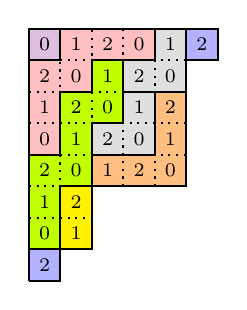
\begin{tikzpicture}[scale=0.4]
\draw[thick, fill=lightgray!50]  (0,0)--(1,0)--(1,1)--(2,1)--(2,3)--(5,3)--(5,7)--(6,7)--(6,8)--(0,8)--(0,0);
\draw[thick,  fill=blue!30]  (0,0)--(1,0)--(1,1)--(0,1)--(0,0);
\draw[thick, fill=blue!30]  (5,7)--(6,7)--(6,8)--(5,8)--(5,7);
\draw[thick, fill=lime]  (0,1)--(1,1)--(1,3)--(2,3)--(2,5)--(3,5)--(3,7)--(2,7)--(2,6)--(1,6)--(1,4)--(0,4)--(0,1);
\draw[thick, fill=yellow]  (1,1)--(2,1)--(2,3)--(1,3)--(1,1);
\draw[thick, fill=pink]  (0,4)--(1,4)--(1,6)--(2,6)--(2,7)--(4,7)--(4,8)--(1,8)--(1,7)--(0,7)--(0,4);
\draw[thick, fill=violet!25] (0,7)--(1,7)--(1,8)--(0,8)--(0,7);
\draw[thick, fill=orange!50] (2,3)--(5,3)--(5,6)--(4,6)--(4,4)--(2,4)--(2,3);
\draw[thick, fill=lightgray!50] (2,4)--(4,4)--(4,6)--(3,6)--(3,5)--(2,5)--(2,4);
\draw[thick, fill=lightgray!50] (3,6)--(5,6)--(5,8)--(4,8)--(4,7)--(3,7)--(3,6);
\draw[thick]  (0,0)--(1,0)--(1,1)--(2,1)--(2,3)--(5,3)--(5,7)--(6,7)--(6,8)--(0,8)--(0,0);
\draw[thick, dotted] (0,1)--(1,1);
\draw[thick, dotted] (0,2)--(2,2);
\draw[thick, dotted] (0,3)--(2,3);
\draw[thick, dotted] (0,4)--(5,4);
\draw[thick, dotted] (0,5)--(5,5);
\draw[thick, dotted] (0,6)--(5,6);
\draw[thick, dotted] (0,7)--(5,7);
\draw[thick, dotted] (1,0)--(1,8);
\draw[thick, dotted] (2,1)--(2,8);
\draw[thick, dotted] (3,3)--(3,8);
\draw[thick, dotted] (4,3)--(4,8);
\draw[thick, dotted] (5,3)--(5,8);
\node at (0.5,7.5){$\scriptstyle 0$};
\node at (1.5,7.5){$\scriptstyle 1$};
\node at (2.5,7.5){$\scriptstyle 2$};
\node at (3.5,7.5){$\scriptstyle 0$};
\node at (4.5,7.5){$\scriptstyle 1$};
\node at (5.5,7.5){$\scriptstyle 2$};
\node at (0.5,6.5){$\scriptstyle 2$};
\node at (1.5,6.5){$\scriptstyle 0$};
\node at (2.5,6.5){$\scriptstyle 1$};
\node at (3.5,6.5){$\scriptstyle 2$};
\node at (4.5,6.5){$\scriptstyle 0$};
\node at (0.5,5.5){$\scriptstyle 1$};
\node at (1.5,5.5){$\scriptstyle 2$};
\node at (2.5,5.5){$\scriptstyle 0$};
\node at (3.5,5.5){$\scriptstyle 1$};
\node at (4.5,5.5){$\scriptstyle 2$};
\node at (0.5,4.5){$\scriptstyle 0$};
\node at (1.5,4.5){$\scriptstyle 1$};
\node at (2.5,4.5){$\scriptstyle 2$};
\node at (3.5,4.5){$\scriptstyle 0$};
\node at (4.5,4.5){$\scriptstyle 1$};
\node at (0.5,3.5){$\scriptstyle 2$};
\node at (1.5,3.5){$\scriptstyle 0$};
\node at (2.5,3.5){$\scriptstyle 1$};
\node at (3.5,3.5){$\scriptstyle 2$};
\node at (4.5,3.5){$\scriptstyle 0$};
\node at (0.5,2.5){$\scriptstyle 1$};
\node at (1.5,2.5){$\scriptstyle 2$};
\node at (0.5,1.5){$\scriptstyle 0$};
\node at (1.5,1.5){$\scriptstyle 1$};
\node at (0.5,0.5){$\scriptstyle 2$};
\end{tikzpicture}
}
\qquad
\;\;
\hackcenter{
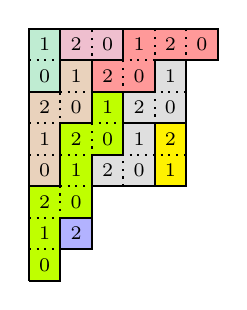
\begin{tikzpicture}[scale=0.4]
\draw[thick, fill=red!40]  (0,0)--(1,0)--(1,1)--(2,1)--(2,3)--(5,3)--(5,7)--(6,7)--(6,8)--(0,8)--(0,0);
\draw[thick, fill=lime]  (0,0)--(1,0)--(1,2)--(2,2)--(2,4)--(3,4)--(3,6)--(2,6)--(2,5)--(1,5)--(1,3)--(0,3)--(0,0);
\draw[thick, fill=blue!30] (1,1)--(2,1)--(2,2)--(1,2)--(1,1);
\draw[thick, fill=lightgray!50] (2,3)--(4,3)--(4,5)--(3,5)--(3,4)--(2,4)--(2,3);
\draw[thick, fill=lightgray!50] (3,5)--(5,5)--(5,7)--(4,7)--(4,6)--(3,6)--(3,5);
\draw[thick, fill=yellow] (4,3)--(5,3)--(5,5)--(4,5)--(4,3);
\draw[thick,  fill=brown!35] (0,3)--(1,3)--(1,5)--(2,5)--(2,7)--(1,7)--(1,6)--(0,6)--(0,3);
\draw[thick, fill=blue!30!green!25] (0,6)--(1,6)--(1,8)--(0,8)--(0,6);
\draw[thick, fill=purple!25] (1,7)--(3,7)--(3,8)--(1,8)--(1,7);
\draw[thick]  (0,0)--(1,0)--(1,1)--(2,1)--(2,3)--(5,3)--(5,7)--(6,7)--(6,8)--(0,8)--(0,0);
\draw[thick, dotted] (0,1)--(1,1);
\draw[thick, dotted] (0,2)--(2,2);
\draw[thick, dotted] (0,3)--(2,3);
\draw[thick, dotted] (0,4)--(5,4);
\draw[thick, dotted] (0,5)--(5,5);
\draw[thick, dotted] (0,6)--(5,6);
\draw[thick, dotted] (0,7)--(5,7);
\draw[thick, dotted] (1,0)--(1,8);
\draw[thick, dotted] (2,1)--(2,8);
\draw[thick, dotted] (3,3)--(3,8);
\draw[thick, dotted] (4,3)--(4,8);
\draw[thick, dotted] (5,3)--(5,8);
\node at (0.5,7.5){$\scriptstyle 1$};
\node at (1.5,7.5){$\scriptstyle 2$};
\node at (2.5,7.5){$\scriptstyle 0$};
\node at (3.5,7.5){$\scriptstyle 1$};
\node at (4.5,7.5){$\scriptstyle 2$};
\node at (5.5,7.5){$\scriptstyle 0$};
\node at (0.5,6.5){$\scriptstyle 0$};
\node at (1.5,6.5){$\scriptstyle 1$};
\node at (2.5,6.5){$\scriptstyle 2$};
\node at (3.5,6.5){$\scriptstyle 0$};
\node at (4.5,6.5){$\scriptstyle 1$};
\node at (0.5,5.5){$\scriptstyle 2$};
\node at (1.5,5.5){$\scriptstyle 0$};
\node at (2.5,5.5){$\scriptstyle 1$};
\node at (3.5,5.5){$\scriptstyle 2$};
\node at (4.5,5.5){$\scriptstyle 0$};
\node at (0.5,4.5){$\scriptstyle 1$};
\node at (1.5,4.5){$\scriptstyle 2$};
\node at (2.5,4.5){$\scriptstyle 0$};
\node at (3.5,4.5){$\scriptstyle 1$};
\node at (4.5,4.5){$\scriptstyle 2$};
\node at (0.5,3.5){$\scriptstyle 0$};
\node at (1.5,3.5){$\scriptstyle 1$};
\node at (2.5,3.5){$\scriptstyle 2$};
\node at (3.5,3.5){$\scriptstyle 0$};
\node at (4.5,3.5){$\scriptstyle 1$};
\node at (0.5,2.5){$\scriptstyle 2$};
\node at (1.5,2.5){$\scriptstyle 0$};
\node at (0.5,1.5){$\scriptstyle 1$};
\node at (1.5,1.5){$\scriptstyle 2$};
\node at (0.5,0.5){$\scriptstyle 0$};
\end{tikzpicture}
}
\qquad
\;\;
\hackcenter{
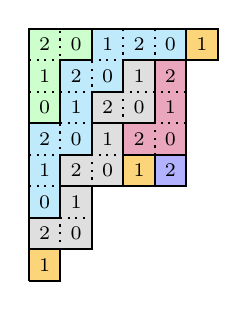
\begin{tikzpicture}[scale=0.4]
\draw[thick,fill=cyan!25]  (0,0)--(1,0)--(1,1)--(2,1)--(2,3)--(5,3)--(5,7)--(6,7)--(6,8)--(0,8)--(0,0);
\draw[thick, fill=lightgray!50] (0,1)--(2,1)--(2,3)--(1,3)--(1,2)--(0,2)--(0,1);
\draw[thick, fill=lightgray!50] (1,3)--(3,3)--(3,5)--(2,5)--(2,4)--(1,4)--(1,3);
\draw[thick, fill=lightgray!50] (2,5)--(4,5)--(4,7)--(3,7)--(3,6)--(2,6)--(2,5);
\draw[thick, fill=green!20] (0,5)--(1,5)--(1,7)--(2,7)--(2,8)--(0,8)--(0,5);
\draw[thick, fill=purple!35] (3,4)--(5,4)--(5,7)--(4,7)--(4,5)--(3,5)--(3,4);
\draw[thick, fill=yellow!40!orange!50] (0,0)--(1,0)--(1,1)--(0,1)--(0,0);
\draw[thick,  fill=yellow!40!orange!50] (5,7)--(6,7)--(6,8)--(5,8)--(5,7);
\draw[thick,  fill=yellow!40!orange!50] (3,3)--(4,3)--(4,4)--(3,4)--(3,3);
\draw[thick, fill=blue!30] (4,3)--(5,3)--(5,4)--(4,4)--(4,3);
\draw[thick]  (0,0)--(1,0)--(1,1)--(2,1)--(2,3)--(5,3)--(5,7)--(6,7)--(6,8)--(0,8)--(0,0);
\draw[thick, dotted] (0,1)--(1,1);
\draw[thick, dotted] (0,2)--(2,2);
\draw[thick, dotted] (0,3)--(2,3);
\draw[thick, dotted] (0,4)--(5,4);
\draw[thick, dotted] (0,5)--(5,5);
\draw[thick, dotted] (0,6)--(5,6);
\draw[thick, dotted] (0,7)--(5,7);
\draw[thick, dotted] (1,0)--(1,8);
\draw[thick, dotted] (2,1)--(2,8);
\draw[thick, dotted] (3,3)--(3,8);
\draw[thick, dotted] (4,3)--(4,8);
\draw[thick, dotted] (5,3)--(5,8);
\node at (0.5,7.5){$\scriptstyle 2$};
\node at (1.5,7.5){$\scriptstyle 0$};
\node at (2.5,7.5){$\scriptstyle 1$};
\node at (3.5,7.5){$\scriptstyle 2$};
\node at (4.5,7.5){$\scriptstyle 0$};
\node at (5.5,7.5){$\scriptstyle 1$};
\node at (0.5,6.5){$\scriptstyle 1$};
\node at (1.5,6.5){$\scriptstyle 2$};
\node at (2.5,6.5){$\scriptstyle 0$};
\node at (3.5,6.5){$\scriptstyle 1$};
\node at (4.5,6.5){$\scriptstyle 2$};
\node at (0.5,5.5){$\scriptstyle 0$};
\node at (1.5,5.5){$\scriptstyle 1$};
\node at (2.5,5.5){$\scriptstyle 2$};
\node at (3.5,5.5){$\scriptstyle 0$};
\node at (4.5,5.5){$\scriptstyle 1$};
\node at (0.5,4.5){$\scriptstyle 2$};
\node at (1.5,4.5){$\scriptstyle 0$};
\node at (2.5,4.5){$\scriptstyle 1$};
\node at (3.5,4.5){$\scriptstyle 2$};
\node at (4.5,4.5){$\scriptstyle 0$};
\node at (0.5,3.5){$\scriptstyle 1$};
\node at (1.5,3.5){$\scriptstyle 2$};
\node at (2.5,3.5){$\scriptstyle 0$};
\node at (3.5,3.5){$\scriptstyle 1$};
\node at (4.5,3.5){$\scriptstyle 2$};
\node at (0.5,2.5){$\scriptstyle 0$};
\node at (1.5,2.5){$\scriptstyle 1$};
\node at (0.5,1.5){$\scriptstyle 2$};
\node at (1.5,1.5){$\scriptstyle 0$};
\node at (0.5,0.5){$\scriptstyle 1$};
\end{tikzpicture}
}
\end{align*}
\caption{Cuspidal Kostant tilings for \(\tau_0, \tau_1, \tau_2\)}
\label{fig:Young3ways}      
\end{figure}
The Kostant partitions associated with these tilings are:
\begin{align*}
\bkap^{\tau_0} &= (\alpha_0  \hspace{-0.5mm} \mid \hspace{-0.5mm} 2\delta+\alpha_0  \hspace{-0.5mm} \mid \hspace{-0.5mm} 2\delta + \alpha_0 + \alpha_1 \hspace{-0.5mm} \mid \hspace{-0.5mm}  \delta^2  \hspace{-0.5mm} \mid \hspace{-0.5mm} \delta + \alpha_1 + \alpha_2  \hspace{-0.5mm} \mid \hspace{-0.5mm} \alpha_1 + \alpha_2  \hspace{-0.5mm} \mid \hspace{-0.5mm} \alpha_2^2);\\
\bkap^{\tau_1} &= (\alpha_0 + \alpha_1  \hspace{-0.5mm} \mid \hspace{-0.5mm} \alpha_2 + \alpha_0  \hspace{-0.5mm} \mid \hspace{-0.5mm} \delta + \alpha_0 + \alpha_1  \hspace{-0.5mm} \mid \hspace{-0.5mm} \delta + \alpha_2 + \alpha_0  \hspace{-0.5mm} \mid \hspace{-0.5mm} 2\delta + \alpha_0 + \alpha_1  \hspace{-0.5mm} \mid \hspace{-0.5mm}  \delta^2  \hspace{-0.5mm} \mid \hspace{-0.5mm} \alpha_1 + \alpha_2  \hspace{-0.5mm} \mid \hspace{-0.5mm} \alpha_2);\\
\bkap^{\tau_2} &= (\delta + \alpha_0  \hspace{-0.5mm} \mid \hspace{-0.5mm} 3\delta + \alpha_0  \hspace{-0.5mm} \mid \hspace{-0.5mm}  \delta^3  \hspace{-0.5mm} \mid \hspace{-0.5mm} \delta + \alpha_2  \hspace{-0.5mm} \mid \hspace{-0.5mm} \alpha_1^3  \hspace{-0.5mm} \mid \hspace{-0.5mm} \alpha_2).
\end{align*}
By Theorem~\ref{mainthmcusp}, these Kostant partitions are bilexicographically maximal amongst all Kostant partitions induced by Kostant tilings for \(\tau_0, \tau_1, \tau_2\), respectively. 
\end{exam}

\subsection{ArXiv Version}\label{SS:ArxivVersion}  In order to keep the paper from becoming overlong we chose to relegate several of the more routine calculations to the \texttt{arXiv} version of the paper.  The reader interested in seeing these additional details can download the \LaTeX~source file from the \texttt{arXiv}.  Near the beginning of the file is a toggle which allows one to compile the paper with these calculations included.

\section{Ribbons and skew shapes}\label{skewshapesec}
We introduce the main combinatorial objects in this section. Many results in this section are well known, but we include full proofs for clarity, as some of our terminology and setup is new. 
We denote the set of integers by \(\Z\), the natural numbers \(\NN = \{1,2,\ldots,\}\), and use the shorthand \([a,b] = \{a, a+1, \ldots, b\}\) for all \(a\leq b \in \Z\).

\subsection{Nodes}
Let \(\N = \Z \times \Z\). We refer to elements of \(\N\) as {\em nodes}. By convention, we visually represent nodes as boxes in a \(\Z \times \Z\) `matrix', so that the node \((i,j)\) is a box in the \(i\)th row and \(j\)th column of the array. In this orientation, positive increase in the first component corresponds to a southward move in the array, and positive increase in the second component corresponds to an eastward move in the array. For \(u \in \N\), we will write \(u_1, u_2\) for the components of \(u\), so that \(u = (u_1, u_2)\). We treat \(\N\) as a \(\ZZ\)-module, so that
\begin{align*}
n(u_1, u_2) = (nu_1, nu_2), \qquad \textup{ and } \qquad (u_1,u_2) +(v_1, v_2) = (u_1 + v_1, u_2 + v_2).
\end{align*}






\subsection{Translation}
For \(c \in \N\), we define the {\em translation by \(c\)} map \(\T_c:\N \to \N\) by \(\T_cu = 
u+ c\) for all \(u \in \N\). If \(\tau \subset \N\), we define \(\T_c \tau = \{\T_c u \mid u \in \tau\}\).
We define the special single-unit north, east, south and west translations \(\no, \ea, \so, \we\) by setting 
\begin{align*}
\no := \T_{(-1,0)},\qquad \ea := \T_{(0,1)},\qquad \so := \T_{(1,0)},\qquad \we  := \T_{(0,-1)}.
\end{align*}


\subsection{Relations between nodes}
We define transitive relations \(\searrow, \SEarrow, \nearrow, \NEarrow\) on \(\N\) by
\begin{align*}
u \searrow v &\iff v = \so^k \ea^\ell u \textup{ for some }k,\ell \in \ZZ_{\geq 0}.\\
u \SEarrow v &\iff v = \so^k \ea^\ell u \textup{ for some }k,\ell \in \ZZ_{> 0}.\\
u \nearrow v &\iff v = \no^k \ea^\ell u \textup{ for some }k,\ell \in \ZZ_{\geq 0}.\\
u \NEarrow v &\iff v = \no^k \ea^\ell u \textup{ for some }k,\ell \in \ZZ_{> 0}.
\end{align*}
We note that \(\searrow, \nearrow\) are in fact partial orders on \(\N\), with \(\searrow\) being the product partial order induced by \(\ZZ\) on \(\N\). 
We extend \(\SEarrow, \NEarrow\) to subsets \(\tau, \nu \subset \N\), writing \(\tau \NEarrow \nu\) provided \(u \NEarrow v\) for all \(u \in \tau, v \in \nu\). 
For \(u \in \tau\subset \N\), we say \(u \in \tau\) is {\em maximally northeast} (resp. {\em maximally southwest}) {\em in} \(\tau\) provided that does not exist any \(u \neq v \in \tau\) such that \(u \nearrow v\) (resp. \(v \nearrow u\)).

\begin{figure}
\begin{align*}
{}
\hackcenter{
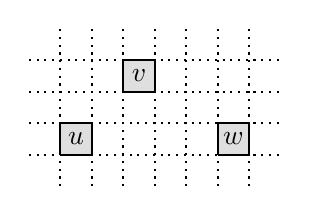
\begin{tikzpicture}[scale=0.4]
\draw[thick, fill = lightgray!50] (0,0)--(1,0)--(1,1)--(0,1)--(0,0);
\draw[thick, fill = lightgray!50] (2,2)--(3,2)--(3,3)--(2,3)--(2,2);
\draw[thick, fill = lightgray!50] (5,0)--(6,0)--(6,1)--(5,1)--(5,0);
\draw[thick, dotted] (-1,0)--(7,0);
\draw[thick, dotted] (-1,1)--(7,1);
\draw[thick, dotted] (-1,2)--(7,2);
\draw[thick, dotted] (-1,3)--(7,3);
\draw[thick, dotted] (0,-1)--(0,4);
\draw[thick, dotted] (1,-1)--(1,4);
\draw[thick, dotted] (2,-1)--(2,4);
\draw[thick, dotted] (3,-1)--(3,4);
\draw[thick, dotted] (4,-1)--(4,4);
\draw[thick, dotted] (5,-1)--(5,4);
\draw[thick, dotted] (6,-1)--(6,4);
\node at (0.5,0.5){$u$};
\node at (2.5,2.5){$v$};
\node at (5.5,0.5){$w$};
\end{tikzpicture}
}
\end{align*}
\caption{Nodes \(u,v,w\), satisfying \(u  \nearrow v\), \(v \searrow w\), \(u \nearrow w\), \(u \searrow w\)}
\label{fig:nodes}     
\end{figure}

For \(u,v \in \N\), a {\em path from \(u\) to \(v\)} is a sequence of nodes \((z^i)_{i=1}^k\) such that \(z^1 = u\), \(z^k = v\), and such that \(z^{i+1} \in \{\no(z^i), \ea(z^i), \so(z^i), \we(z^i)\}\) for \(i \in [1,k-1]\). We say it is moreover a \(\no/\ea\) (resp. \(\so/\ea\)) path if \(z^{i+1} \in \{\no(z^i), \ea(z^i)\}\) (resp. \(z^{i+1} \in \{\so(z^i), \ea(z^i)\}\)) for all \(i \in [1,k-1]\). Defining \(\dist(u,v) = |v_1 + v_2 - u_1 -u_2|\), we have that \(\dist(u,v)+1\) is the length of the shortest path from \(u\) to \(v\), and is thus the length of any \(\no/\ea\) or \(\so/\ea\) path that connects \(u\) and \(v\).

For \(u \in \N\), set \(\diag(u) = u_2 - u_1 \in \ZZ\), and define the {\em \(n\)th diagonal} in \(\N\) to be the set
\begin{align*}
\D_n &= \{u \in \N \mid \diag(u) = n\}\\
&= \{(\so \ea)^k(0,n) \mid k \in \ZZ_{\geq 0}\} \cup \{(\no \we)^k(0,n) \mid k \in \ZZ_{>0}\}.
\end{align*}


\subsection{Skew shapes}
Now we define the main combinatorial object of study in this paper.

\begin{defi}\label{skewdef}
We say a finite subset \(\tau\) of \(\N\) is:
\begin{enumerate}
\item a {\em skew shape} provided that for all \(u,w \in \tau\), \(v \in \N\), \(u \searrow v \searrow w\) implies \(v \in \tau\).
\item {\em thin} if \(|\D_n \cap \tau| \leq 1\) for all \(n \in \N\).
\item {\em connected} if for all \(u,v \in \tau\), there exists a path from \(u\) to \(v\) contained in \(\tau\).
\item a {\em ribbon} provided that \(\tau\) is a nonempty thin connected skew shape.
\item {\em cornered} if there exists at most one \(u \in \tau\) such that \(\so u, \we u \notin \tau\) and at most one \(v \in \tau\) such that \(\no v, \ea v \notin \tau\).
\item {\em diagonal-convex} provided that for all \(n \in \NN\), \(u,w \in \D_n \cap \tau\), and \(v \in \D_n\), \(u \searrow v \searrow w\) implies \(v \in \tau\).
\item a {\em Young diagram} provided that \(\tau = \varnothing\) or \(\tau\) is a skew shape containing a node \(\tau_{\nnww}\) such that \(\tau_{\nnww} \searrow u\) for all \(u \in \tau\).
\end{enumerate}
We write \(\SSSS\) (resp. \(\SSSS_{\tt c}\)) for the set of all skew shapes (resp. nonempty connected skew shapes), and \(\SSSS(n)\) (resp. \(\SSSS_{\tt c}(n)\)) for the subset of those of cardinality \(n\).
\end{defi}


\begin{figure}
\begin{align*}
{}
\hackcenter{
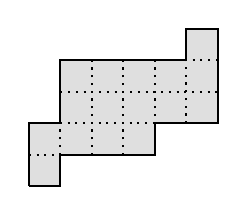
\begin{tikzpicture}[scale=0.4]
\draw[thick, fill=lightgray!50]  (0,-1)--(1,-1)--(1,0)--(4,0)--(4,1)--(6,1)--(6,4)--(5,4)--(5,3)--(1,3)--(1,2)--(1,1)--(0,1)--(0,-1);
\draw[thick, dotted] (1,0)--(1,1);
\draw[thick, dotted] (2,0)--(2,3);
\draw[thick, dotted] (3,0)--(3,3);
\draw[thick, dotted] (4,0)--(4,3);
\draw[thick, dotted] (5,1)--(5,3);
\draw[thick, dotted] (0,0)--(4,0);
\draw[thick, dotted] (0,1)--(6,1);
\draw[thick, dotted] (1,2)--(6,2);
\draw[thick, dotted] (2,3)--(6,3);
\draw[thick]  (0,-1)--(1,-1)--(1,0)--(4,0)--(4,1)--(6,1)--(6,4)--(5,4)--(5,3)--(1,3)--(1,2)--(1,1)--(0,1)--(0,-1);
\end{tikzpicture}
}
\qquad
\qquad
\hackcenter{
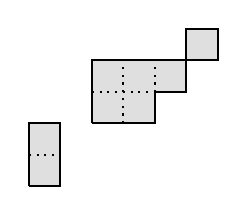
\begin{tikzpicture}[scale=0.4]
\draw[thick, fill=lightgray!50]  (0,-1)--(1,-1)--(1,1)--(0,1)--(0,-1);
\draw[thick, fill=lightgray!50] (2,1)--(4,1)--(4,2)--(5,2)--(5,3)--(2,3)--(2,1);
\draw[thick, fill=lightgray!50] (5,3)--(6,3)--(6,4)--(5,4)--(5,3);
\draw[thick, dotted] (2,1)--(2,3);
\draw[thick, dotted] (3,1)--(3,3);
\draw[thick, dotted] (4,1)--(4,3);
\draw[thick, dotted] (0,0)--(1,0);
\draw[thick, dotted] (2,2)--(5,2);
\draw[thick]  (0,-1)--(1,-1)--(1,1)--(0,1)--(0,-1);
\draw[thick] (2,1)--(4,1)--(4,2)--(5,2)--(5,3)--(2,3)--(2,1);
\draw[thick] (5,3)--(6,3)--(6,4)--(5,4)--(5,3);
\end{tikzpicture}
}
\qquad
\qquad
\hackcenter{
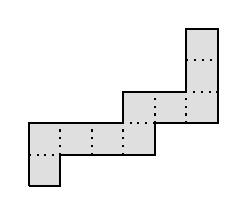
\begin{tikzpicture}[scale=0.4]
\draw[thick, fill=lightgray!50]  (0,-1)--(1,-1)--(1,0)--(4,0)--(4,1)--(6,1)--(6,4)--(5,4)--(5,2)--(3,2)--(3,1)--(1,1)--(0,1)--(0,-1);
\draw[thick, dotted] (1,0)--(1,1);
\draw[thick, dotted] (2,0)--(2,1);
\draw[thick, dotted] (3,0)--(3,1);
\draw[thick, dotted] (4,1)--(4,2);
\draw[thick, dotted] (5,1)--(5,2);
\draw[thick, dotted] (0,0)--(4,0);
\draw[thick, dotted] (0,1)--(6,1);
\draw[thick, dotted] (3,2)--(6,2);
\draw[thick, dotted] (5,3)--(6,3);
\draw[thick]  (0,-1)--(1,-1)--(1,0)--(4,0)--(4,1)--(6,1)--(6,4)--(5,4)--(5,2)--(3,2)--(3,1)--(1,1)--(0,1)--(0,-1);
\end{tikzpicture}
}
\end{align*}
\caption{Connected skew shape; disconnected skew shape; ribbon}
\label{fig:examples}      
\end{figure}


\begin{rema}\label{YDrem1}
Ribbons are also variously called {\em skew hooks}, {\em rim hooks} or {\em edge hooks} in the literature. Every skew shape can be realized as a set difference \(\lambda/ \mu := \lambda \backslash \mu\) of Young diagrams, and, in such context, are often called {\em skew Young diagrams}. We discuss this connection further in \S\ref{otherformsec}.
\end{rema}

\subsection{Basic lemmas on skew shapes}
We record some fundamental lemmas on skew shapes in this section. The proofs are routine, so we omit them here. Full details can be found in the \texttt{arXiv} version of the paper as explained in \S\ref{SS:ArxivVersion}. 

\begin{lemma}\label{skew:cornered=connected}
Let \(\tau\) be a skew shape. Then \(\tau\) is cornered if and only if \(\tau\) is connected.
\end{lemma}


\begin{lemma}\label{CSS=PDC}
Let \(\tau\) be a finite subset of \(\N\). Then \(\tau\) is a connected skew shape if and only if \(\tau\) is cornered and diagonal-convex.
\end{lemma}


\begin{lemma}\label{pathcrit}
Let \(\tau\) be a finite subset of \(\N\). Then \(\tau\) is a connected skew shape if and only if every \(u,v \in \tau\) satisfies:
\begin{enumerate}
\item If \(u \searrow v\), then every \(\so/\ea\) path from \(u\) to \(v\) is contained in \(\tau\);
\item If \(u \nearrow v\), then there exists a \(\no/\ea\) path from \(u\) to \(v\) contained in \(\tau\).
\end{enumerate}
\end{lemma}


\subsubsection{Connected components}
Any nonempty finite set \(\tau \subseteq \N\) may be decomposed into {\em connected components}, i.e., nonempty connected sets \(\tau_1, \ldots, \tau_k\) for some \(k \in \NN\), such that there is no path from \(u\) to \(v\) contained in \(\tau\) whenever \(u \in \tau_i, v \in \tau_j\) for \(i \neq j\).

\begin{lemma}\label{seconnect}
Let \(\tau \in \SSSS\), and \(u,v \in \tau\) be such that \(u \searrow v\). Then the nodes \(\{w \in \N \mid u \searrow w \searrow v\}\) belong to the same connected component of \(\tau\).
\end{lemma}


\begin{lemma}\label{skewcomps}
Connected components of skew shapes are connected skew shapes.
\end{lemma}



\begin{lemma}\label{skewshapecondecomp}
Let \(\tau\) be a nonempty finite subset of \(\N\). Then \(\tau \in \SSSS\) if and only if there exists some \(k \in \NN\) and \(\tau_k \NEarrow \cdots \NEarrow \tau_1 \in \SSSS_{\tt c}\) such that \(\tau = \tau_1 \sqcup \cdots \sqcup \tau_k\).
\end{lemma}


\begin{lemma}\label{uniquemax}
Let \(\tau\) be a nonempty skew shape. Then there exists a unique maximally southwest node \(u \in \tau\), a unique maximally northeast node \(v \in \tau\), and \(u \nearrow w \nearrow v\) for all \(w \in \tau\).
\end{lemma}

In view of Lemma~\ref{uniquemax}, for a nonempty skew shape \(\tau\), we may give the unique maximally southwest (resp. northeast) element the label \(\tau_{\ssww}\) (resp. \(\tau_{\nnee}\)). 

\subsubsection{Basic lemmas on ribbons}

\begin{lemma}\label{dumbdiag}
Let \((z^i)_{i = 1}^k\) be a \(\no/\ea\) path. Then \(\diag(z^i) = \diag(z^1) + i -1\) for \(i \in [1,k]\).
\end{lemma}

\begin{lemma}\label{hookispath}
Let \(\xi\) be a finite subset of \(\N\). Then \(\xi\) is a ribbon if and only if there exists a \(\no/\ea\) path  \((z^i)_{i = 1}^{|\xi|}\) such that \(\xi = \{z^i\}_{i = 1}^{|\xi|}\).
\end{lemma}

\begin{lemma}\label{sizehook}
For a ribbon \(\xi\), we have \(|\xi| = \dist(\xi_{\ssww}, \xi_{\nnee})+1\).
\end{lemma}


\subsection{Tilings and tableaux}\label{tilingsec}
Let \(\tau\) be a nonempty skew shape. A {\em tiling} of \(\tau\) is a set \(\Lambda\) of pairwise disjoint nonempty skew shapes such that \(\tau = \bigsqcup_{\lambda \in \Lambda} \lambda\). We call the members of \(\Lambda\) {\em tiles}.
A {\em \(\Lambda\)-tableau} \(\ttt\) is a bijection \(\ttt: [1, |\Lambda|] \to \Lambda\) such that \(u \in \ttt(i), v \in \ttt(j)\) and \(u \searrow v\) imply \(i\leq j\). We also refer to the pair \((\Lambda, \ttt)\), or the tile sequence \((\ttt(1), \ldots, \ttt(|\Lambda|))\), as a {\em tableau for \(\tau\)}.
Roughly speaking, the ordering condition means the tiles \(\ttt(1), \ldots, \ttt(|\Lambda|)\) can be sequentially `slid into place' from the southeast without their constituent boxes colliding. For instance, in Figure~\ref{fig:tilex}, a tiling \(\Lambda\) for a skew shape \(\tau\) is shown, along with the (only) two possible \(\Lambda\)-tableaux. 

\begin{figure}
\begin{align*}
{}
\hackcenter{
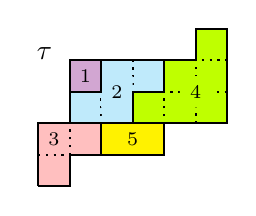
\begin{tikzpicture}[scale=0.4]
\draw[thick, fill=violet!35]   (0,-1)--(1,-1)--(1,0)--(4,0)--(4,1)--(6,1)--(6,4)--(5,4)--(5,3)--(1,3)--(1,2)--(1,1)--(0,1)--(0,-1);
\draw[thick, fill=pink]  (0,-1)--(1,-1)--(1,0)--(2,0)--(2,1)--(1,1)--(0,1)--(0,-1);
\draw[thick, fill=yellow] (2,0)--(4,0)--(4,1)--(2,1)--(2,0);
\draw[thick,fill=lime] (3,1)--(6,1)--(6,4)--(5,4)--(5,3)--(4,3)--(4,2)--(3,2)--(3,1);
\draw[thick, fill=cyan!25] (1,1)--(3,1)--(3,2)--(4,2)--(4,3)--(2,3)--(2,2)--(1,2)--(1,1);
\draw[thick, dotted] (1,0)--(1,1);
\draw[thick, dotted] (2,0)--(2,3);
\draw[thick, dotted] (3,0)--(3,3);
\draw[thick, dotted] (4,0)--(4,3);
\draw[thick, dotted] (5,1)--(5,3);
\draw[thick, dotted] (0,0)--(4,0);
\draw[thick, dotted] (0,1)--(6,1);
\draw[thick, dotted] (1,2)--(6,2);
\draw[thick, dotted] (2,3)--(6,3);
\node at (1.5,2.5){ $\scriptstyle 1$};
\node at (0.5,0.5){ $\scriptstyle3$};
\fill[fill=cyan!25] (2,1.5)--(3,1.5)--(3,2.5)--(2,2.5)--(2,0);
\node at (2.5,2){ $\scriptstyle2$};
\fill[fill=lime] (4.5,1.5)--(5.5,1.5)--(5.5,2.5)--(4.5,2.5)--(4.5,1.5);
\node at (5,2){ $\scriptstyle4$};
\fill[fill=yellow] (2.5,0)--(3.5,0)--(3.5,1)--(2.5,1)--(2.5,0);
\node at (3,0.5){ $\scriptstyle5$};
\node at (0.2,3.2){ $\tau$};
\draw[thick]   (0,-1)--(1,-1)--(1,0)--(4,0)--(4,1)--(6,1)--(6,4)--(5,4)--(5,3)--(1,3)--(1,2)--(1,1)--(0,1)--(0,-1);
\draw[thick]  (0,-1)--(1,-1)--(1,0)--(2,0)--(2,1)--(1,1)--(0,1)--(0,-1);
\draw[thick] (2,0)--(4,0)--(4,1)--(2,1)--(2,0);
\draw[thick] (3,1)--(6,1)--(6,4)--(5,4)--(5,3)--(4,3)--(4,2)--(3,2)--(3,1);
\draw[thick] (1,1)--(3,1)--(3,2)--(4,2)--(4,3)--(2,3)--(2,2)--(1,2)--(1,1);
\end{tikzpicture}
}
\qquad
\qquad
\hackcenter{
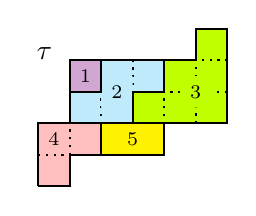
\begin{tikzpicture}[scale=0.4]
\draw[thick, fill=violet!35]   (0,-1)--(1,-1)--(1,0)--(4,0)--(4,1)--(6,1)--(6,4)--(5,4)--(5,3)--(1,3)--(1,2)--(1,1)--(0,1)--(0,-1);
\draw[thick, fill=pink]  (0,-1)--(1,-1)--(1,0)--(2,0)--(2,1)--(1,1)--(0,1)--(0,-1);
\draw[thick, fill=yellow] (2,0)--(4,0)--(4,1)--(2,1)--(2,0);
\draw[thick,fill=lime] (3,1)--(6,1)--(6,4)--(5,4)--(5,3)--(4,3)--(4,2)--(3,2)--(3,1);
\draw[thick, fill=cyan!25] (1,1)--(3,1)--(3,2)--(4,2)--(4,3)--(2,3)--(2,2)--(1,2)--(1,1);
\draw[thick, dotted] (1,0)--(1,1);
\draw[thick, dotted] (2,0)--(2,3);
\draw[thick, dotted] (3,0)--(3,3);
\draw[thick, dotted] (4,0)--(4,3);
\draw[thick, dotted] (5,1)--(5,3);
\draw[thick, dotted] (0,0)--(4,0);
\draw[thick, dotted] (0,1)--(6,1);
\draw[thick, dotted] (1,2)--(6,2);
\draw[thick, dotted] (2,3)--(6,3);
\node at (1.5,2.5){ $\scriptstyle 1$};
\node at (0.5,0.5){ $\scriptstyle4$};
\fill[fill=cyan!25] (2,1.5)--(3,1.5)--(3,2.5)--(2,2.5)--(2,0);
\node at (2.5,2){ $\scriptstyle2$};
\fill[fill=lime] (4.5,1.5)--(5.5,1.5)--(5.5,2.5)--(4.5,2.5)--(4.5,1.5);
\node at (5,2){ $\scriptstyle3$};
\fill[fill=yellow] (2.5,0)--(3.5,0)--(3.5,1)--(2.5,1)--(2.5,0);
\node at (3,0.5){ $\scriptstyle5$};
\node at (0.2,3.2){ $\tau$};
\draw[thick]   (0,-1)--(1,-1)--(1,0)--(4,0)--(4,1)--(6,1)--(6,4)--(5,4)--(5,3)--(1,3)--(1,2)--(1,1)--(0,1)--(0,-1);
\draw[thick]  (0,-1)--(1,-1)--(1,0)--(2,0)--(2,1)--(1,1)--(0,1)--(0,-1);
\draw[thick] (2,0)--(4,0)--(4,1)--(2,1)--(2,0);
\draw[thick] (3,1)--(6,1)--(6,4)--(5,4)--(5,3)--(4,3)--(4,2)--(3,2)--(3,1);
\draw[thick] (1,1)--(3,1)--(3,2)--(4,2)--(4,3)--(2,3)--(2,2)--(1,2)--(1,1);
\end{tikzpicture}
}
\end{align*}
\caption{A tiling \(\Lambda\) for a skew shape \(\tau\), and two \(\Lambda\)-tableaux---label~\(i\) indicates the tile \(\ttt(i)\)}
\label{fig:tilex}       
\end{figure}

\begin{rema}
If \((\Lambda, \ttt)\) is a tableau for \(\tau\) with \(|\lambda| =1\) for all \(\lambda \in \Lambda\), then \((\Lambda, \ttt)\) is a Young tableau in the traditional sense. Young tableaux are important objects in combinatorics, representation theory and algebraic geometry, and the definition above can be viewed as a generalization of Young tableaux to larger tiles.
\end{rema}

\begin{lemma}\label{tabisskew}
Let \((\Lambda, \ttt)\) be a tableau for a skew shape \(\tau\). For \(1 \leq h \leq \ell \leq |\Lambda|\), define \(\tau_{h,\ell} = \bigsqcup_{i = h}^\ell \ttt(i)\). Then \(\tau_{h,\ell}\) is a skew shape.
\end{lemma}
\begin{proof}
Let \(u, w \in \tau_{h,\ell}\), \(v \in \N\), with \(u \searrow v\searrow w\). Then \(u \in \ttt(i)\), \(w \in \ttt(k\)) for some \(i,k \in [h, \ell]\). As \(\tau\) is a skew shape, we have \(v \in \tau\). Then \(v \in \ttt(j)\) for some \(j \in [1, |\Lambda|]\). Since \(u \searrow v\) we have \(h \leq i \leq j\), and since \(v \searrow w\) we have \(j \leq k\leq \ell\). But then \(j \in [h, \ell]\), so \(v \in \tau_{h, \ell}\). Thus \(\tau_{h, \ell}\) is a skew shape.
\end{proof}



\subsection{Removable ribbons}
We say that a skew shape \(\mu \subseteq \tau\) is {\em \(\ssee\)-removable in \(\tau\)} if \(\mu = \tau\) or \((\tau\backslash\mu, \mu)\) is a tableau for \(\tau\). We likewise say that \(\mu\) is {\em \(\nnww\)-removable in \(\tau\)} if \(\mu = \tau\) or \((\mu,\tau\backslash\mu)\) is a tableau for \(\tau\).
Roughly speaking, this means that \(\mu\) is \(\ssee\)-removable if it can be `slid away' to the southeast without colliding with \(\tau\backslash\mu\).
The next lemma follows directly from definitions.
\begin{lemma}\label{remcond}
Let \(\mu \subseteq \tau\) be skew shapes. Then \(\mu\) is \(\ssee\)-removable in \(\tau\) if and only if there does not exist \(u \in \mu\), \(v \in \tau\backslash \mu\) such that \(u \searrow v\). 
\end{lemma}

Let \(\tau\) be a skew shape, and define \(\textup{Rem}_\tau\) to be the set of all pairs \((u,v) \in \tau\) such that
\(u,v\) are in the same connected component of \(\tau\), \(u \nearrow v\), and \(\so u, \ea v \notin \tau\).
Then for \((u,v) \in \textup{Rem}_\tau\), define 
\begin{align*}
\xi^\tau_{u,v} := \{w \in \tau \mid u \nearrow w \nearrow v, \ssee w \notin \tau\} \subseteq \tau.
\end{align*}
An example of the set \(\xi^\tau_{u,v}\) for \((u,v) \in \textup{Rem}_\tau\) is shown in Figure~\ref{fig:xiuvex}. The following lemma is a routine check---full details can be found in the \texttt{arXiv} version of the paper (see \S\ref{SS:ArxivVersion}). 


\begin{figure}
\begin{align*}
{}
\hackcenter{
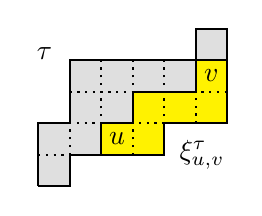
\begin{tikzpicture}[scale=0.4]
\draw[thick, fill=lightgray!50]   (0,-1)--(1,-1)--(1,0)--(4,0)--(4,1)--(6,1)--(6,4)--(5,4)--(5,3)--(1,3)--(1,2)--(1,1)--(0,1)--(0,-1);
\draw[thick, fill=yellow] (2,0)--(4,0)--(4,1)--(6,1)--(6,3)--(5,3)--(5,2)--(3,2)--(3,1)--(2,1)--(2,0);
\draw[thick, dotted] (1,0)--(1,1);
\draw[thick, dotted] (2,0)--(2,3);
\draw[thick, dotted] (3,0)--(3,3);
\draw[thick, dotted] (4,0)--(4,3);
\draw[thick, dotted] (5,1)--(5,3);
\draw[thick, dotted] (0,0)--(4,0);
\draw[thick, dotted] (0,1)--(6,1);
\draw[thick, dotted] (1,2)--(6,2);
\draw[thick, dotted] (2,3)--(6,3);
\draw[thick]   (0,-1)--(1,-1)--(1,0)--(4,0)--(4,1)--(6,1)--(6,4)--(5,4)--(5,3)--(1,3)--(1,2)--(1,1)--(0,1)--(0,-1);
\draw[thick] (2,0)--(4,0)--(4,1)--(6,1)--(6,3)--(5,3)--(5,2)--(3,2)--(3,1)--(2,1)--(2,0);
\node at (0.2,3.2){ $\tau$};
\node at (5.2,0){ $\xi_{u,v}^\tau$};
\node at (2.5,0.5){ $u$};
\node at (5.5,2.5){ $v$};
\end{tikzpicture}
}
\end{align*}
\caption{\(\ssee\)-removable ribbon \(\xi^\tau_{u,v}\) in skew shape \(\tau\)}
\label{fig:xiuvex}       
\end{figure}

\begin{lemma}\label{xiuv}
Let \(\tau\) be a skew shape. Then \(\{ \xi^\tau_{u,v} \mid (u,v) \in \textup{Rem}_\tau\}\) is a complete set of \(\ssee\)-removable ribbons in \(\tau\).
\end{lemma}


 \begin{lemma}\label{remhookswap}
Let \(\tau' \subsetneq \tau\) be skew shapes, let \(u,v,z,w\) be nodes in the same connected component of \(\tau\), and assume \((u,v) \in \textup{Rem}_\tau\), \(\tau' = \tau \backslash \xi^{\tau}_{u,v}\), and \((z,w) \in \textup{Rem}_{\tau'}\). Then we have the following implications:
\begin{enumerate}
\item \(u \nearrow v \nearrow z \nearrow w \implies (u,w) \in \textup{Rem}_{\tau}\); \label{cond:remhookswap1}
\item \(z \nearrow w \nearrow u \nearrow v \implies (z,v) \in \textup{Rem}_\tau\); \label{cond:remhookswap2}
\item \(u \nearrow z \nearrow v \nearrow w \implies (\ssee z, w) \in \textup{Rem}_{\tau}\); \label{cond:remhookswap3}
\item \(z \nearrow u \nearrow w \nearrow v \implies (z, \ssee w) \in \textup{Rem}_{\tau}\); \label{cond:remhookswap4}
\item \(u \nearrow z \nearrow w \nearrow v \implies (\ssee z, \ssee w) \in \textup{Rem}_\tau\); \label{cond:remhookswap5}
\item \(z \nearrow u \nearrow v \nearrow w \implies (z,w) \in \textup{Rem}_\tau\); \label{cond:remhookswap6}
\end{enumerate}
 \end{lemma}
 \begin{proof}
  This is another routine check, with full details included in the \texttt{arXiv} version of the paper (see \S\ref{SS:ArxivVersion}). 
For ease of visualizing these relationships, examples of cases \eqref{cond:remhookswap1}--\eqref{cond:remhookswap6} are shown in Figure~\ref{fig:overlaps}.
\end{proof}


\begin{figure}
\begin{align*}
{}
\hackcenter{
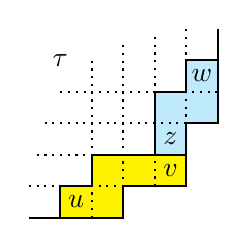
\begin{tikzpicture}[scale=0.4]
\draw[thick]   (1,0)--(2,0);
\draw[thick]   (7,5)--(7,6);
\draw[thick, fill=cyan!25]   (2,0)--(4,0)--(4,1)--(6,1)--(6,3)--(7,3)--(7,5)--(6,5)--(6,4)--(5,4)--(5,2)--(3,2)--(3,1)--(2,1)--(2,0);
\draw[thick, fill=yellow] (2,0)--(4,0)--(4,1)--(6,1)--(6,2)--(3,2)--(3,1)--(2,1)--(2,0);
\draw[thick, dotted] (3,0)--(3,5);
\draw[thick, dotted] (4,0)--(4,5.5);
\draw[thick, dotted] (5,1)--(5,5.75);
\draw[thick, dotted] (6,1)--(6,6);
\draw[thick, dotted] (1,1)--(6,1);
\draw[thick, dotted] (1.25,2)--(6,2);
\draw[thick, dotted] (1.5,3)--(6,3);
\draw[thick, dotted] (2,4)--(7,4);
\draw[thick]   (2,0)--(4,0)--(4,1)--(6,1)--(6,3)--(7,3)--(7,5)--(6,5)--(6,4)--(5,4)--(5,2)--(3,2)--(3,1)--(2,1)--(2,0);
\draw[thick] (2,0)--(4,0)--(4,1)--(6,1)--(6,2)--(3,2)--(3,1)--(2,1)--(2,0);
\node at (2,5){ $\tau$};
\node at (2.5,0.5){ $u$};
\node at (5.5,1.5){ $v$};
\node at (5.5,2.5){ $z$};
\node at (6.5,4.5){ $w$};
\end{tikzpicture}
}
\qquad
\hackcenter{
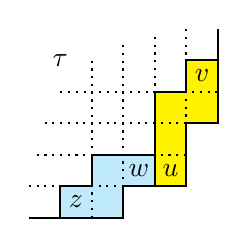
\begin{tikzpicture}[scale=0.4]
\draw[thick]   (1,0)--(2,0);
\draw[thick]   (7,5)--(7,6);
\draw[thick, fill=yellow]   (2,0)--(4,0)--(4,1)--(6,1)--(6,3)--(7,3)--(7,5)--(6,5)--(6,4)--(5,4)--(5,2)--(3,2)--(3,1)--(2,1)--(2,0);
\draw[thick, fill=cyan!25] (2,0)--(4,0)--(4,1)--(5,1)--(5,2)--(3,2)--(3,1)--(2,1)--(2,0);
\draw[thick, dotted] (3,0)--(3,5);
\draw[thick, dotted] (4,0)--(4,5.5);
\draw[thick, dotted] (5,1)--(5,5.75);
\draw[thick, dotted] (6,1)--(6,6);
\draw[thick, dotted] (1,1)--(6,1);
\draw[thick, dotted] (1.25,2)--(6,2);
\draw[thick, dotted] (1.5,3)--(6,3);
\draw[thick, dotted] (2,4)--(7,4);
\draw[thick]   (2,0)--(4,0)--(4,1)--(6,1)--(6,3)--(7,3)--(7,5)--(6,5)--(6,4)--(5,4)--(5,2)--(3,2)--(3,1)--(2,1)--(2,0);
\draw[thick] (2,0)--(4,0)--(4,1)--(5,1)--(5,2)--(3,2)--(3,1)--(2,1)--(2,0);
\node at (2,5){ $\tau$};
\node at (2.5,0.5){ $z$};
\node at (4.5,1.5){ $w$};
\node at (5.5,1.5){ $u$};
\node at (6.5,4.5){ $v$};
\end{tikzpicture}
}
\end{align*}
\begin{align*}
{}
\hackcenter{
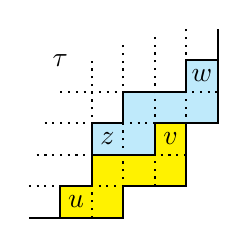
\begin{tikzpicture}[scale=0.4]
\draw[thick]   (1,0)--(2,0);
\draw[thick]   (7,5)--(7,6);
\draw[thick, fill=cyan!25]   (2,0)--(4,0)--(4,1)--(6,1)--(6,3)--(7,3)--(7,5)--(6,5)--(6,4)--(4,4)--(4,3)--(3,3)--(3,1)--(2,1)--(2,0);
\draw[thick, fill=yellow] (2,0)--(4,0)--(4,1)--(6,1)--(6,3)--(5,3)--(5,2)--(3,2)--(3,1)--(2,1)--(2,0);
\draw[thick, dotted] (3,0)--(3,5);
\draw[thick, dotted] (4,0)--(4,5.5);
\draw[thick, dotted] (5,1)--(5,5.75);
\draw[thick, dotted] (6,1)--(6,6);
\draw[thick, dotted] (1,1)--(6,1);
\draw[thick, dotted] (1.25,2)--(6,2);
\draw[thick, dotted] (1.5,3)--(6,3);
\draw[thick, dotted] (2,4)--(7,4);
\draw[thick]   (2,0)--(4,0)--(4,1)--(6,1)--(6,3)--(7,3)--(7,5)--(6,5)--(6,4)--(4,4)--(4,3)--(3,3)--(3,1)--(2,1)--(2,0);
\draw[thick] (2,0)--(4,0)--(4,1)--(6,1)--(6,3)--(5,3)--(5,2)--(3,2)--(3,1)--(2,1)--(2,0);
\node at (2,5){ $\tau$};
\node at (2.5,0.5){ $u$};
\node at (5.5,2.5){ $v$};
\node at (3.5,2.5){ $z$};
\node at (6.5,4.5){ $w$};
\end{tikzpicture}
}
\qquad
\hackcenter{
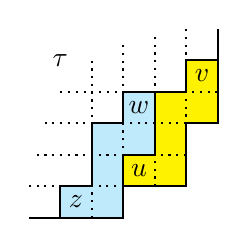
\begin{tikzpicture}[scale=0.4]
\draw[thick]   (1,0)--(2,0);
\draw[thick]   (7,5)--(7,6);
\draw[thick, fill=cyan!25]   (2,0)--(4,0)--(4,1)--(6,1)--(6,3)--(7,3)--(7,5)--(6,5)--(6,4)--(4,4)--(4,3)--(3,3)--(3,1)--(2,1)--(2,0);
\draw[thick, fill=yellow] (4,1)--(6,1)--(6,3)--(7,3)--(7,5)--(6,5)--(6,4)--(5,4)--(5,2)--(4,2)--(4,1);
\draw[thick, dotted] (3,0)--(3,5);
\draw[thick, dotted] (4,0)--(4,5.5); 
\draw[thick, dotted] (5,1)--(5,5.75);
\draw[thick, dotted] (6,1)--(6,6);
\draw[thick, dotted] (1,1)--(6,1);
\draw[thick, dotted] (1.25,2)--(6,2);
\draw[thick, dotted] (1.5,3)--(6,3);
\draw[thick, dotted] (2,4)--(7,4);
\draw[thick] (2,0)--(4,0)--(4,1)--(6,1)--(6,3)--(7,3)--(7,5)--(6,5)--(6,4)--(4,4)--(4,3)--(3,3)--(3,1)--(2,1)--(2,0);
\draw[thick] (4,1)--(6,1)--(6,3)--(7,3)--(7,5)--(6,5)--(6,4)--(5,4)--(5,2)--(4,2)--(4,1);
\node at (2,5){ $\tau$};
\node at (2.5,0.5){ $z$};
\node at (4.5,3.5){ $w$};
\node at (4.5,1.5){ $u$};
\node at (6.5,4.5){ $v$};
\end{tikzpicture}
}
\qquad
\hackcenter{
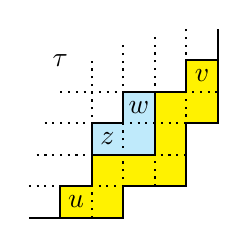
\begin{tikzpicture}[scale=0.4]
\draw[thick]   (1,0)--(2,0);
\draw[thick]   (7,5)--(7,6);
\draw[thick, fill=cyan!25]   (2,0)--(4,0)--(4,1)--(6,1)--(6,3)--(7,3)--(7,5)--(6,5)--(6,4)--(4,4)--(4,3)--(3,3)--(3,1)--(2,1)--(2,0);
\draw[thick, fill=yellow] (3,2)--(3,1)--(2,1)--(2,0)--(4,0)--(4,1)--(6,1)--(6,3)--(7,3)--(7,5)--(6,5)--(6,4)--(5,4)--(5,2)--(4,2)--(3,2);
\draw[thick, dotted] (3,0)--(3,5);
\draw[thick, dotted] (4,0)--(4,5.5); 
\draw[thick, dotted] (5,1)--(5,5.75);
\draw[thick, dotted] (6,1)--(6,6);
\draw[thick, dotted] (1,1)--(6,1);
\draw[thick, dotted] (1.25,2)--(6,2);
\draw[thick, dotted] (1.5,3)--(6,3);
\draw[thick, dotted] (2,4)--(7,4);
\draw[thick] (2,0)--(4,0)--(4,1)--(6,1)--(6,3)--(7,3)--(7,5)--(6,5)--(6,4)--(4,4)--(4,3)--(3,3)--(3,1)--(2,1)--(2,0);
\draw[thick] (3,2)--(3,1)--(2,1)--(2,0)--(4,0)--(4,1)--(6,1)--(6,3)--(7,3)--(7,5)--(6,5)--(6,4)--(5,4)--(5,2)--(4,2)--(3,2);
\node at (2,5){ $\tau$};
\node at (2.5,0.5){ $u$};
\node at (4.5,3.5){ $w$};
\node at (3.5,2.5){ $z$};
\node at (6.5,4.5){ $v$};
\end{tikzpicture}
}
\qquad
\hackcenter{
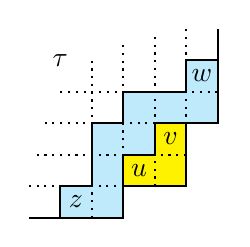
\begin{tikzpicture}[scale=0.4]
\draw[thick]   (1,0)--(2,0);
\draw[thick]   (7,5)--(7,6);
\draw[thick, fill=yellow]   (2,0)--(4,0)--(4,1)--(6,1)--(6,3)--(7,3)--(7,5)--(6,5)--(6,4)--(4,4)--(4,3)--(3,3)--(3,1)--(2,1)--(2,0);
\draw[thick, fill=cyan!25] (2,0)--(4,0)--(4,2)--(5,2)--(5,3)--(7,3)--(7,5)--(6,5)--(6,4)--(4,4)--(4,3)--(3,3)--(3,1)--(2,1)--(2,0);
\draw[thick, dotted] (3,0)--(3,5);
\draw[thick, dotted] (4,0)--(4,5.5); 
\draw[thick, dotted] (5,1)--(5,5.75);
\draw[thick, dotted] (6,1)--(6,6);
\draw[thick, dotted] (1,1)--(6,1);
\draw[thick, dotted] (1.25,2)--(6,2);
\draw[thick, dotted] (1.5,3)--(6,3);
\draw[thick, dotted] (2,4)--(7,4);
\draw[thick]   (2,0)--(4,0)--(4,1)--(6,1)--(6,3)--(7,3)--(7,5)--(6,5)--(6,4)--(4,4)--(4,3)--(3,3)--(3,1)--(2,1)--(2,0);
\draw[thick] (2,0)--(4,0)--(4,2)--(5,2)--(5,3)--(7,3)--(7,5)--(6,5)--(6,4)--(4,4)--(4,3)--(3,3)--(3,1)--(2,1)--(2,0);
\node at (2,5){ $\tau$};
\node at (2.5,0.5){ $z$};
\node at (5.5,2.5){ $v$};
\node at (4.5,1.5){ $u$};
\node at (6.5,4.5){ $w$};
\end{tikzpicture}
}
\end{align*}
\caption{Cases \eqref{cond:remhookswap1}--\eqref{cond:remhookswap6} in Lemma~\ref{remhookswap}}
\label{fig:overlaps}     
\end{figure}


\section{Positive roots and convex preorders}\label{posrootsec}
We fix now and throughout the paper some choice of \(e \in \ZZ_{>1}\). Associated to \(e\) is an affine root system of type \({\tt A}_{e-1}^{(1)}\), corresponding to the affine Dynkin diagram shown in Figure~\ref{fig:dynkin}
(see \cite[\S 4, Table Aff 1]{KacBookInfLie}). This root system plays a crucial role in the representation theory of the Kac-Moody Lie algebra \(\widehat{\mathfrak{sl}}_e\) and its associated quantum group, as well as modular representation theory of the symmetric group.
We describe the root system directly in the sequel.

\begin{figure}
\begin{align*}
{}
\hackcenter{
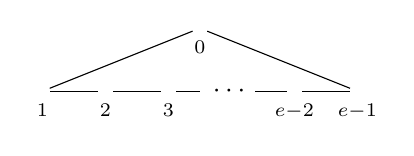
\begin{tikzpicture}[scale=0.4]
\coordinate (0) at (5,1);
\coordinate (1) at (0,-1);
\coordinate (2) at (2,-1);
\coordinate (3) at (4,-1);
\coordinate (4) at (6,-1);
\coordinate (5) at (8,-1);
\coordinate (6) at (10,-1);
\coordinate (0a) at (5,0.9);
\coordinate (1a) at (0,-1.1);
\coordinate (2a) at (2,-1.1);
\coordinate (3a) at (4,-1.1);
\coordinate (4a) at (6,-1.1);
\coordinate (5a) at (8,-1.1);
\coordinate (6a) at (10,-1.1);
\draw [thin, black,shorten <= 0.1cm, shorten >= 0.1cm]   (0) to (1);
\draw [thin, black,shorten <= 0.1cm, shorten >= 0.1cm]   (1) to (2);
\draw [thin, black,shorten <= 0.1cm, shorten >= 0.1cm]   (2) to (3);
\draw [thin, black,shorten <= 0.1cm, shorten >= 0.4cm]   (3) to (4);
\draw [thin, black,shorten <= 0.3cm, shorten >= 0.1cm]   (4) to (5);
\draw [thin, black,shorten <= 0.1cm, shorten >= 0.1cm]   (5) to (6);
\draw [thin, black,shorten <= 0.1cm, shorten >= 0.1cm]   (0) to (6);
\draw (0a) node[below]{$\scriptstyle{0}$};
\draw (1a) node[below]{$\scriptstyle{1}$};
\draw (2a) node[below]{$ \scriptstyle{2}$};
\draw (3a) node[below]{$\scriptstyle{3}$};
\draw (5a) node[below]{$ \scriptstyle{e-2}$};
\draw (6a) node[below]{$\scriptstyle{e-1}$};
\blackdot(5,1);
\blackdot(0,-1);
\blackdot(2,-1);
\blackdot(4,-1);
\blackdot(8,-1);
\blackdot(10,-1);
\draw(6,-1) node{$\cdots$};
\end{tikzpicture}
}
\end{align*}
\caption{Dynkin diagram of type \({\tt A}^{(1)}_{e-1}\)}
\label{fig:dynkin}       
\end{figure}

We write \(\ZZ_e = \ZZ/e\ZZ\), and will indicate elements of \(\ZZ_e\) with barred integers, i.e. \(\overline t = t + e\ZZ\) for \(t \in \ZZ\), freely omitting bars for \(t \in [0,e-1]\) when the context is clear.
Let \(\ZZ I\) be the free \(\ZZ\)-module of rank \(e\), with basis \(I = \{\alpha_i \mid i \in \ZZ_e\}\), and set \(Q_+ = \ZZ_{\geq 0}I\). For \(\beta = \sum_{i \in \Z_e} c_i\alpha_i \in Q_+\), we write \(\height(\beta) := \sum_{i \in \Z_e} c_i \in \ZZ_{\geq 0}\) for the {\em height} of \(\beta\).
For any \(t \in \ZZ_e\), \(h \in \NN\), we define \(\alpha(t,h) \in Q_+\) via
\begin{align*}
\alpha(t,h):= \alpha_t + \alpha_{t+\overline{1}} + \cdots + \alpha_{t+ \overline{h-1}}.
\end{align*}
We have then that \(\height(\alpha(t,h)) = h\). Of particular importance is the {\em null root} of height~\(e\):
\begin{align*}
\delta := \alpha_{ 0} + \cdots + \alpha_{e-1} = \alpha(t,e)\qquad (t \in \ZZ_e).
\end{align*}
It follows from definitions that 
\begin{align}\label{splithookcont}
\alpha(t,h_1 + h_2) = \alpha(t, h_1) + \alpha(t + \overline{h}_1, h_2) 
\end{align}
for all \(t \in \ZZ_e, h_1,h_2 \in \NN\). The element \(\alpha(t,h)\) corresponds to the sum of simple roots in a counterclockwise path of length \(h\) in the Dynkin diagram in Figure~\ref{fig:dynkin} which begins at the vertex labeled \(t\).


\begin{defi} \(\)
\begin{enumerate}
\item
We say \(\beta \in Q_+\) is a {\em positive root} if \(\beta = \alpha(t,h)\) for some \(t \in \ZZ, h \in \NN\). We write \(\Phi_+\) for the set of all positive roots, so we have
\begin{align}
\Phi_+ = \{ \alpha(t,h) \mid t \in \ZZ_e, h \in \NN\} \subset \ZZ I.
\end{align}
\item We say \(\beta \in \Phi_+\) is {\em real} if \(\overline{\height(\beta)} \neq \overline 0\). Writing \(\Phi_+^\re\) for the set of all real positive roots, we have
\begin{align}
\Phi_+^\re =  \{ \alpha(t,h) \mid t \in \ZZ_e, h \in \NN, \overline h \neq \overline 0\} \subset \Phi_+.
\end{align}
\item We say \(\beta \in \Phi_+\) is {\em imaginary} if \(\overline{\height(\beta)} = \overline 0\).  Writing \(\Phi_+^\im\) for the set of imaginary positive roots, we have
\begin{align}\label{allimag}
\Phi_+^\im =  \{ \alpha(t,h) \mid t \in \ZZ_e, h \in \NN, \overline h = \overline 0\} = \{m \delta \mid m \in\NN \} \subset \Phi_+.
\end{align}
\item We say a positive root \(\beta\) is {\em divisible} if there exists \(\beta' \in \Phi_+\), \(m \in \ZZ_{>1}\) such that \(\beta= m \beta'\), and {\em indivisible} if not. Writing \(\Psi\) for the set of indivisible roots, we have
\begin{align}\label{PsiDef}
\Psi = \Phi_+^\re \sqcup \{ \delta\} .
\end{align}
\item We define \(\Phi_+'\) to be the set of all positive integer multiples of positive roots, so we have
\begin{align}\label{multphi}
\Phi_+' = \{m \beta \mid m \in \NN, \beta \in \Phi_+\} = \{m \beta \mid m \in \NN, \beta \in \Psi\} \subset Q_+.
\end{align}
\end{enumerate}
\end{defi}

\subsection{Convex preorders}
A {\em convex preorder} on \(\Phi_+\) is a binary relation \(\succeq\) on \(\Phi_+\) which, for all \(\beta, \gamma, \nu \in \Phi_+\) satisfies the following:
\begin{enumerate}
\item \(\beta \succeq \beta\) (reflexivity); \label{cond:convex1}
\item \(\beta \succeq \gamma\) and \(\gamma \succeq \nu\) imply \(\beta \succeq \nu\) (transitivity); \label{cond:convex2}
\item \(\beta \succeq \gamma\) or \(\gamma \succeq \beta\) (totality); \label{cond:convex3}
\item \(\beta \succeq \gamma\) and \(\beta + \gamma \in \Phi_+\) imply \(\beta \succeq \beta  + \gamma \succeq \gamma\) (convexity); \label{cond:convex4}
\item \(\beta \succeq \gamma\) and \(\gamma \succeq \beta\) if and only if \(\beta = \gamma\) or \(\beta, \gamma \in \Phi_+^\im\) (imaginary equivalency). \label{cond:convex5}
\end{enumerate}
We write \(\beta \succ \gamma\) if \(\beta \succeq \gamma\) and \(\gamma \not \succeq \beta\). Then \eqref{cond:convex3} and \eqref{cond:convex5} together imply that \(\succ\) restricts to a total order on \(\Psi\). We also write \(\beta \approx \gamma\) if \(\beta \succeq \gamma\) and \(\gamma \succeq \beta\), so \eqref{cond:convex5} and (\ref{allimag}) imply that \(\beta \approx \gamma\), \(\beta \neq \gamma\) if and only if \(\beta = m \delta\), \(\gamma = m'\delta\), for some \(m \neq m' \in \NN\). 

\subsection{Examples of convex preorders}
Convex preorders are known to exist for any choice of \(e\), and a classification and general method of construction of convex preorders is given in \cite{ItoClass}. The below proposition, lightly paraphrased from \cite[Example~2.14(ii)]{BaKaTiAffMir} and \cite[Example 3.5]{McNRepKLR3}, provides a low-tech way to generate many distinct convex preorders on \(\Phi_+\).

\begin{prop}\label{genconvex} 
Let \((V, \geq)\) be a totally ordered \(\Q\)-vector space. Let \(h:\ZZ I \to V\) be a \(\ZZ\)-linear map such that \(\beta \mapsto  \frac{h(\beta)}{\textup{ht}(\beta)} \) is injective on \(\Psi \subseteq \ZZ I\). Then the relation 
\begin{align*}
\beta \succeq \gamma \iff \frac{h(\beta)}{\textup{ht}(\beta)} \geq \frac{h(\gamma)}{\textup{ht}(\gamma)}
\end{align*}
defines a convex preorder on \(\Phi_+\).
\end{prop}

One straightforward method (exemplified in \cite[Example 3.6]{McNRepKLR3}) for generating such maps \(h\) as in Proposition~\ref{genconvex} is to 
take \(V=\RR^n\) under the lexicographic order \(\geq\) for some \(n\), and \(\Z\)-linearly extend some set map \(h: I \to V\) such that \(h(\delta)= 0\) and \(h\) is generic in the sense that \(h(\gamma) \notin \QQ_{> 0} h(\beta)\) for distinct \(\beta, \gamma \in \Phi_+\) with \(\textup{ht}(\beta), \textup{ht}(\gamma) < e\).
An example of this approach in the case \(e=3\) appears in Example~\ref{BigEx}. A simpler example is shown next. 

\begin{exam}\label{e2order}
Take \(e=2\). Let \(V = \RR\) under the standard ordering. Define \(h: \ZZ I \to V\) by setting \(h(\alpha_1) = 1\), \(h(\alpha_0) = -1\), and extending by \(\ZZ\)-linearity. Then Proposition~\ref{genconvex} yields the following preorder on \(\Phi_+\):
\begin{align*}
\alpha_1 \succ
\delta+\alpha_1 
\succ
2\delta+\alpha_1
\succ
\cdots
\succ
\ZZ_{>0}\delta
\succ
\cdots
\succ
2\delta+\alpha_0
\succ
\delta+\alpha_0
\succ
\alpha_0.
\end{align*}
This is one of two convex preorders on \(\Phi_+\); the other is the reverse preorder (see \S\ref{revsec}).
\end{exam}

\subsection{Implications of convexity} 
The next lemma follows immediately from definitions:
\begin{lemma}\label{notapprox}
Let \(\beta, \beta' \in \Phi_+\), Then we have:
\begin{enumerate}
\item If \(\beta \approx \beta'\) and \(\height(\beta) > \height(\beta')\), then \(\beta, \beta' \in \Phi_+^\im\); \label{cond:notapprox1}
\item If \(\beta \in \Psi\) and \(\height(\beta) > \height(\beta')\), then \(\beta \not \approx \beta'\); \label{cond:notapprox2}
\item If \(\beta, \beta' \in \Psi\), then \(\beta \approx \beta'\) if and only if \(\beta = \beta'\). \label{cond:notapprox3}
\end{enumerate}
\end{lemma}


We have the following useful generalization of the convexity property:

\begin{lemma} \label{GenConvexLem} \cite{KlCuspSys, BaKaTiAffMir}
Let \(\gamma, \beta_1, \ldots, \beta_k \in \Phi_+\), \(m \in \NN\) be such that \(\beta_1 + \cdots + \beta_k = m \gamma\). Then we have the following:
\begin{enumerate}
\item If \(\gamma \in \Phi_+^\re\), and \(\beta_i \succeq \gamma\) for all \(i \in [1,k]\) or \(\gamma \succeq \beta_i\) for all \(i \in [1,k]\), then \(\gamma = \beta_i\) for all \(i \in [1,k]\). \label{cond:genconvex1}
\item If \(\gamma \in \Phi_+^\im\), and \(\beta_i \succeq \gamma\) for all \(i \in [1,k]\) or \(\gamma \succeq \beta_i\) for all \(i \in [1,k]\), then \(\beta_i \in \Phi_+^\im\) for all \(i \in [1,k]\). \label{cond:genconvex2}
\item If \(\beta_1 \succeq \cdots \succeq \beta_k\), then \(\beta_1 \succeq \gamma \succeq \beta_k\). \label{cond:genconvex3}
\item If \(\beta_1 \succeq \cdots \succeq \beta_k\) and \(\beta_1 \succ \beta_k\), then \(\beta_1 \succ \gamma \succ \beta_k\). \label{cond:genconvex4}
\end{enumerate}
\end{lemma}
\begin{proof}
Claims \eqref{cond:genconvex1} and \eqref{cond:genconvex2} appear as the properties \cite[(Con1), (Con3)]{KlCuspSys}, which follow from \cite[Lemma 3.1]{KlCuspSys}, which utilizes \cite[Lemma 2.9]{BaKaTiAffMir}. Claims \eqref{cond:genconvex3} and \eqref{cond:genconvex4} are contrapositive reformulations implied by \eqref{cond:genconvex1} and \eqref{cond:genconvex2}.
\end{proof}


\begin{lemma} \label{psidef} 
The function \(\NN \times \Psi \to \Phi_+'\), \((n, \beta) \mapsto n \beta\) is a bijection.
\end{lemma}
\begin{proof}
Surjectivity is clear by (\ref{multphi}). For injectivity, assume \(n \beta = n' \beta'\) for some \(n,n' \in \NN\), \(\beta,\beta' \in \Psi\). Then by Lemma~\ref{GenConvexLem} we have \(\beta \approx \beta'\). As \(\beta, \beta' \in \Psi\), this implies that \(\beta = \beta'\) and thus \(n = n'\).
\end{proof}

By Lemma~\ref{psidef} we have well-defined functions \(m:\Phi_+' \to \NN\) and \(\psi: \Phi_+' \to \Psi\) such that \(\gamma = m(\gamma) \psi(\gamma)\) for all \(\gamma \in \Phi_+'\).


\section{Content and cuspidal skew shapes}

\subsection{Content}\label{contentsec}
We define the {\em residue} of a node \(u \in \N\) to be 
\(\res(u) =\overline{u_2 - u_1} = \overline{\diag(u)}\).
The map \(\res: \N \to \Z_e\) is a \(\Z\)-module homomorphism, so we have
\begin{align*}
\res(n u) = n \res(u)
\qquad
\textup{and}
\qquad
\res(u+v) = \res(u) + \res(v),
\end{align*}
for all \(n \in \ZZ\), \(u,v \in \N\). For \(t \in \Z_e\), we write
\begin{align*}
\N_t := \{ u \in \N \mid \res(u) = t\}.
\end{align*}



The {\em content} of a skew shape \(\tau\) is defined as
\begin{align*}
\cont(\tau) = \sum_{u \in \tau} \alpha_{\res(u)} \in Q_+.
\end{align*}
For \(\theta \in Q_+\), we write \(\SSSS(\theta)\) (resp. \(\SSSS_{\tt c}(\theta)\)) for the set of skew shapes (resp. nonempty connected skew shapes) of content \(\theta\). It is clear from definitions then that if \(\Lambda\) is any tiling of \(\tau\), we have
\(
\cont(\tau) = \sum_{\lambda \in \Lambda} \cont(\lambda).
\)
In our visual representation, we label each node with its associated residue. See Figure~\ref{fig:e4con} for examples.

\begin{figure}
\begin{align*}
{}
\hackcenter{
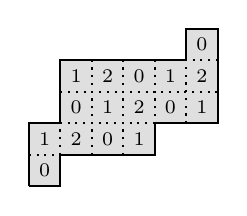
\begin{tikzpicture}[scale=0.4]
\draw[thick, fill=lightgray!50]  (0,-1)--(1,-1)--(1,0)--(4,0)--(4,1)--(6,1)--(6,4)--(5,4)--(5,3)--(1,3)--(1,2)--(1,1)--(0,1)--(0,-1);
\draw[thick, dotted] (1,0)--(1,1);
\draw[thick, dotted] (2,0)--(2,3);
\draw[thick, dotted] (3,0)--(3,3);
\draw[thick, dotted] (4,0)--(4,3);
\draw[thick, dotted] (5,1)--(5,3);
\draw[thick, dotted] (0,0)--(4,0);
\draw[thick, dotted] (0,1)--(6,1);
\draw[thick, dotted] (1,2)--(6,2);
\draw[thick, dotted] (2,3)--(6,3);
\draw[thick]   (0,-1)--(1,-1)--(1,0)--(4,0)--(4,1)--(6,1)--(6,4)--(5,4)--(5,3)--(1,3)--(1,2)--(1,1)--(0,1)--(0,-1);
\node at (0.5,-0.5){$\scriptstyle0 $};
\node at (0.5,0.5){$\scriptstyle1 $};
\node at (1.5,0.5){$\scriptstyle2 $};
\node at (2.5,0.5){$\scriptstyle0 $};
\node at (3.5,0.5){$\scriptstyle1 $};
\node at (1.5,1.5){$\scriptstyle0 $};
\node at (2.5,1.5){$\scriptstyle1 $};
\node at (3.5,1.5){$\scriptstyle2 $};
\node at (4.5,1.5){$\scriptstyle0 $};
\node at (5.5,1.5){$\scriptstyle1 $};
\node at (1.5,2.5){$\scriptstyle1 $};
\node at (2.5,2.5){$\scriptstyle2 $};
\node at (3.5,2.5){$\scriptstyle0 $};
\node at (4.5,2.5){$\scriptstyle1 $};
\node at (5.5,2.5){$\scriptstyle2 $};
\node at (5.5,3.5){$\scriptstyle0 $};
\end{tikzpicture}
}
\qquad
\qquad
\hackcenter{
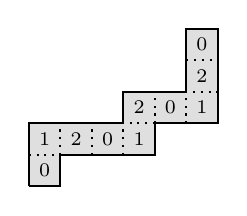
\begin{tikzpicture}[scale=0.4]
\draw[thick, fill=lightgray!50]  (0,-1)--(1,-1)--(1,0)--(4,0)--(4,1)--(6,1)--(6,4)--(5,4)--(5,2)--(3,2)--(3,1)--(1,1)--(0,1)--(0,-1);
\draw[thick, dotted] (1,0)--(1,1);
\draw[thick, dotted] (2,0)--(2,1);
\draw[thick, dotted] (3,0)--(3,1);
\draw[thick, dotted] (4,1)--(4,2);
\draw[thick, dotted] (5,1)--(5,2);
\draw[thick, dotted] (0,0)--(4,0);
\draw[thick, dotted] (0,1)--(6,1);
\draw[thick, dotted] (3,2)--(6,2);
\draw[thick, dotted] (5,3)--(6,3);
\draw[thick]  (0,-1)--(1,-1)--(1,0)--(4,0)--(4,1)--(6,1)--(6,4)--(5,4)--(5,2)--(3,2)--(3,1)--(1,1)--(0,1)--(0,-1);
\node at (0.5,-0.5){$\scriptstyle0 $};
\node at (0.5,0.5){$\scriptstyle1 $};
\node at (1.5,0.5){$\scriptstyle2 $};
\node at (2.5,0.5){$\scriptstyle0 $};
\node at (3.5,0.5){$\scriptstyle1 $};
\node at (3.5,1.5){$\scriptstyle2 $};
\node at (4.5,1.5){$\scriptstyle0 $};
\node at (5.5,1.5){$\scriptstyle1 $};
\node at (5.5,2.5){$\scriptstyle2 $};
\node at (5.5,3.5){$\scriptstyle0 $};
\end{tikzpicture}
}
\end{align*}
\caption{Residues for \(e=3\). Skew shape of content \(6 \alpha_0 + 6 \alpha_1 + 4 \alpha_2\); ribbon of content \(4 \alpha_0 + 3 \alpha_1 + 3 \alpha_2 = \alpha(\overline 0, 10)\)}
\label{fig:e4con}       
\end{figure}


\subsection{Similarity}\label{similaritysec}
If \(\tau, \nu \in \SSSS_{\tt c}\) are such that \(\T_d \tau = \nu\) for some \(d \in \N\), then we will write \(\tau \sim \nu\), and say that \(\tau, \nu\) are {\em similar}.

We now consider a refinement of this similarity condition which takes into account the \(e\)-modular residues.
If \(c \in \N_{\overline 0}\), then we have \(\res(\T_c u) = \res(u)\) for all \(u \in \N\). If \(\nu, \omega\) are skew shapes such that \(\T_c \nu= \omega\) for some \(c \in \N_{\overline{0}}\), then we say \(\omega\) is a {\em residue-preserving translation} of \(\nu\).

Let \(\bmu = (\mu_1, \ldots, \mu_\ell) \in \SSSS_{\tt c}^\ell\). We then define the {\em \(e\)-similarity class} \([\bmu]_e = [\mu_1, \ldots, \mu_\ell]_e \subset \SSSS\) as follows. Let \(\tau\) be a nonempty skew shape, with connected component decomposition \(\tau = \tau_1 \sqcup \cdots \sqcup \tau_k\) with \(\tau_k \NEarrow \cdots \NEarrow \tau_1\) as in Lemma~\ref{skewshapecondecomp}. We say \(\tau \in [\bmu]_e\) provided that \(k = \ell\) and \(\tau_i\) is a residue-preserving translation of \(\mu_i\) for all \(i \in [1,\ell]\). We write \(\nu \sim_e \omega\) and say that \(\nu, \omega\) are {\em \(e\)-similar} if \(\nu,\omega \in [\bmu]_e\) for some \(\bmu\). Roughly speaking, 
\(e\)-similar skew shapes \(\nu\sim_e\omega\) consist of the same connected `shapes', in the same top-to-bottom order, with corresponding nodes in each having the same residue; only the absolute position and spacing between connected components in each may differ. Clearly \(\nu \sim_e \omega\) implies \(\cont(\nu) = \cont(\omega)\). As \(\N\) is infinite and residues are cyclic, it is easy to see that \([\bmu]_e\) is nonempty for every sequence of nonempty connected skew shapes \(\bmu\).

For classification purposes, we treat skew shapes in the same \(e\)-similarity class as identical (importantly, they have isomorphic associated Specht modules up to grading shift, see \S\textup{8.4}).
When we display a skew shape \(\tau\) with residues, as in Figure~\ref{fig:e4con}, we are generally displaying the \(e\)-similarity class of the skew shape, disregarding the absolute position of \(\tau\) in \(\N\).

\subsection{Other combinatorial formulations}\label{otherformsec}
The combinatorial setup for skew shapes, residues, and contents outlined in this paper is convenient for present purposes, but bears slight differences with other approaches to the subject. Our formulation fixes a residue function, and allows the position of diagrams to vary, while in some other formulations, the position of diagrams is fixed and the residue function varies. We explain how we translate between formulations for the benefit of readers familiar with the subject.

It is common to define Young diagrams \( \lambda\) as subsets of \( \NN \times \NN\), where \(\lambda_{\nnww} = (1,1)\); see Remark~\ref{YDrem1}. In this setting, a {\em charge} \(c \in \ZZ_e\) is chosen, residues of nodes in \(\lambda\) are given by \(\res(u) = \overline{u_2 - u_1} + c\), and a skew shape (better called a skew Young diagram here) is defined via set difference \(\lambda / \mu := \lambda \backslash \mu\) for some Young diagrams \(\lambda, \mu\). One may transport the skew Young diagram \(\lambda/\mu\) defined thusly into a skew shape in this paper's combinatorial setting by placing the nodes of \(\lambda\backslash\mu\) in \(\N\) and suitably translating this shape as needed in order to match residues (e.g., shifting \(c\) units to the east to account for the charge \(c\)). All such choices of placement are equivalent up to \(e\)-similarity.


More generally, we may consider a {\em level \(\ell\)} skew Young diagram \(\blam/\bmu = (\lambda^{(1)}/\mu^{(1)}, \ldots, \lambda^{(\ell)}/\mu^{(\ell)})\), with {\em multicharge} \(\bc = (c_1, \ldots, c_\ell) \in \Z_e^\ell\), as in \cite{KMRUnivSpecht, HuMaCell, MuSkew}. We associate this with a sequence \(\btau = (\tau_1, \ldots, \tau_\ell)\) of skew shapes in \(\N\) as in the previous paragraph, such that \(\tau_\ell \NEarrow \cdots \NEarrow \tau_1\), thereby associating \(\blam/\bmu\) with \(\tau:= \tau_1 \sqcup \cdots \sqcup \tau_\ell\), see Figure~\ref{fig:Muth1}. Again, any such choice of \(\tau\) is equivalent up to \(e\)-similarity.

In the other direction, we may associate a skew shape \(\tau\) in our combinatorial setting to a skew Young diagram and charge in a straightforward manner. There exists some Young diagrams \(\lambda^\tau, \mu^\tau\) such that \((\mu^\tau, \tau)\) is a tableau for \(\lambda^\tau\). For instance, one may take
\begin{align*}
\lambda^\tau = \{ u \in \N \mid ((\tau_{\nnee})_1, (\tau_{\ssww})_2) \searrow u \searrow v, \textup{ for some }v \in \tau\},
\;\;
\textup{and}
\;\;
\mu^\tau = \lambda^\tau \backslash \tau.
\end{align*}
Then we may associate \(\tau\) with the skew Young diagram \(\lambda^\tau / \mu^\tau\) with charge \(c = \res(\lambda^\tau_{\nnww})\); see Figure~\ref{fig:Muth1}.

\begin{figure}
\begin{align*}
{}
\hackcenter{
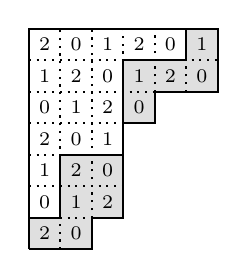
\begin{tikzpicture}[scale=0.4]
\draw[thick]  (0,0)--(2,0)--(2,1)--(3,1)--(3,4)--(4,4)--(4,5)--(6,5)--(6,7)--(0,7)--(0,0);
\draw[thick, fill=lightgray!50]  (0,0)--(2,0)--(2,1)--(3,1)--(3,3)--(1,3)--(1,1)--(0,1)--(0,0);
\draw[thick, fill=lightgray!50]  (0+3,4)--(1+3,4)--(1+3,5)--(3+3,5)--(3+3,7)--(2+3,7)--(2+3,6)--(0+3,6)--(0+3,4);
\draw[thick, dotted] (0,1)--(2,1);
\draw[thick, dotted] (0,2)--(3,2);
\draw[thick, dotted] (0,3)--(3,3);
\draw[thick, dotted] (0,4)--(3,4);
\draw[thick, dotted] (0,5)--(4,5);
\draw[thick, dotted] (0,6)--(6,6);
\draw[thick, dotted] (0,7)--(6,7);
\draw[thick, dotted] (0,0)--(0,7);
\draw[thick, dotted] (1,0)--(1,7);
\draw[thick, dotted] (2,1)--(2,7);
\draw[thick, dotted] (3,4)--(3,7);
\draw[thick, dotted] (4,5)--(4,7);
\draw[thick, dotted] (5,5)--(5,7);
\draw[thick, dotted] (6,6)--(6,7);
\node at (0.5,0.5){$\scriptstyle2 $};
\node at (0.5,1.5){$\scriptstyle0 $};
\node at (0.5,2.5){$\scriptstyle1 $};
\node at (0.5,3.5){$\scriptstyle 2 $};
\node at (0.5,4.5){$\scriptstyle0 $};
\node at (0.5,5.5){$\scriptstyle1 $};
\node at (0.5,6.5){$\scriptstyle2 $};
\node at (1.5,0.5){$\scriptstyle0 $};
\node at (1.5,1.5){$\scriptstyle1 $};
\node at (1.5,2.5){$\scriptstyle2 $};
\node at (1.5,3.5){$\scriptstyle 0 $};
\node at (1.5,4.5){$\scriptstyle1$};
\node at (1.5,5.5){$\scriptstyle2 $};
\node at (1.5,6.5){$\scriptstyle0 $};
\node at (2.5,1.5){$\scriptstyle2 $};
\node at (2.5,2.5){$\scriptstyle0 $};
\node at (2.5,3.5){$\scriptstyle 1 $};
\node at (2.5,4.5){$\scriptstyle2$};
\node at (2.5,5.5){$\scriptstyle0 $};
\node at (2.5,6.5){$\scriptstyle1 $};
\node at (3.5,4.5){$\scriptstyle0$};
\node at (3.5,5.5){$\scriptstyle1 $};
\node at (3.5,6.5){$\scriptstyle2 $};
\node at (4.5,5.5){$\scriptstyle2 $};
\node at (4.5,6.5){$\scriptstyle0 $};
\node at (5.5,5.5){$\scriptstyle0 $};
\node at (5.5,6.5){$\scriptstyle1 $};
\end{tikzpicture}
}
\;\;
\leftrightarrow
\;\;
\hackcenter{
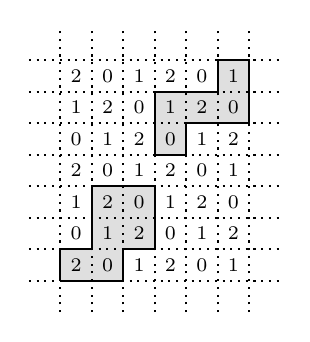
\begin{tikzpicture}[scale=0.4]
\draw[thick, fill=lightgray!50]  (0,0)--(2,0)--(2,1)--(3,1)--(3,3)--(1,3)--(1,1)--(0,1)--(0,0);
\draw[thick, fill=lightgray!50]  (0+3,4)--(1+3,4)--(1+3,5)--(3+3,5)--(3+3,7)--(2+3,7)--(2+3,6)--(0+3,6)--(0+3,4);
\draw[thick, dotted] (-1,0)--(7,0);
\draw[thick, dotted] (-1,1)--(7,1);
\draw[thick, dotted] (-1,2)--(7,2);
\draw[thick, dotted] (-1,3)--(7,3);
\draw[thick, dotted] (-1,4)--(7,4);
\draw[thick, dotted] (-1,5)--(7,5);
\draw[thick, dotted] (-1,6)--(7,6);
\draw[thick, dotted] (-1,7)--(7,7);
\draw[thick, dotted] (0,-1)--(0,8);
\draw[thick, dotted] (1,-1)--(1,8);
\draw[thick, dotted] (2,-1)--(2,8);
\draw[thick, dotted] (3,-1)--(3,8);
\draw[thick, dotted] (4,-1)--(4,8);
\draw[thick, dotted] (5,-1)--(5,8);
\draw[thick, dotted] (6,-1)--(6,8);
\node at (0.5,0.5){$\scriptstyle2 $};
\node at (0.5,1.5){$\scriptstyle0 $};
\node at (0.5,2.5){$\scriptstyle1 $};
\node at (0.5,3.5){$\scriptstyle 2 $};
\node at (0.5,4.5){$\scriptstyle0 $};
\node at (0.5,5.5){$\scriptstyle1 $};
\node at (0.5,6.5){$\scriptstyle2 $};
\node at (1.5,0.5){$\scriptstyle0 $};
\node at (1.5,1.5){$\scriptstyle1 $};
\node at (1.5,2.5){$\scriptstyle2 $};
\node at (1.5,3.5){$\scriptstyle 0 $};
\node at (1.5,4.5){$\scriptstyle1$};
\node at (1.5,5.5){$\scriptstyle2 $};
\node at (1.5,6.5){$\scriptstyle0 $};
\node at (2.5,0.5){$\scriptstyle1 $};
\node at (2.5,1.5){$\scriptstyle2 $};
\node at (2.5,2.5){$\scriptstyle0 $};
\node at (2.5,3.5){$\scriptstyle 1 $};
\node at (2.5,4.5){$\scriptstyle2$};
\node at (2.5,5.5){$\scriptstyle0 $};
\node at (2.5,6.5){$\scriptstyle1 $};
\node at (3.5,0.5){$\scriptstyle2 $};
\node at (3.5,1.5){$\scriptstyle0 $};
\node at (3.5,2.5){$\scriptstyle1 $};
\node at (3.5,3.5){$\scriptstyle 2 $};
\node at (3.5,4.5){$\scriptstyle0$};
\node at (3.5,5.5){$\scriptstyle1 $};
\node at (3.5,6.5){$\scriptstyle2 $};
\node at (4.5,0.5){$\scriptstyle0 $};
\node at (4.5,1.5){$\scriptstyle1 $};
\node at (4.5,2.5){$\scriptstyle2 $};
\node at (4.5,3.5){$\scriptstyle 0 $};
\node at (4.5,4.5){$\scriptstyle1$};
\node at (4.5,5.5){$\scriptstyle2 $};
\node at (4.5,6.5){$\scriptstyle0 $};
\node at (5.5,0.5){$\scriptstyle1 $};
\node at (5.5,1.5){$\scriptstyle2 $};
\node at (5.5,2.5){$\scriptstyle0 $};
\node at (5.5,3.5){$\scriptstyle 1 $};
\node at (5.5,4.5){$\scriptstyle2$};
\node at (5.5,5.5){$\scriptstyle0 $};
\node at (5.5,6.5){$\scriptstyle1 $};
\end{tikzpicture}
}
\;\;
\leftrightarrow
\;\;
\hackcenter{
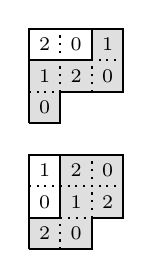
\begin{tikzpicture}[scale=0.4]
\draw[thick, fill=lightgray!50]  (0,0)--(2,0)--(2,1)--(3,1)--(3,3)--(1,3)--(1,1)--(0,1)--(0,0);
\draw[thick, fill=lightgray!50]  (0,4)--(1,4)--(1,5)--(3,5)--(3,7)--(2,7)--(2,6)--(0,6)--(0,4);
\draw[thick]  (0,1)--(1,1)--(1,3)--(0,3)--(0,1);
\draw[thick]  (0,6)--(2,6)--(2,7)--(0,7)--(0,6);
\draw[thick, dotted] (1,1)--(2,1);
\draw[thick, dotted] (0,2)--(3,2);
\draw[thick, dotted] (0,3)--(3,3);
\draw[thick, dotted] (0,0)--(0,3);
\draw[thick, dotted] (1,0)--(1,1);
\draw[thick, dotted] (2,1)--(2,3);
\draw[thick, dotted] (0,5)--(1,5);
\draw[thick, dotted] (0,6)--(3,6);
\draw[thick, dotted] (0,7)--(3,7);
\draw[thick, dotted] (0,5)--(0,7);
\draw[thick, dotted] (1,5)--(1,7);
\draw[thick, dotted] (2,5)--(2,7);
\node at (0.5,0.5){$\scriptstyle2 $};
\node at (0.5,1.5){$\scriptstyle0 $};
\node at (0.5,2.5){$\scriptstyle1 $};
\node at (1.5,0.5){$\scriptstyle0 $};
\node at (1.5,1.5){$\scriptstyle1 $};
\node at (1.5,2.5){$\scriptstyle2 $};
\node at (2.5,1.5){$\scriptstyle2 $};
\node at (2.5,2.5){$\scriptstyle0 $};
\node at (0.5,4.5){$\scriptstyle0 $};
\node at (0.5,5.5){$\scriptstyle1 $};
\node at (0.5,6.5){$\scriptstyle2 $};
\node at (1.5,5.5){$\scriptstyle2 $};
\node at (1.5,6.5){$\scriptstyle0 $};
\node at (2.5,5.5){$\scriptstyle0 $};
\node at (2.5,6.5){$\scriptstyle1 $};
\end{tikzpicture}
}
\end{align*}
\caption{Skew Young diagram \(\lambda^\tau/\mu^\tau\) with charge \(2\); Skew shape~\(\tau\); Level two skew Young diagram \(\blam/\bmu\) with multicharge \((2,1)\); all are associated as in \S\ref{otherformsec}}
\label{fig:Muth1}       
\end{figure}


\subsection{Ribbons and roots}
The following lemma establishes that the content of a ribbon depends only on the positions of the southwest/northeast end nodes, and not on the nodes in between.
\begin{lemma}\label{hookcont}
If \(\xi\) is a ribbon, then \(\cont(\xi) = \alpha(\res(\xi_{\ssww}), \dist(\xi_{\ssww},\xi_{\nnee})+1)\).
\end{lemma}
\begin{proof}
There is a \(\no/\ea\) path \((z^i)_{i=1}^{|\xi|}\) such that \(\xi = \{z^i\}_{i=1}^{|\xi|}\) by Lemma~\ref{hookispath}. We have then that \(z^1 = \xi_{\ssww}\) and \(z^{|\xi|} = \xi_{\nnee}\). Then by Lemma~\ref{sizehook} we have that \(|\xi| = \dist(\xi_{\ssww}, \xi_{\nnee})+1\), and so
\begin{align*}
\cont(\xi) &= \sum_{i=1}^{|\xi|} \alpha_{\res(z^i)} =
\sum_{i=0}^{\dist(\xi_{\ssww}, \xi_{\nnee})} \alpha_{ \res(\xi_{\ssww}) + \overline{i}}
=
 \alpha(\res(\xi_{\ssww}), \dist(\xi_{\ssww},\xi_{\nnee})+1),
\end{align*}
as desired.
\end{proof}



\begin{coro}\label{skewpos}
Let \(\beta \in Q_+\). Then \(\beta \in \Phi_+\) if and only if \(\beta = \cont(\xi)\) for some ribbon \(\xi\).
\end{coro}
\begin{proof}
We have by Lemma~\ref{hookcont} that \(\cont(\xi) \in \Phi_+\) for all ribbons \(\xi\). Now let \(\beta = \alpha(t,h) \in \Phi_+\). Let \(z \in \N_t\), and define nodes \(z^i = (z_1, z_2 + i-1)\) for \(i \in [1,h]\). Then \((z^i)_{i=1}^h\) is a \(\no/\ea\) path, and so \(\xi = \{z^i\}_{i=1}^h\) is a ribbon by Lemma~\ref{hookispath}. By construction, \(\xi_{\ssww} = z\), \(\xi_{\nnee} = (z_1, z_2+h-1)\), so \(\dist(\xi_{\ssww}, \xi_{\nnee}) = h-1\). Then by Lemma~\ref{hookcont} we have
\(
\cont(\xi) = \alpha(\res(z), h) = \alpha(t,h) = \beta,
\)
as desired.
\end{proof}

\section{Cuspidality}
Recall that we have fixed a convex preorder \(\succeq\) on \(\Phi_+\).
\begin{defi}\label{cuspdef}
Let \(\tau \in \SSSS(\beta)\) for some \(\beta \in \Phi_+\). We say that \(\tau\) is {\em cuspidal} provided that, for every tableau \((\lambda_1, \lambda_2)\) of \(\tau\), the following conditions hold:
\begin{enumerate}
\item There exist \(\gamma_1, \ldots, \gamma_k \in \Phi_+\) such that \(\cont(\lambda_1) = \gamma_1 + \cdots + \gamma_k\) and \(\beta \succ \gamma_i\) for all \(i \in [1,k]\), and; \label{cond:cuspdef1}
\item There exist \(\nu_1, \ldots, \nu_\ell \in \Phi_+\) such that \(\cont(\lambda_2) = \nu_1 + \cdots + \nu_\ell\) and \(\nu_i \succ \beta\) for all \(i \in [1,\ell]\). \label{cond:cuspdef2}
\end{enumerate}
\end{defi}

\begin{defi}\label{semicuspdef}
Let \( \tau \in \SSSS(m \beta)\) for some \(m \in \NN\), \(\beta \in \Phi_+\). We say that \(\tau\) is {\em semicuspidal} provided that, for every tableau \((\lambda_1, \lambda_2)\) of \(\tau\), the following conditions hold:
\begin{enumerate}
\item There exist \(\gamma_1, \ldots, \gamma_k \in \Phi_+\) such that \(\cont(\lambda_1) = \gamma_1 + \cdots + \gamma_k\) and \(\beta \succeq \gamma_i\) for all \(i \in [1,k]\), and;
\item There exist \(\nu_1, \ldots, \nu_\ell \in \Phi_+\) such that \(\cont(\lambda_2) = \nu_1 + \cdots + \nu_\ell\) and \(\nu_i \succeq \beta\) for all \(i \in [1,\ell]\).
\end{enumerate}
\end{defi}

It follows from definitions that cuspidality is invariant under \(e\)-similarity: 
\begin{lemma}
Let \(\tau, \nu\) be skew shapes, with \(\tau \sim_e \nu\). Then \(\tau\) is cuspidal (resp. semicuspidal) if and only if \(\nu\) is cuspidal (resp. semicuspidal). 
\end{lemma}


\begin{lemma}\label{shapehooktest}
If \(\tau\) is a cuspidal (resp. semicuspidal) skew shape, then for every \(\ssee\)-removable ribbon \(\xi \subsetneq \tau\) we have \(\cont(\xi) \succ \cont(\tau)\) (resp. \(\cont(\xi) \succeq \cont(\tau)\)).
\end{lemma}
\begin{proof}
 Let \(\tau\) be cuspidal. If \(\xi\) is an \(\ssee\)-removable ribbon in \(\tau\), then \((\tau \backslash \xi, \xi)\) is a skew decomposition for \(\tau\). 
 Then by the cuspidality property, we have \(\cont(\xi) = \gamma_1 + \cdots + \gamma_k\), for some positive roots \(\gamma_1, \ldots, \gamma_k \succ \cont(\tau)\). Then it follows by Corollary~\ref{skewpos} and Lemma~\ref{GenConvexLem}\eqref{cond:genconvex3} that \(\cont(\xi) \succ \cont(\tau)\). The proof in the semicuspidal case is similar.
\end{proof}


 \begin{lemma}\label{CuspForSkewHook}
Let \(\xi\) be a ribbon. Then \(\xi\) is cuspidal if and only if for every \(\ssee\)-removable ribbon \(\nu \subsetneq \xi\), we have \(\cont(\nu) \succ \cont(\xi)\).
 \end{lemma}
 \begin{proof}
The `only if' direction is provided by Lemma~\ref{shapehooktest}, so we focus on the `if' direction. 
 Assume that \(\xi\) is a ribbon with
 the property that \(\cont(\nu) \succ \cont(\xi)\) for every \(\ssee\)-removable ribbon \(\nu\) in \( \xi\). We have that \(\cont(\xi) \in \Phi_+\) by Corollary~\ref{skewpos}. We will show that \(\xi\) is cuspidal. 
 
 
 Let \((\varepsilon, \mu)\) be any tableau of \(\xi\). Let \(\mu_1, \ldots, \mu_t\) be the connected components of \(\mu\). Since each \(\mu_i\) is connected and a subset of a ribbon, and \((\varepsilon, \mu)\) is a tableau, we have that each \(\mu_i\) is an \(\ssee\)-removable ribbon in \(\xi\). Thus, by assumption, \(\cont(\mu_i) \succ \cont(\xi)\) for all \(i\). But then \(\cont(\mu) = \sum_{i=1}^t \cont(\mu_i)\), and so \(\xi\) satisfies condition \eqref{cond:cuspdef2} in Definition~\ref{cuspdef}.
 
 Let \(\varepsilon_1, \ldots, \varepsilon_u\) be the connected components of \(\varepsilon\). Again, each \(\varepsilon_i\) is a ribbon. Assume by way of contradiction there is some \(i\) such that \(\cont(\varepsilon_i) \succeq \cont(\xi)\). Since \((\varepsilon, \mu)\) is a tableau, we have that \((\varepsilon_i, \xi\backslash \varepsilon_i)\) is a tableau. By the previous paragraph, we have that \(\cont(\xi \backslash \varepsilon_i)\) can be written as a sum of positive roots \(\gamma_1 + \cdots + \gamma_s\), where \(\gamma_j \succ \cont(\xi)\) for all \(j \in [1,s]\). 
 If \(\cont(\varepsilon_i) \approx \cont(\xi)\), then we have that \(\cont(\varepsilon_i),\cont(\xi) \in \Phi_+^\im\) by Lemma~\ref{notapprox}. But this implies that \(\cont(\xi \backslash \varepsilon_i) = \cont(\xi) - \cont(\varepsilon_i) \in \Phi_+^\im\), and so \(\cont(\xi\backslash \varepsilon_i) \approx \cont(\xi)\). But since \(\cont(\xi \backslash \varepsilon_i) \in \Phi_+\), we have by Lemma~\ref{GenConvexLem}\eqref{cond:genconvex3} that \(\cont(\xi \backslash \varepsilon_i) =  \gamma_1 + \cdots + \gamma_s \succ \cont(\xi)\), a contradiction. Therefore \(\cont(\varepsilon_i) \succ \cont(\xi)\). But then we have by Lemma~\ref{GenConvexLem}\eqref{cond:genconvex3} that 
 \begin{align*}
 \cont(\xi) = \cont(\xi \backslash \varepsilon_i) + \cont(\varepsilon_i) = \gamma_1 + \cdots + \gamma_s + \cont(\varepsilon_i) \succ \cont(\xi),
 \end{align*}
 another contradiction. Therefore \(\cont(\varepsilon_i) \prec \cont(\xi)\) for all \(i \in [1,u]\). Since \(\cont(\varepsilon) = \sum_{i=1}^u \cont(\varepsilon_i)\), we have that \(\xi\) satisfies condition \eqref{cond:cuspdef1} in Definition~\ref{cuspdef}. Thus \(\xi\) is cuspidal.
 \end{proof}

 
 \subsection{Constructing cuspidal ribbons}\label{cuspcons}
For \(\beta \in \Psi\), we write \(\init(\beta) \subseteq \N\) for the set of nodes \(b \in \N\) such that \(\beta = \alpha(\res(b), \height(\beta))\). Note then that \(\init(\delta) = \N\), and if \(\beta \in \Phi_+^\re\) then \(\init(\beta) = \N_t\) for some \(t \in \Z_e\).
 

\begin{defi}\label{defxib}
Let \(\beta \in \Psi\) and \(b \in \init(\beta)\). Define a \(\no/\ea\) path \((z^i)_{i=1}^{\height(\beta)}\) by setting \(z^1 = b\), and 
\begin{align*}
z^i = \begin{cases}
\no z^{i-1} & \textup{if } \alpha(\res(b), i-1) \succ \beta;\\
\ea z^{i-1} & \textup{if } \beta \succ \alpha(\res(b), i-1),\\
\end{cases}
\end{align*}
for \(i = 2, \ldots, \height(\beta)\). Then define \(\zeta^{(\beta, b)} = \{z^i\}_{i=1}^{\height(\beta)}\).
\end{defi}

\begin{lemma}\label{zetaiscusp}
The set of nodes  
\(\zeta^{(\beta,b)}\) is a cuspidal ribbon of content \(\beta\), with \(\zeta^{(\beta,b)}_{\ssww} = b\).
\end{lemma}
\begin{proof}
First, note that the path \((z^i)_{i=1}^{\height(\beta)}\) is well-defined, which follows from Lemma~\ref{notapprox}\eqref{cond:notapprox2}. We have that \(\zeta^{(\beta,b)}\) is a ribbon by Lemma~\ref{hookispath}, and \(\cont(\zeta^{(\beta,b)}) = \beta\) by Lemma~\ref{hookcont}.

It remains to show that \( \zeta = \zeta^{(\beta,b)}\) is cuspidal. Let \(\nu \subsetneq \zeta\) be an \(\ssee\)-removable ribbon in \(\zeta\). By Lemma~\ref{CuspForSkewHook}, it will be enough to show that \(\cont(\nu) \succ \beta\). By Lemma~\ref{xiuv}, we have 
\(\nu = \xi^\zeta_{z^i,z^j}\) for some \(1 \leq i \leq j \leq h\), where \(\so z^i, \ea z^j \notin \zeta\). 


First assume \(i=1, j<h\). Since \(\ea z^j  \notin \zeta\), it follows from the construction of \(\zeta\) that \(z^{j+1} = \no z^j\), and thus \(\alpha(\res(b),j) \succ \beta\). But then by Lemma~\ref{hookcont} we have 
\begin{align*}
\cont(\nu) = \cont(\xi^\zeta_{z^1, z^j}) =  \alpha(\res(b),j) \succ \beta,
\end{align*}
as desired.

Now assume \(1<i\). Since \(\so z^i \notin \zeta\), we have \(z^i = \ea z^{i-1} \) and thus \(\beta \succ \alpha(\res(b), i-1)\). If \(j<h\), then since \(\ea z^j  \notin \zeta\), it follows from the construction of \(\zeta\) that \(z^{j+1} = \no z^j\), and thus \(\alpha(\res(b),j) \succ \beta\). On the other hand, if \(j=h\), then \(\alpha(\res(b),j) = \beta\), so in any case we have \(\alpha(\res(b),j) \succeq \beta\).
Therefore, applying Lemma~\ref{hookcont}, we have
\begin{align*}
\alpha(\res(b), j) &= 
\cont(\xi^\zeta_{z^1, z^j}) 
=\cont(\xi^\zeta_{z^1, z^{i-1}}\sqcup \xi^\zeta_{z^i, z^j})\\
&=
\cont(\xi^\zeta_{z^1, z^{i-1}}) + \cont(\xi^\zeta_{z^i, z^j})
= \alpha(\res(b), i-1) + \cont(\nu).
\end{align*}
If \(\beta \succeq \cont(\nu)\), we would have by Lemma~\ref{GenConvexLem}\eqref{cond:genconvex3} that \(\beta \succ \alpha(\res(b), j)\), a contradiction. Thus \(\cont(\nu) \succ \beta\), as desired.
\end{proof}


\begin{lemma}\label{onlycuspribbon}
Let \(\nu\) be a ribbon of content \(\beta \in \Psi\). Then \(\nu\) is cuspidal if and only if \(\nu = \zeta^{(\beta, \nu_{\ssww})}\).
\end{lemma}
\begin{proof}
The `if' direction is proved in Lemma~\ref{zetaiscusp}. Now we prove the `only if' direction. Let \(b =\nu_{\ssww}\), and \(h = \height(\beta)\). By Lemma~\ref{hookcont} we must have \(\beta = \alpha(\res(b),h)\). Consider the skew shape \(\zeta = \zeta^{(\beta,b)}\), and let \((z^i)_{i=1}^h\) be the \(\no/\ea\) path constructed in Definition~\ref{defxib} so that \(\zeta = \{z^i\}_{i=1}^h\). By Lemma~\ref{hookispath}, there is a \(\no/\ea\) path \((w^i)_{i=1}^h\), with \(w^1 = b\) and \(\nu = \{w^i\}_{i=1}^h\). Assume by way of contradiction that \(\nu \neq \zeta\). Then there exists \(2 \leq t \leq h\) such that \(w^i = z^i\) for \(i<t\), and \(w^t \neq z^t\). Note that by Lemma~\ref{notapprox}, we have \(\beta \not \approx \alpha(\res(b),t-1)\).

First assume \(\beta \succ \alpha(\res(b),t-1)\). Then \(z^t = \ea z^{t-1}\).
We have \(w^t \in \{\no w^{t-1}, \ea w^{t-1}\} = \{\no z^{t-1}, \ea z^{t-1}\}\), but \(w^t \neq z^t\), so \(w^t = \no z^{t-1}\). Then \(\ea w^{t-1} \notin \nu\), and \(\ea w^h \notin \nu\), so \(\xi^\nu_{w^1, w^{t-1}}\) is \(\ssee\)-removable in \(\nu\) by Lemma~\ref{xiuv}. By cuspidality of \(\nu\) and Lemma~\ref{CuspForSkewHook} we have that
\begin{align*}
\alpha(\res(\nu_1), t-1) \succ \cont(\xi^\nu_{\nu_t, \nu_h}) \succ \beta,
\end{align*}
a contradiction.

Now assume \(\alpha(\res(b),t-1) \succ \beta\). Then \(z^t = \no z^{t-1}\), and we have \(w^t \in \{\no w^{t-1}, \ea w^{t-1}\} = \{\no z^{t-1}, \ea z^{t-1}\}\), but \(w^t \neq z^t\), so \(w^t = \ea z^{t-1}\). Then \(\so w^t \notin \nu\), and \(\ea w^h \notin \nu\), so \(\xi^\nu_{w^t, w^h}\) is \(\ssee\)-removable in \(\nu\) by Lemma~\ref{xiuv}. By cuspidality of \(\nu\) and Lemma~\ref{CuspForSkewHook} we have that
\begin{align*}
\alpha(\res(w^t), h-t + 1) = \cont(\xi^\nu_{w^t, w^h}) \succ \beta.
\end{align*}
But then by convexity and (\ref{splithookcont}) we have
\begin{align*}
\beta = \alpha(\res(b), h) =  \alpha(\res(b),t-1) + \alpha(\res(w^t), h-t + 1) \succ \beta,
\end{align*}
a contradiction. Thus, in any case we derive a contradiction, so we must have \(\nu = \zeta\) as desired.
\end{proof}


\subsection{Distinguished cuspidal ribbons}
For each \(\beta \in \Phi_+^\re\), we make a distinguished choice of \(b^\beta \in \init(\beta)\). For each \(t \in \Z_e\), we make a distinguished choice of \(b^t \in \N_t\). Then we define the distinguished cuspidal ribbons, for all \(\beta \in \Phi_+^\re\) and \(t \in \N_t\):
\begin{align*}
\zeta^\beta := \zeta^{(\beta, b^{\beta})}, \qquad \zeta^t := \zeta^{(\delta, b^t)}
\end{align*}

By construction, the path associated with \(\zeta^{(\beta, b)}\) in Definition~\ref{defxib} relies only on \(\res(b)\) and \(\beta\), and not on the specific location of \(b\). Thus by Lemmas~\ref{zetaiscusp} and~\ref{onlycuspribbon} we have the following result:

\begin{prop}\label{allcusprib}
For all \(\beta \in \Phi_+^\re\), \(t \in \ZZ_e\), we have
\begin{align*}
[\zeta^{\beta}] = \{\zeta^{(\beta,b)} \mid b \in \init(\beta)\},
\qquad
\textup{and}
\qquad
[\zeta^{t}] = \{\zeta^{(\delta,b)} \mid b \in \N_t\}.
\end{align*}
The set \(\{\zeta^{\beta} \mid \beta \in \Phi_+^\re\} \cup \{\zeta^t \mid t \in \Z_e\}\) represents a complete and irredundant set of cuspidal ribbons with content in \(\Psi\), up to \(e\)-similarity.
\end{prop}

We will show in Theorem~\ref{allcusp} that this in fact describes all cuspidal {\em skew shapes} up to \(e\)-similarity.



\begin{exam}\label{e2shapes}
Take the case \(e=2\) and the convex preorder as defined in Example~\ref{e2order}. In this case we have a highly regular stairstep pattern for all real cuspidal ribbons, and a pair of two-node dominoes for the imaginary cuspidal ribbons, see Figure~\ref{fig:e2cusps}.
\begin{figure}
\begin{align*}
{}
\hackcenter{
\begin{tikzpicture}[scale=0.4]
\fill[fill=lightgray!50] (0,0)--(1,0)--(1,1)--(2,1)--(2,2)--(3,2)--(3,3)--(4,3)--(4,4)--(5,4)--(5,5)--(6,5)--(6,6)--(4,6)--(4,5)--(3,5)--(3,4)--(2,4)--(2,3)--(1,3)--(1,2)--(0,2)--(0,0);
\draw[thick] (4,3.5)--(4,4)--(5,4)--(5,5)--(6,5)--(6,6)--(4,6)--(4,5)--(3,5)--(3,4.5);
\draw[thick]  (1.5,3)--(1,3)--(1,2)--(0,2)--(0,0)--(1,0)--(1,1)--(2,1)--(2,2)--(2.5,2);
\draw[thick, dotted] (1,0)--(1,2);
\draw[thick, dotted] (2,1)--(2,3);
\draw[thick, dotted] (0,1)--(1,1);
\draw[thick, dotted] (1,2)--(2,2);
\draw[thick, dotted] (3,4)--(4,4)--(4,5)--(5,5)--(5,6);
\node at (0.5,0.5){$\scriptstyle1 $};
\node at (0.5,1.5){$\scriptstyle0 $};
\node at (1.5,1.5){$\scriptstyle1 $};
\node at (1.5,2.5){$\scriptstyle0 $};
\node at (3.5,4.5){$\scriptstyle0 $};
\node at (4.5,4.5){$\scriptstyle1 $};
\node at (4.5,5.5){$\scriptstyle0 $};
\node at (5.5,5.5){$\scriptstyle1 $};
\node at (2.75,3.5){$\scriptstyle \iddots $};
\end{tikzpicture}
}
\hackcenter{
\begin{tikzpicture}[scale=0.4]
\fill[fill=lightgray!50] (0,0)--(2,0)--(2,1)--(3,1)--(3,2)--(4,2)--(4,3)--(5,3)--(5,4)--(6,4)--(6,6)--(5,6)--(5,5)--(4,5)--(4,4)--(3,4)--(3,3)--(2,3)--(2,2)--(1,2)--(1,1)--(0,1)--(0,0);
\draw[thick] (4.5,3)--(5,3)--(5,4)--(6,4)--(6,6)--(5,6)--(5,5)--(4,5)--(4,4)--(3.5,4);
\draw[thick]  (2,2.5)--(2,2)--(1,2)--(1,1)--(0,1)--(0,0)--(2,0)--(2,1)--(3,1)--(3,1.5);
\draw[thick, dotted] (1,0)--(1,1)--(2,1)--(2,2)--(3,2);
\draw[thick, dotted] (4,3)--(4,4)--(5,4)--(5,5)--(6,5);
\node at (0.5,0.5){$\scriptstyle0 $};
\node at (1.5,0.5){$\scriptstyle1 $};
\node at (1.5,1.5){$\scriptstyle0 $};
\node at (2.5,1.5){$\scriptstyle1 $};
\node at (4.5,3.5){$\scriptstyle1 $};
\node at (4.5,4.5){$\scriptstyle0 $};
\node at (5.5,4.5){$\scriptstyle1 $};
\node at (5.5,5.5){$\scriptstyle0 $};
\node at (3.25,3){$\scriptstyle \iddots $};
\end{tikzpicture}
}
\qquad
\hackcenter{
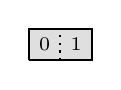
\begin{tikzpicture}[scale=0.4]
\fill[fill=lightgray!50] (0,0)--(2,0)--(2,1)--(0,1)--(0,0);
\draw[thick]  (0,0)--(2,0)--(2,1)--(0,1)--(0,0);
\draw[thick, dotted] (1,0)--(1,1);
\node at (0.5,0.5){$\scriptstyle0 $};
\node at (1.5,0.5){$\scriptstyle1 $};
\end{tikzpicture}
}
\qquad
\hackcenter{
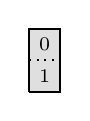
\begin{tikzpicture}[scale=0.4]
\fill[fill=lightgray!50] (0,0)--(1,0)--(1,2)--(0,2)--(0,0);
\draw[thick]  (0,0)--(1,0)--(1,2)--(0,2)--(0,0);
\draw[thick, dotted] (0,1)--(1,1);
\node at (0.5,0.5){$\scriptstyle1 $};
\node at (0.5,1.5){$\scriptstyle0 $};
\end{tikzpicture}
}
\end{align*}
\caption{Cuspidal ribbons, \(e=2\) case: \( \zeta^{n\delta + \alpha_1}; \zeta^{n \delta + \alpha_0}; \zeta^{ \overline{0}}; \zeta^{\overline{1}}\)}
\label{fig:e2cusps}      
\end{figure}
\end{exam}

We refer the reader to Example~\ref{BigEx} for a preorder in the \(e=3\) case with more irregular cuspidal ribbon shapes.


\subsection{Minimal ribbons}
Let \(\tau\) be a skew shape, and \(\xi\) be an \(\ssee\)-removable ribbon in \(\tau\). We say \(\xi\) is a {\em minimal \(\ssee\)-removable ribbon} (resp. {\em maximal}) provided that for every \(\ssee\)-removable ribbon \(\nu\) in \(\tau\) we have \(\cont(\nu) \succeq \cont(\xi)\) (resp. \(\cont(\nu) \preceq \cont(\xi)\)). We extend these notions as well to \(\nnww\)-removable ribbons in the obvious way.

\begin{lemma}\label{minremiscusp}
Let \(\xi\) be a minimal \(\ssee\)-removable ribbon in a skew shape \(\tau\), with \(\cont(\xi) \in \Psi\). Then \(\xi\) is cuspidal.
\end{lemma}
\begin{proof}
Take any \(\ssee\)-removable ribbon \(\nu \subsetneq \xi\) in \(\xi\). Since \(\xi\) is \(\ssee\)-removable in \(\tau\), we have that \(\nu\) is \(\ssee\)-removable in \(\tau\). By the minimality of \(\xi\), we have \(\cont(\nu) \succeq \cont(\xi)\), and by Lemma~\ref{notapprox}\eqref{cond:notapprox2} we have \(\cont(\nu) \not \approx \cont(\xi)\), so \(\cont(\nu) \succ \cont(\xi)\). Thus \(\xi\) is cuspidal by Lemma~\ref{CuspForSkewHook}.
\end{proof}

\begin{lemma}\label{mdeltaribbon}
If \(\nu\) is a ribbon of content \(m\delta\), then \(\nu\) has an \(\ssee\)-removable ribbon of content \(\delta\).
\end{lemma}
\begin{proof}
We go by induction on \(m\). The base case \(m=1\) is trivial, so assume \(m>1\) and make the induction assumption on \(m' < m\). By Lemma~\ref{hookispath} there exists a \(\no/\ea\) path \((z^i)_{i=1}^{me}\) such that \(\nu = \{z^i\}_{i=1}^{me}\). If \(z^{e+1} = \no z^e\), it follows by Lemma~\ref{xiuv} that \(\xi^\nu_{z^1, z^e}\) is \(\ssee\)-removable in \(\nu\), and we have \(\cont(\xi^\nu_{z^1,z^e}) = \delta\) by Lemma~\ref{hookcont}. On the other hand, if \(z^{e+1} = \ea z^e\), it follows by Lemma~\ref{xiuv} that \(\xi^\nu_{z^{e+1}, z^{me}}\) is \(\ssee\)-removable in \(\nu\), and we have \(\cont(\xi^\nu_{z^{e+1}, z^{me}}) = (m-1)\delta\) by Lemma~\ref{hookcont}. Then by induction there exists an \(\ssee\)-removable ribbon \(\omega\) in \(\xi^\nu_{z^{e+1}, z^{me}}\) of content \(\delta\). As \(\omega\) is \(\ssee\)-removable in \(\xi^\nu_{z^{e+1}, z^{me}}\), it is \(\ssee\)-removable in \(\nu\). This completes the induction step, and the proof.
\end{proof}


\begin{lemma}\label{minremexist}
If \(\tau\) is a skew shape, then \(\tau\) has a minimal \(\ssee\)-removable ribbon \(\xi\) such that \(\cont(\xi) \in \Psi\).
\end{lemma}
\begin{proof}
Let \(\nu\) be a minimal \(\ssee\)-removable ribbon in \(\tau\). Then \(\cont(\nu) \in \Phi_+\) by Lemma~\ref{hookcont}. If \(\cont(\nu) \in \Phi_+^\re\), we are done by (\ref{PsiDef}), so assume otherwise. Then 
by (\ref{allimag}), we have \(\cont(\nu) = m\delta\) for some \(m\in \NN\).
Then by Lemma~\ref{mdeltaribbon}, \(\nu\) has an \(\ssee\)-removable ribbon \(\xi\) of content \(\delta \in \Psi\). But then \(\xi\) is \(\ssee\)-removable in \(\tau\), and \(\delta \approx m\delta\), so \(\xi\) is minimal in \(\tau\) as well.
\end{proof}

The next key lemma establishes that consecutively \(\ssee\)-removed minimal ribbons are non-decreasing in the convex preorder. 

 \begin{lemma}\label{remsinorder}
Let \(\tau\) be a skew shape. Let \(\xi_1\) be a minimal \(\ssee\)-removable ribbon in \(\tau\), and let \(\xi_2\) be a minimal \(\ssee\)-removable ribbon in \(\tau'=\tau\backslash \xi_1\). Then \(\cont(\xi_2) \succeq \cont(\xi_1)\).
 \end{lemma}
 \begin{proof}
First, note that if \(\xi_1 \sqcup \xi_2\) is disconnected, then \(\xi_2\) is an \(\ssee\)-removable ribbon in \(\tau\), so by minimality of \(\xi_1\), we would have \(\cont(\xi_2) \succeq \cont(\xi_1)\), as desired. Thus we may assume \(\xi_1 \sqcup \xi_2\) is a connected skew shape, and therefore \(\xi_1, \xi_2\) belong to the same connected component of \(\tau\). 
  We have \(\xi_1 = \xi^\tau_{u,v}\) for some \((u,v) \in \textup{Rem}_\tau\), and \(\xi_2 = \xi^{\tau'}_{z,w}\) for some \((z,w) \in \textup{Rem}_{\tau'}\), where \(u,v,z,w\) belong to the same connected component of \(\tau\).  
We consider the six possible cases of arrangements of the nodes \(u,v,z,w\) separately.
 
 {\em Case 1: Assume \(u \nearrow v \nearrow z \nearrow w\).} First, note that since \(\xi_1 \sqcup \xi_2\) is connected, we must have \(z \in \{\no v, \ea v\}\). But, since \((u,v) \in \textup{Rem}_\tau\), we have \(\ea v \notin \tau\), so \(z=\no v\). 
By Lemma~\ref{remhookswap}\eqref{cond:remhookswap1} we have that \((u,w) \in \textup{Rem}_\tau\) and \(\xi^\tau_{u,w}\) is an \(\ssee\)-removable ribbon in \(\tau\) by Lemma~\ref{xiuv}.
 
We have
\begin{align*}
\dist(u,w) = 
\dist(u,v) + \dist(v,z) + \dist(z,w) = 
 \dist(u,v) + \dist(z,w) + 1
\end{align*}
and
\begin{align*}
\res(z) = \res(\ea v) = \res(v) + \overline{1} = \res(u) + \overline{\dist(u,v) + 1}.
\end{align*}
It follows by (\ref{splithookcont}) and Lemma~\ref{hookcont} that 
\begin{align*}
\cont(\xi^\tau_{u,w}) &= \alpha(\res(u), \dist(u,w)+1) = \alpha(\res(u),  \dist(u,v) + \dist(z,w) + 2)\\
&= \alpha(\res(u), \dist(u,v)+1) + \alpha(\res(u) + \overline{\dist(u,v)+1}, \dist(z,w)+1)\\
&= \alpha(\res(u),  \dist(u,v)+1) + \alpha(\res(z), \dist(z,w)+1)\\
&= \cont(\xi_1) + \cont(\xi_2).
\end{align*}

Assume by way of contradiction that \(\cont(\xi_1) \succ \cont(\xi_2)\). Then we have \(\cont(\xi_1) \succ \cont(\xi^\tau_{u,w}) \succ \cont(\xi_2)\) by Lemma~\ref{GenConvexLem}. But, since \(\xi^\tau_{u,w}\) is \(\ssee\)-removable in \(\tau\), this contradicts \(\xi_1\) being a minimal \(\ssee\)-removable ribbon in \(\tau\). Therefore \(\cont(\xi_2) \succeq \cont(\xi_1)\), as desired.

 {\em Case 2: Assume \(w \nearrow u\).} Note that since \(\xi_1 \sqcup \xi_2\) is connected, we must have \(w \in \{\so u, \we u\}\). But, since \((u,v) \in \textup{Rem}_\tau\),
we have \(\so u \notin \tau\), so \(w=\we u\). We have by Lemma~\ref{remhookswap}\eqref{cond:remhookswap2} that \((z,v) \in \textup{Rem}_\tau\). Therefore \(\xi^\tau_{z,v}\) is an \(\ssee\)-removable ribbon in \(\tau\) by Lemma~\ref{xiuv}. 
 It can be shown along the lines of Case 1 that \(\cont(\xi^\tau_{z,v}) = \cont(\xi_1) + \cont(\xi_2)\). Thus if \(\cont(\xi_1) \succ \cont(\xi_2)\), we derive a contradiction along the same lines as Case 1 as well, so we have \(\cont(\xi_2) \succeq \cont(\xi_1)\), as desired.
 
 {\em Case 3: Assume \(u \nearrow z \nearrow v \nearrow w\)}. It follows from Lemma~\ref{remhookswap}\eqref{cond:remhookswap3} that \((\ssee z, w) \in \textup{Rem}_\tau\). 
Therefore \(\xi^\tau_{\ssee z,w}\) is an \(\ssee\)-removable ribbon in \(\tau\) by Lemma~\ref{xiuv}.
 We have
\(
 \dist(\ssee z ,w) = \dist(z,w),
\)
 and
\(
 \res(\ssee z) =\res(z),
\)
 so by Lemma~\ref{hookcont} it follows that 
 \begin{align*}
 \cont(\xi^\tau_{\ssee z,w}) &= \alpha(\res(\ssee z), \dist(\ssee z,w)+1)\\
 &= \alpha(\res(z),\dist(z,w)+1) = \cont(\xi_2).
 \end{align*}
As \(\xi_1\) is a minimal \(\ssee\)-removable ribbon in \(\tau\), we have then that
\(
\cont(\xi_2) = \cont(\xi^\tau_{\ssee z,w}) \succeq \cont(\xi_1),
\)
as desired.

{\em Case 4: Assume \(z \nearrow u \nearrow w \nearrow v\)}. 
It follows from Lemma~\ref{remhookswap}\eqref{cond:remhookswap4} that \((z, \ssee w) \in \textup{Rem}_\tau\).
Therefore \(\xi^\tau_{z, \ssee w}\) is an \(\ssee\)-removable ribbon in \(\tau\) by Lemma~\ref{xiuv}.
As in Case 3, it is straightforward to show that \(\cont(\xi^\tau_{z, \ssee w}) = \cont(\xi_2)\), and thus by the minimality of \(\xi_1\) we have
\(
\cont(\xi_2) = \cont(\xi^\tau_{z, \ssee w}) \succeq \cont(\xi_1),
\)
as desired.

{\em Case 5: Assume \(u \nearrow z \nearrow w \nearrow v\)}. It follows from Lemma~\ref{remhookswap}\eqref{cond:remhookswap5} that \((\ssee z, \ssee w) \in \textup{Rem}_\tau\tau\). Then \(\xi^\tau_{\ssee z, \ssee w}\) is an \(\ssee\)-removable ribbon in \(\tau\). 

We have
\(
 \dist(\ssee z,\ssee w) = \dist (z,w),
\)
 and
\(
 \res(\ssee z) = \res(z)
\), so it follows by Lemma~\ref{hookcont} that 
 \begin{align*}
 \cont(\xi^\tau_{\ssee z,\ssee w}) &= \alpha(\res(\ssee z), \dist(\ssee z,\ssee w)+1)\\
 &= \alpha(\res(z),\dist(z,w)+1) = \cont(\xi_2).
 \end{align*}
As \(\xi_1\) is a minimal \(\ssee\)-removable ribbon in \(\tau\), it follows that
\(
\cont(\xi_2) = \cont(\xi^\tau_{\ssee(z),w}) \succeq \cont(\xi_1),
\)
as desired.

{\em Case 6: Assume \(z \nearrow u \nearrow v \nearrow w\)}.  It follows from Lemma~\ref{remhookswap}\eqref{cond:remhookswap6} that \((z, w) \in \textup{Rem}_\tau\tau\). Thus \(\xi^\tau_{z,w}\) is an \(\ssee\)-removable ribbon in \(\tau\). 
But then by Lemma~\ref{xiuv} and the minimality of \(\xi_1\) we have
\(
\cont(\xi_2) =\cont(\xi^\tau_{z,w}) \succeq \cont(\xi_1),
\)
as desired, completing the proof. 
\end{proof}

\section{Kostant partitions and tilings}\label{Kostsec}



\subsection{Kostant partitions}
For \(\theta \in Q_+\), a {\em Kostant partition} of \(\gamma\) is a tuple of non-negative integers \(\bkap = (\kappa_\beta)_{\beta \in \Psi}\) such that \(\sum_{\beta \in \Psi} \kappa_\beta \beta = \theta\). If \(\beta_1 \succ \cdots \succ \beta_k\) are the members of \(\Psi\) such that \(\kappa_{\beta_1} \neq 0\), then it is convenient to write \(\bkap\) in the form
\begin{align*}
\bkap = 
(\beta_1^{\kappa_{\beta_1}} \mid \ldots \mid \beta_k^{\kappa_{\beta_k}}).
\end{align*}

We write \(\Xi(\theta)\) for the set of all Kostant partitions of \(\theta\).
The convex preorder \(\succeq\) on \(\Phi_+\) restricts to a total order \(\succ\) on \(\Psi\), which induces a right lexicographic total order \(\triangleright_R\) on \(\Xi(\beta)\), where
\begin{align*}
\bkap \triangleright_R \bkap'
\iff
\textup{there exists \(\beta \in \Psi\) such that }
\kappa_\beta > \kappa'_\beta \textup{ and } \kappa_\nu = \kappa'_\nu \textup{ for all } \beta \succ \nu.
\qquad
\end{align*}
We also have a 
left lexicographic total order \(\triangleright_L\) on \(\Xi(\beta)\), where
\begin{align*}
\bkap \triangleright_L \bkap'
\iff
\textup{there exists \(\beta \in \Psi\) such that }
\kappa_\beta > \kappa'_\beta \textup{ and } \kappa_\nu = \kappa'_\nu \textup{ for all } \beta \prec \nu.
\qquad
\end{align*}
Then the orders \(\triangleright_R\), \(\triangleright_L\) induce a bilexicographic partial order \(\trianglerighteq\) on \(\Xi(\beta)\), given by
\begin{align*}
\bkap \trianglerighteq \bkap'
\qquad
\iff
\qquad
\bkap \trianglerighteq_R \bkap'
\textup{ and }
\bkap \trianglerighteq_L \bkap'.
\end{align*}

For a sequence \(\bbeta = (\beta_i)_{i=1}^k\) of elements of \(\Phi_+'\), we say \(\bbeta\) is a {\em Kostant sequence} if \(\psi(\beta_i) \succeq \psi(\beta_j)\) whenever \(i \leq j\).
To any Kostant sequence \(\bbeta = (\beta_i)_{i=1}^k\) we may associate a Kostant partition \(\bkap^{\bbeta}\) by setting
\begin{align*}
\kappa^{\bbeta}_\nu = \sum_{ i\in [1,k], \psi(\beta_i) = \nu} m(\beta_i) \qquad \qquad(\nu \in \Psi).
\end{align*}


\subsection{Kostant tilings}
We say a tiling \(\Lambda\) of a skew shape \(\tau\) is a {\em ribbon} (resp. {\em cuspidal}, {\em semicuspidal}) tiling if \(\lambda\) is a ribbon (resp. cuspidal skew shape, semicuspidal skew shape) for all \(\lambda \in \Lambda\).
We are particularly interested in such tilings whose constituent skew shapes are arranged in a way that respects the convex preorder \(\succeq\), as follows.

\begin{defi}
Assume that \(\Lambda\) is a tiling of a skew shape \(\tau\) such that \(\cont(\lambda) \in \Phi_+'\) for all \(\lambda\in \Lambda\), and there exists a \(\Lambda\)-tableau \(\ttt\) such that \((\cont(\ttt(i)))_{i=1}^{|\Lambda|}\) is a Kostant sequence. Then we say \(\Lambda\) is a {\em Kostant} tiling, and that \((\Lambda,\ttt)\) is a {\em Kostant} tableau for~\(\tau\).
\end{defi}

If \((\Lambda,\ttt)\) is a Kostant tableau for \(\tau\), then we have an associated Kostant sequence \(\bbeta^{\ttt}:= (\cont(\ttt(i)))_{i=1}^{|\Lambda|}\), and associated Kostant partition \(\bkap^\Lambda = \bkap^{\bbeta^{\ttt}}\). The Kostant partition \(\bkap^\Lambda\) depends only on \(\Lambda\) and not on the choice of \(\Lambda\)-tableau \(\ttt\).

\begin{defi}
Let \(\tau\) be a skew shape, and let \((\Lambda,\ttt)\) be a tableau for \(\tau\). 
We say \((\Lambda,\ttt)\) is a {\em minimal \(\ssee\)-removable ribbon tableau} of \(\tau\) provided that \(\cont(\lambda_j) \in \Psi\) and \(\lambda_j\) is a minimal \(\ssee\)-removable ribbon in \(\bigsqcup_{i=1}^j \lambda_i\) for all \(j \in [1, |\Lambda|]\). We say \(\Lambda\) is a {\em minimal \(\ssee\)-removable ribbon tiling} of \(\tau\) if there exists a \(\Lambda\)-tableau \(\ttt\) such that \((\Lambda, \ttt)\) is a minimal \(\ssee\)-removable ribbon tableau.
\end{defi}

We have the following dual notion as well:

\begin{defi}
Let \(\tau\) be a skew shape, and let \((\Lambda,\ttt)\) be a tableau for \(\tau\). 
We say \((\Lambda,\ttt)\) is a {\em maximal \(\nnww\)-removable ribbon tableau} of \(\tau\) provided that \(\cont(\lambda_j) \in \Psi\) and \(\lambda_j\) is a maximal \(\nnww\)-removable ribbon in \(\bigsqcup_{i=j}^{|\Lambda|} \lambda_i\) for all \(j \in [1, |\Lambda|]\). We say \(\Lambda\) is a {\em maximal \(\nnww\)-removable ribbon tiling} of \(\tau\) if there exists a \(\Lambda\)-tableau \(\ttt\) such that \((\Lambda, \ttt)\) is a maximal \(\nnww\)-removable ribbon tableau.
\end{defi}

\begin{exam}\label{e2Kosex}
Take \(e=2\) and recall the convex preorder \(\succeq\) from Example~\ref{e2order} and the cuspidal ribbons from Example~\ref{e2shapes}. We show two tilings for a skew shape \(\tau\) in Figure~\ref{fig:Kosex1}. The tiling \(\Lambda_1\) on the left is Kostant for this preorder, with associated Kostant partition
\begin{align*}
\bkap^{\Lambda_1} = ( 3\delta + \alpha_1 \mid  \delta^3 \mid \delta + \alpha_0).
\end{align*}
The tiling \(\Lambda_2\) on the right in Figure~\ref{fig:Kosex1} is a cuspidal Kostant tiling for \(\tau\), which is (not coincidentally, per Theorem~\ref{mainthmcusp}) a minimal \(\ssee\)-removable ribbon tiling, and maximal \(\nnww\)-removable ribbon tiling as well. The associated Kostant partition is
\begin{align*}
\bkap^{\Lambda_2} = (\alpha_1^2 \mid \delta + \alpha_1 \mid  \delta^3 \mid \delta + \alpha_0 \mid \alpha_0^2).
\end{align*}
\end{exam}



\begin{figure}
\begin{align*}
{}
\hackcenter{
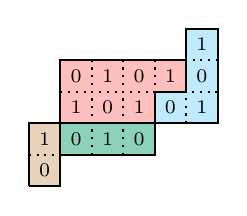
\begin{tikzpicture}[scale=0.4]
\draw[thick, fill=brown!35]  (0,-1)--(1,-1)--(1,0)--(4,0)--(4,1)--(6,1)--(6,4)--(5,4)--(5,3)--(1,3)--(1,2)--(1,1)--(0,1)--(0,-1);
\draw[thick, fill=pink]  (1,1)--(4,1)--(4,2)--(5,2)--(5,3)--(1,3)--(1,1);
\draw[thick, fill=cyan!25]  (4,1)--(6,1)--(6,4)--(5,4)--(5,2)--(4,2)--(4,1);
\draw[thick,  fill=blue!40!green!45]  (1,0)--(4,0)--(4,1)--(1,1)--(1,0);
\draw[thick, dotted] (1,0)--(1,1);
\draw[thick, dotted] (2,0)--(2,3);
\draw[thick, dotted] (3,0)--(3,3);
\draw[thick, dotted] (4,0)--(4,3);
\draw[thick, dotted] (5,1)--(5,3);
\draw[thick, dotted] (0,0)--(4,0);
\draw[thick, dotted] (0,1)--(6,1);
\draw[thick, dotted] (1,2)--(6,2);
\draw[thick, dotted] (2,3)--(6,3);
\draw[thick]   (0,-1)--(1,-1)--(1,0)--(4,0)--(4,1)--(6,1)--(6,4)--(5,4)--(5,3)--(1,3)--(1,2)--(1,1)--(0,1)--(0,-1);
\node at (0.5,-0.5){$\scriptstyle0 $};
\node at (0.5,0.5){$\scriptstyle1 $};
\node at (1.5,0.5){$\scriptstyle0 $};
\node at (2.5,0.5){$\scriptstyle1 $};
\node at (3.5,0.5){$\scriptstyle0 $};
\node at (1.5,1.5){$\scriptstyle1 $};
\node at (2.5,1.5){$\scriptstyle0 $};
\node at (3.5,1.5){$\scriptstyle1 $};
\node at (4.5,1.5){$\scriptstyle0 $};
\node at (5.5,1.5){$\scriptstyle1 $};
\node at (1.5,2.5){$\scriptstyle0 $};
\node at (2.5,2.5){$\scriptstyle1 $};
\node at (3.5,2.5){$\scriptstyle0 $};
\node at (4.5,2.5){$\scriptstyle1 $};
\node at (5.5,2.5){$\scriptstyle0 $};
\node at (5.5,3.5){$\scriptstyle1 $};
\end{tikzpicture}
}
\qquad
\qquad
\hackcenter{
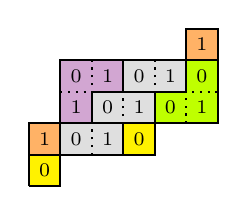
\begin{tikzpicture}[scale=0.4]
\draw[thick,  fill=violet!35]  (0,-1)--(1,-1)--(1,0)--(4,0)--(4,1)--(6,1)--(6,4)--(5,4)--(5,3)--(1,3)--(1,2)--(1,1)--(0,1)--(0,-1);
\draw[thick, fill=yellow]  (0,-1)--(1,-1)--(1,0)--(0,0)--(0,-1);
\draw[thick, fill=orange!60]  (0,0)--(1,0)--(1,1)--(0,1)--(0,0);
\draw[thick, fill=yellow]  (3,0)--(4,0)--(4,1)--(3,1)--(3,0);
\draw[thick, fill=lightgray!50]  (1,0)--(3,0)--(3,1)--(4,1)--(4,2)--(5,2)--(5,3)--(3,3)--(3,2)--(2,2)--(2,1)--(1,1)--(1,0);
\draw[thick]  (2,1)--(3,1);
\draw[thick]  (3,2)--(4,2);
\draw[thick, fill=lime] (4,1)--(6,1)--(6,3)--(5,3)--(5,2)--(4,2)--(4,1);
\draw[thick, fill=orange!60]  (5,3)--(6,3)--(6,4)--(5,4)--(5,3);
\draw[thick, dotted] (1,0)--(1,1);
\draw[thick, dotted] (2,0)--(2,3);
\draw[thick, dotted] (3,0)--(3,3);
\draw[thick, dotted] (4,0)--(4,3);
\draw[thick, dotted] (5,1)--(5,3);
\draw[thick, dotted] (0,0)--(4,0);
\draw[thick, dotted] (0,1)--(6,1);
\draw[thick, dotted] (1,2)--(6,2);
\draw[thick, dotted] (2,3)--(6,3);
\draw[thick]   (0,-1)--(1,-1)--(1,0)--(4,0)--(4,1)--(6,1)--(6,4)--(5,4)--(5,3)--(1,3)--(1,2)--(1,1)--(0,1)--(0,-1);
\node at (0.5,-0.5){$\scriptstyle0 $};
\node at (0.5,0.5){$\scriptstyle1 $};
\node at (1.5,0.5){$\scriptstyle0 $};
\node at (2.5,0.5){$\scriptstyle1 $};
\node at (3.5,0.5){$\scriptstyle0 $};
\node at (1.5,1.5){$\scriptstyle1 $};
\node at (2.5,1.5){$\scriptstyle0 $};
\node at (3.5,1.5){$\scriptstyle1 $};
\node at (4.5,1.5){$\scriptstyle0 $};
\node at (5.5,1.5){$\scriptstyle1 $};
\node at (1.5,2.5){$\scriptstyle0 $};
\node at (2.5,2.5){$\scriptstyle1 $};
\node at (3.5,2.5){$\scriptstyle0 $};
\node at (4.5,2.5){$\scriptstyle1 $};
\node at (5.5,2.5){$\scriptstyle0 $};
\node at (5.5,3.5){$\scriptstyle1 $};
\end{tikzpicture}
}
\end{align*}
\caption{Kostant tiling for \(\tau\); cuspidal Kostant tiling for \(\tau\)}
\label{fig:Kosex1}      
\end{figure}


\subsection{Results on Kostant tilings}\label{resKos}

\begin{lemma}\label{minremtab}
Every nonempty skew shape \(\tau\) has a minimal \(\ssee\)-removable ribbon tableau \((\Lambda,\ttt)\).
\end{lemma}
\begin{proof}
We go by induction on \(|\tau|\). If \(|\tau| = 1\), then we trivially take \(\Lambda = \{\tau\}\) and \(\ttt(1) = \tau\). Now let \(|\tau|>1\) and make the induction assumption on skew shapes \(\tau'\) with \(|\tau'| <|\tau|\).
By Lemma~\ref{minremexist}, \(\tau\) has a minimal \(\ssee\)-removable ribbon \(\xi\) such that \(\cont(\xi) \in \Psi\). Let \(\tau' = \tau \backslash \xi\). If \(\tau' = \varnothing\), we are done, taking \(\Lambda = \{\xi\}\), \(\ttt(1) = \xi\). Assume \(\tau' \neq \varnothing\). Then \(\tau'\) is a skew shape by Lemma~\ref{tabisskew}, which by the induction assumption has a minimal \(\ssee\)-removable ribbon tableau \((\Lambda', \ttt')\). But then taking \(\Lambda = \Lambda' \cup \{\xi\}\), \(\ttt(i) = \ttt'(i)\), \(\ttt(|\Lambda|) = \xi\), for all \(i \in [1,|\Lambda'|]\), we have that \((\Lambda, \ttt)\) is a minimal \(\ssee\)-removable ribbon tableau for \(\tau\).
\end{proof}

\begin{lemma}\label{minremtabisKos}
If \((\Lambda,\ttt)\) is a minimal \(\ssee\)-removable ribbon tableau for a skew shape \(\tau\), then \((\Lambda,\ttt)\) is a cuspidal Kostant tableau for \(\tau\).
\end{lemma}
\begin{proof}
By Lemma~\ref{minremiscusp}, every \(\lambda \in \Lambda\) is cuspidal, so it remains to verify that \((\cont(\ttt(i)))_{i=1}^{|\Lambda|}\) is a Kostant sequence by showing that \(\cont(\ttt(j)) \succeq \cont(\ttt(j+1))\) for all \(j \in [1,|\Lambda|-1]\). Indeed, \(\ttt(j+1)\) is a minimal \(\ssee\)-removable ribbon tableau in \(\bigsqcup_{i=1}^{j+1}\ttt(i)\), and \(\ttt(i)\) is a minimal \(\ssee\)-removable ribbon tableau in \(\bigsqcup_{i=1}^{j} \ttt(i)= (\bigsqcup_{i=1}^{j+1}\ttt(i)) \backslash \ttt(j+1)\), so the result follows by Lemma~\ref{remsinorder}.
\end{proof}

\begin{lemma}\label{cuspisribbon}
Every cuspidal skew shape is a ribbon.
\end{lemma}
\begin{proof}
Let \(\tau\) be a cuspidal skew shape, so that \(\cont(\tau) \in \Phi_+\), and assume by way of contradiction that \(\tau\) is not a ribbon. By Lemma~\ref{minremtab}, there exists a minimal \(\ssee\)-removable ribbon tableau for \(\tau\). As \(\tau\) is not itself a ribbon, it must be that \(|\Lambda|>1\). By Lemma~\ref{minremtabisKos} we have 
\begin{align*}
\cont(\ttt(1)) \succeq \cdots \succeq \cont(\ttt(|\Lambda|)).
\end{align*}
As
\(
\cont(\ttt(1)) + \cdots + \cont(\ttt(|\Lambda|)) = \cont(\tau), 
\)
we have by Lemma~\ref{GenConvexLem} that
\begin{align*}
\cont(\ttt(1)) \succeq \cont(\tau)\succeq \cont(\ttt(|\Lambda|)).
\end{align*}
But \(\ttt(|\Lambda|)\) is a minimal \(\ssee\)-removable ribbon in \(\tau\), so \(\cont(\ttt(|\Lambda|)) \succ \cont(\tau)\) by Lemma~\ref{shapehooktest}, giving the desired contradiction.
\end{proof}

\begin{lemma}\label{cuspisindiv}
If \(\xi\) is a cuspidal skew shape, then \(\cont(\xi) \in \Psi\).
\end{lemma}
\begin{proof}
By Lemma~\ref{cuspisribbon} we have that \(\xi\) is a ribbon. If \(\cont(\xi) \in \Phi_+ \backslash \Psi\), then \(\cont(\xi) = m\delta\) for some \(m >1\). But then \(\xi\) has an \(\ssee\)-removable skew hook \(\nu \subsetneq \xi\) of content \(\cont(\xi) \succeq \delta\), a contradiction of Lemma~\ref{CuspForSkewHook}, so \(\cont(\xi) \in \Psi\).
\end{proof}



\begin{lemma}\label{othersmaller}
Let \(\Lambda\) be a minimal \(\ssee\)-removable ribbon tiling for \(\tau\), and \(\Lambda'\) be a Kostant tiling for \(\tau\). Then \(\bkap^\Lambda \trianglerighteq_R \bkap^{\Lambda'}\), and \(\bkap^\Lambda = \bkap^{\Lambda'}\) if and only if every \(\lambda' \in \Lambda'\) is a union of tiles \(\lambda \in \Lambda\) with \(\psi(\cont(\lambda')) = \cont(\lambda)\).
\end{lemma}
\begin{proof}
For sake of space, if \(\Lambda, \Lambda'\) are such that every \(\lambda' \in \Lambda'\) is a union of tiles \(\lambda \in \Lambda\) with \(\psi(\cont(\lambda')) = \cont(\lambda)\), we will refer to this as the `union condition'. It is clear from the definition of \(\bkap^\Lambda\), \(\bkap^{\Lambda'}\) that \(\bkap^\Lambda = \bkap^{\Lambda'}\) when \(\Lambda, \Lambda'\) satisfy the union condition.

We prove the claim by induction on \(|\tau|\), the base case \(|\tau| = 1\) being trivial. Assume that \(|\tau| >1\), and the claim holds for all \(\tau'\) with \(|\tau'| < |\tau|\). There exists some \(\nu \in \Lambda'\) which is \(\ssee\)-removable in \(\tau\) and \(\psi(\cont(\nu')) \succeq \psi(\cont(\nu))\) for all \(\nu' \in \Lambda'\).

For all \(\lambda \in \Lambda\), set \(\nu^\lambda = \nu \cap \lambda\). Set \(\Lambda_0 = \{\lambda \in \Lambda \mid \nu^\lambda = \lambda\}\) and \(\Lambda_1 = \{\lambda \in \Lambda \mid \nu^\lambda \neq \varnothing, \lambda\}\).
By Lemma~\ref{minremtabisKos}, each \(\lambda \in \Lambda\) is cuspidal, and \(\nu^\lambda\) is \(\ssee\)-removable in each \(\lambda\) because \(\nu\) is \(\ssee\)-removable in \(\tau\). Thus, for all \(\lambda \in \Lambda_1\), we have
 \(
\cont(\nu^\lambda) = \beta^{\lambda, 1} + \cdots + \beta^{\lambda, r_\lambda}
\)
for some \(\cont(\lambda) \prec \beta^{\lambda, 1}, \cdots, \beta^{\lambda, r_\lambda} \in \Phi_+\). Then we have
\begin{align*}
\cont(\nu) = \sum_{\lambda \in \Lambda_0} \cont(\lambda) + \sum_{\Lambda \in \Lambda_1} \beta^{\lambda, 1} + \cdots + \beta^{\lambda, r_{\lambda}}.
\end{align*}

If there exists \(\lambda \in \Lambda_0\) such that \(\psi(\cont(\nu)) \succ \cont(\lambda)\), then \(\Lambda, \Lambda'\) do not satisfy the union condition, and we have \(\bkap^\Lambda \triangleright_R \bkap^{\Lambda'}\). If there exists \(\lambda \in \Lambda_1\), \(j \in [1, r_\lambda]\) such that \(\psi(\cont(\nu)) \succeq \beta^{\lambda, j}\), then \(\Lambda, \Lambda'\) do not satisfy the union condition, and we again have \(\psi(\cont(\nu)) \succ \cont(\lambda)\), so \(\bkap^\Lambda \triangleright_R \bkap^{\Lambda'}\). 

We may assume then that \(\cont(\lambda) \succeq \psi(\cont(\nu))\) for all \(\lambda \in \Lambda_0\) and \(\beta^{\lambda,j} \succ \psi(\cont(\nu))\) for all \(\lambda \in \Lambda_1, j \in [1,r_\lambda]\). By Lemma~\ref{GenConvexLem}, this implies that \(\Lambda_1 = \varnothing\), and \(\cont(\lambda) = \psi(\cont(\nu))\) for all \(\lambda \in \Lambda_0\). If \(\tau':=\tau \backslash \nu = \varnothing\), then we are done, as \(\Lambda, \Lambda'\) satisfy the union condition and \(\bkap^\Lambda = \bkap^{\Lambda'}\). Assume then that \(\tau' \neq \varnothing\). Then we have that \(\Lambda \backslash \Lambda_{0}\) is a minimal \(\ssee\)-removable ribbon tiling for \(\tau'\), and \(\Lambda'\backslash\{\nu\}\) is a Kostant tiling for \(\tau'\). By the induction assumption, we have \(\bkap^{\Lambda \backslash \Lambda_{0}} \trianglerighteq_R \bkap^{\Lambda' \backslash \{\nu\}}\), with equality if and only if \(\Lambda \backslash \Lambda_{0}\), \( \Lambda' \backslash \{\nu\}\) satisfy the union condition. But since \(\nu = \bigsqcup_{\lambda \in \Lambda_0} \lambda\) and \(\cont(\lambda) = \psi(\cont(\nu))\) for all \(\lambda \in \Lambda_0\), it follows that \(\bkap^\Lambda \trianglerighteq_R \bkap^{\Lambda'}\), with equality if and only if \(\Lambda \backslash \Lambda_{0}\), \( \Lambda' \backslash \{\nu\}\) satisfy the union condition, which occurs if and only if \(\Lambda, \Lambda'\) satisfy the union condition. This completes the induction step, and the proof.
\end{proof} 

\begin{coro}\label{uniquerib}
Every skew shape has a unique minimal \(\ssee\)-removable ribbon tiling.
\end{coro}
\begin{proof}
Existence is established in Lemma~\ref{minremtab}.
If \(\Lambda, \Lambda'\) are minimal \(\ssee\)-removable ribbon tilings of \(\tau\), then by Lemma~\ref{othersmaller} we have \(\bkap^{\Lambda} \trianglerighteq_R \bkap^{\Lambda'}\) and \(\bkap^{\Lambda'} \trianglerighteq_R \bkap^{\Lambda}\), so \(\bkap^{\Lambda} = \bkap^{\Lambda'}\) and thus every \(\lambda \in \Lambda\) is a union of tiles in \(\lambda' \in \Lambda'\), and vice versa. It follows that \(\Lambda = \Lambda'\).
\end{proof}

\begin{lemma}\label{cuspisrib}
Every cuspidal Kostant tiling is a minimal \(\ssee\)-removable ribbon tiling.
\end{lemma}
\begin{proof}
We prove the claim by induction on \(|\tau|\), the base case \(|\tau|=1\) being clear. Assume that \(|\tau| >1\), and the claim holds for all \(\tau'\) with \(|\tau'| < |\tau|\). 
Let \((\Lambda, \ttt)\) be a cuspidal Kostant tableau for \(\tau\). Then by Lemma~\ref{cuspisribbon}, each \(\lambda \in \Lambda\) is a ribbon, so \(\ttt(j)\) is an \(\ssee\)-removable ribbon in \(\bigsqcup_{i=1}^j \ttt(i)\) for all \(j \in [1, |\Lambda|]\). We also have that \(\cont(\ttt(j)) \in \Psi\) for all \(j \in [1,|\Lambda|]\) by Lemma~\ref{cuspisindiv}.
If \(|\Lambda| = 1\), the claim is clearly true, so assume \(|\Lambda|>1\). Note that \(\Lambda \backslash \ttt(|\Lambda|)\) is a cuspidal Kostant tiling for \(\tau':= \tau \backslash \ttt(|\Lambda|)\), so if \(\ttt(|\Lambda|)\) is a minimal for \(\tau\), the claim follows by induction. 

Assume by way of contradiction that \(\ttt(|\Lambda|)\) is not minimal for \(\tau\). There exists a minimal \(\ssee\)-removable skew hook \(\xi\) in \(\tau\), and \(\cont(\ttt(j)) \succeq \cont(\ttt(|\Lambda|)) \succ \cont(\xi)\) for all \(j \in [1,|\Lambda|]\). Let \(\xi^j = \xi \cap \ttt(j)\) for all \(j \in [1,|\Lambda|]\), and set \(J = \{  j \in [1,\Lambda] \mid \xi^j \neq \varnothing\}\). Since \(\xi\) is \(\ssee\)-removable in \(\tau\), \(\xi^j\) is \(\ssee\)-removable in \(\ttt(j)\) for all \(j \in J\). But then, since \(\ttt(j)\) is cuspidal, we have that \(\cont(\xi^j) = \beta^{j,1} + \cdots + \beta^{j,r_j}\) for some \(\cont(\ttt(j)) \preceq \beta^{j,1}, \ldots, \beta^{j,r_j} \in \Phi_+\). Then by Lemma~\ref{GenConvexLem} we have
\begin{align*}
\cont(\xi) = \sum_{j \in J} \cont(\xi^j) =  \sum_{j \in J} \beta^{j,1} + \cdots + \beta^{j,r_j} \succeq \cont(\ttt(|\Lambda|)) \succ \cont(\xi),
\end{align*}
the desired contradiction. This completes the induction step and the proof.
\end{proof}


\subsection{Reversal}\label{revsec}
There is an inherent symmetry to much of the combinatorial data considered herein. For \(u \in \N\), define the {\em reversal} \(u^\rev:= (-u_2,-u_1)\) and extend this to \(\tau^\rev:= \{u^\rev \mid u \in \tau\}\) for \(\tau \subset \N\). Reversal preserves residue and content, and sends skew shapes to skew shapes and ribbons to ribbons.

If \((\Lambda, \ttt)\) is a tableau for \(\tau\), then we may define a tableau \((\Lambda^\rev, \ttt^\rev)\) for \(\tau^\rev\) by setting \(\Lambda^\rev :=\{ \lambda^\rev \mid \lambda \in \Lambda\}\) and \(\ttt^\rev(i) = \ttt(|\Lambda| - i +1)^\rev\) for \(i \in [1,|\Lambda|]\).

For a convex preorder \(\succeq\), we may also define the {\em reversal} convex preorder \(\succeq^\rev\) by setting \(\beta \succeq^\rev \beta'\) if and only if \(\beta' \succeq \beta\). 

The following proposition is straightforward to verify from definitions. To avoid confusion, we label here the terms `cuspidal' and `Kostant', and the bilexicographic partial order \(\triangleleft\) which depend upon a chosen convex preorder with the symbol for that preorder.

\begin{prop}\label{revlem}
Let \(m \in \N\), \(\beta \in \Phi_+\), \(\theta \in Q_+\), \(\xi \in \SSSS(\beta)\), \(\mu \in \SSSS(m \beta)\), \(\tau \in \SSSS(\theta)\).
\begin{enumerate}
\item \(\xi\) is \(\succeq\)-cuspidal if and only if \(\xi^\rev\) is \(\succeq^\rev\)-cuspidal.
\item \(\mu\) is \(\succeq\)-semicuspidal if and only if \(\mu^\rev\) is \(\succeq^\rev\)-semicuspidal.
\item \(\xi\) is a \(\succeq\)-minimal \(\ssee\)-removable ribbon in \(\tau\) if and only if \(\xi^\rev\) is a \(\succeq^\rev\)-maximal \(\nnww\)-removable ribbon in \(\tau^\rev\).
\item \((\Lambda, \ttt)\) is a \(\succeq\)-Kostant tableau for \(\tau\) if and only if \((\Lambda^\rev, \ttt^\rev)\) is a \(\succeq^\rev\)-Kostant tableau for \(\tau^\rev\).
\item For \(\bkap, \bnu \in \Xi(\beta)\), we have \(\bkap \triangleright^{\succeq}_R \bnu\) if and only if \(\bkap \triangleright^{\succeq^\rev}_L \bnu\).
\end{enumerate}
\end{prop}

\subsection{Main theorems, cuspidal version}

In the next theorem we show that, up to \(e\)-similarity, there is a unique cuspidal skew shape associated to every real positive root, and there are \(e\) distinct cuspidal skew shapes associated to the null root \(\delta\).

\begin{theorem}\label{allcusp}
The set \(\{\zeta^{\beta} \mid \beta \in \Phi_+^\re\} \cup \{\zeta^t \mid t \in \Z_e\}\) represents a complete and irredundant set of cuspidal skew shapes, up to \(e\)-similarity.
\end{theorem}
\begin{proof}
Follows from Lemmas~\ref{cuspisribbon}, \ref{cuspisindiv}, and Proposition~\ref{allcusprib}.
\end{proof}

Parts \eqref{cond:mainthmcusp1}, \eqref{cond:mainthmcusp4} of the next theorem establish that every skew shape \(\tau\) possesses a unique cuspidal Kostant tiling, and the associated Kostant partition is bilexicographically maximal among all Kostant tilings for \(\tau\). Moreover, parts \eqref{cond:mainthmcusp2}, \eqref{cond:mainthmcusp3} show that the unique cuspidal Kostant tiling can be directly constructed via progressive minimal (or maximal) ribbon removals. We refer the reader back to Examples~\ref{BigEx} and~\ref{e2Kosex} for demonstrative examples of cuspidal Kostant tilings.


\begin{theorem}\label{mainthmcusp}
Let \(\tau\) be a nonempty skew shape. Then:
\begin{enumerate}
\item There exists a unique cuspidal Kostant tiling \(\Gamma_\tau\) for \(\tau\). \label{cond:mainthmcusp1}
\item The tiling \(\Gamma_\tau\) is the unique minimal \(\ssee\)-removable ribbon tiling for \(\tau\). \label{cond:mainthmcusp2}
\item The tiling \(\Gamma_\tau\) is the unique maximal \(\nnww\)-removable ribbon tiling for \(\tau\). \label{cond:mainthmcusp3}
\item For any Kostant tiling \(\Lambda\) for \(\tau\), we have \(\bkap(\Gamma_\tau) \trianglerighteq \bkap(\Lambda) \), with \(\bkap(\Gamma_\tau)=\bkap(\Lambda) \) if and only if every \(\lambda \in \Lambda\) is a union of tiles \(\gamma \in \Gamma_\tau\) with \(\psi(\cont(\lambda)) = \cont(\gamma)\). \label{cond:mainthmcusp4}
\end{enumerate}
\end{theorem}
\begin{proof}
Uniqueness in \eqref{cond:mainthmcusp2} is provided by Corollary~\ref{uniquerib}, and the equality in \eqref{cond:mainthmcusp2} is provided by Lemmas~\ref{minremtabisKos} and~\ref{cuspisrib}. Existence in \eqref{cond:mainthmcusp1} follows from Lemma~\ref{minremtab}, and the uniqueness in \eqref{cond:mainthmcusp1} from uniqueness in \eqref{cond:mainthmcusp2}. Then \eqref{cond:mainthmcusp3} follows from \eqref{cond:mainthmcusp2} and Proposition~\ref{revlem}. Finally, \eqref{cond:mainthmcusp4} follows from \eqref{cond:mainthmcusp2} and Lemma~\ref{othersmaller} and Proposition~\ref{revlem}.
\end{proof}
% END AUTHOR BODY

\begin{thebibliography}{99}
\bibitem{ArMaNumSimp}Ariki, S.; Mathas, A. The number of simple modules of the Hecke algebras of type G(r,1,n), Math Z., Volume 233 (2000), pp. 601-623
\bibitem{ArPaSpC}Ariki, S.; Park, E.; Speyer, L. Specht modules for quiver Hecke algebras of type C, Publ. Res. Inst. Math. Sci., Volume 55 (2019), pp. 565-626
\bibitem{BaKaTiAffMir}Baumann, P.; Kamnitzer, J.; Tingley, P. Affine Mirković-Vilonen polytopes, Publ. Math. Inst. Hautes Études Sci., Volume 120 (2014), pp. 113-205
\bibitem{BeckConBas}Beck, J. Convex bases of PBW type for quantum affine algebras, Commun. Math. Phys., Volume 165
\bibitem{BrKlBloCyc}Brundan, J.; Kleshchev, A. Blocks of cyclotomic Hecke algebras and Khovanov-Lauda algebras, Invent. Math., Volume 178 (2009), pp. 451-484
\bibitem{EvKlBloSym}Evseev, A.; Kleshchev, A. Blocks of symmetric groups, semicuspidal KLR algebras and zigzag Schur-Weyl duality, Ann. of Math., Volume 188 (2018), pp. 453-512
\bibitem{FoStRimHk}Fomin, S.; Stanton, D. Rim hook lattices, Algebra i Analiz, Volume 9 (1997), pp. 140-150
\bibitem{HuMaCell}Hu, J.; Mathas, A. Graded cellular bases for the cyclotomic Khovanov-Lauda-Rouquier algebras of type A, Adv. Math., Volume 225 (2010), pp. 598-642
\bibitem{ItoClass}Ito, K. The classification of convex orders on affine root systems, Comm. Algebra, Volume 29 (2001), pp. 5605-5630
\bibitem{JamesDecMat2}James, G. On the decomposition matrices of the symmetric groups II, J. Algebra, Volume 43 (1976), pp. 45-54
\bibitem{JamesBookRepSym}James, G. The representation theory of the symmetric groups, Lecture Notes in Mathematics, 682, Springer, New York/Heidelberg/Berlin, 1978
\bibitem{KacBookInfLie}Kac, Victor G. Infinite-dimensional Lie algebras, Cambridge University Press, Cambridge, 1990, pp. xxii-400
\bibitem{KhoLauDiagCat1}Khovanov, M.; Lauda, A. A diagrammatic approach to categorification of quantum groups I, Represent. Theory, Volume 13 (2009), pp. 309-347
\bibitem{KhoLauDiagCat2}Khovanov, M.; Lauda, A. A diagrammatic approach to categorification of quantum groups II, Trans. Amer. Math. Soc., Volume 363 (2011), pp. 2685-2700
\bibitem{KlBookLinProj}Kleshchev, A. Linear and projective representations of symmetric groups, Cambridge University Press, Cambridge, 2005
\bibitem{KlCuspSys}Kleshchev, A. Cuspidal systems for affine Khovanov-Lauda-Rouquier algebras, Math. Z., Volume 279 (2014), pp. 691-726
\bibitem{KMRUnivSpecht}Kleshchev, A.; Mathas, A.; Ram, A. Universal graded Specht modules for cyclotomic Hecke algebras, Proc. Lond. Math. Soc., Volume 105 (2012) no. 6, pp. 1245-1289
\bibitem{KlMuStrat}Kleshchev, A.; Muth, R. Stratifying KLR algebras of affine ADE types, J. Algebra, Volume 475 (2017), pp. 133-170
\bibitem{LLTRibbon}Lascoux, A.; Leclerc, B.; Thibon, J.-Y. Ribbon tableaux, Hall-Littlewood functions, quantum affine algebras, and unipotent varieties, J. Math. Phys., Volume 38 (1997), pp. 1041-1068
\bibitem{LittlewoodModRep}Littlewood, D. E. Modular representations of symmetric groups, Proc. Roy. Soc. London Ser. A, Volume 209 (1951), pp. 333-353
\bibitem{MathasBookHecke}Mathas, A. Iwahori-Hecke algebras and Schur algebras of the symmetric group, 15, American Mathematical Society
\bibitem{McNRepKLR3}McNamara, P. Representations of Khovanov-Lauda-Rouquier algebras III: symmetric affine type, Math. Z., Volume 287 (2017), pp. 243-286
\bibitem{MuSkew}Muth, R. Graded skew Specht modules and cuspidal modules for Khovanov-Lauda-Rouquier algebras of affine type A, Algebr. Represent. Theory, Volume 22 (2019), pp. 977-1015
\bibitem{Rouq2KM}Rouquier, R. 2-Kac-Moody algebras
\bibitem{ShefRib}Sheffield, S. Ribbon tilings and multidimensional height functions, Trans. Amer. Math. Soc., Volume 354 (2002), pp. 4789-4813
\bibitem{TiWebMirk}Tingley, P.; Webster, B. Mirković-Vilonen polytopes and Khovanov-Lauda-Rouquier algebras, Compos. Math., Volume 152 (2016), pp. 1648-1696
\end{thebibliography}

\end{document}
